% Author: Manuel Lippert
% Topic: Master Thesis

% Main-File


% Packages
\documentclass[paper=a4, bibliography=totoc, BCOR=10mm, fontsize=11pt, enabledeprecatedfontcommands]{scrreprt}

% twoside, openright or openleft

% Packages
\usepackage[english]{babel}
%e\usepackage[T1]{fontenc}
%\usepackage[utf8]{luainputenc}        %ä, ö, ü included
\usepackage[babel,german=quotes]{csquotes} %Quotes
%\usepackage{lmodern}
\usepackage{graphicx}
\usepackage{nicefrac}
\usepackage{fancyvrb}
\usepackage{amsmath,amssymb,amstext}
\usepackage{url}
\usepackage[numbers, super]{natbib}
\usepackage{microtype}
\usepackage[format=plain]{caption}
\usepackage{physics}
\usepackage{titleref} 
%\usepackage{siunitx}

% Additional Packages
\usepackage{geometry}                      % Geometry
\usepackage{anyfontsize}                   % All font sizes
\usepackage[table]{xcolor}                 % Colors in tables
\usepackage[absolute,overlay]{textpos}     % Text boxes
\usepackage{amsfonts}                      % Fonts
\usepackage{xstring}                       % String operations
\usepackage{tikz}                          % Drawings
\usepackage{pdfpages}                      % Import of pdfs
\usepackage[hidelinks]{hyperref}                      % Links in document
\usepackage{makecell}                      % New line in tables
\usepackage[format=hang]{caption}
\usepackage{xcolor}
\usepackage{xurl}

\usepackage{menukeys}
\usepackage{pdfpages}
\usepackage{genealogytree}

\usepackage[nottoc,numbib]{tocbibind}

\usepackage{bibentry}
\nobibliography*
\definecolor{Notablue}{HTML}{3498DB}		%Theoretische Physik
\definecolor{Notared}{HTML}{CF366C}			%Mathematik
\definecolor{Notagreen}{HTML}{19B092}		%Experimentalphysik
\definecolor{Notaorange}{HTML}{FA9D00}		%Chemie/Wahlfach nicht physikalisch
\definecolor{Notagrey}{HTML}{979690}		%Praktikum
\definecolor{Notalavendel}{HTML}{9DBBD8}	%Wahlfächer physikalisch
\definecolor{SPKred}{HTML}{E60005}

\definecolor{codegreen}{rgb}{0,0.6,0}
\definecolor{codegrey}{HTML}{979690}
\definecolor{codepurple}{rgb}{0.58,0,0.82}
\definecolor{codebackground}{gray}{0.92}

\definecolor{Ubtgreen}{RGB}{69, 155, 113}
% Variables for quicker writing

% ExB Shortcuts
\newcommand{\wexb}{\omega_{\mathrm{\:E \times B}}}
\newcommand{\hatwexb}{\widehat{\omega}_{\mathrm{\:E \times B}}}
\newcommand{\exb}{\mathrm{\:E}\times\mathrm{B}}
%\newcommand{\hatwexbampvec}{|\hatwexb|_\mathbf{n}}
\newcommand{\hatwexbamp}{|\hatwexb|_{\nzf}}

\newcommand{\rlt}{R/L_T}

% Larmor Radius
%\newcommand{\rhoth}{\rho_\mathrm{th}}
\newcommand{\rhoth}{\rho_{\mathrm{th}}}
\newcommand{\rhost}{\rho_\star}

% Fields
\newcommand{\Epar}{E_{1\parallel}}
\newcommand{\gaEpar}{\ga{E}_{1\parallel}}

\newcommand{\gaE}{\ga{\vect{E}}}

\newcommand{\Bpar}{B_{1\parallel}}
\newcommand{\gaBpar}{\ga{B}_{1\parallel}}
\newcommand{\Bperp}{B_{1\perp}}
\newcommand{\gaBperp}{\ga{B}_{1\perp}}

\newcommand{\gaPhi}{\ga{\Phi}_1}

% Positions
\newcommand{\x}{\vect{x}}
\newcommand{\X}{\vect{X}}
\newcommand{\Xgy}{\vect{X}}

\newcommand{\rrho}{\vect{r}}

% Density
\newcommand{\nReq}{n_{R_0}}

% Vector Potentials
\newcommand{\A}{\vect{A}}
\newcommand{\gaA}{\ga{\A}_1}
\newcommand{\Apar}{A_{1\parallel}}
\newcommand{\gaApar}{\ga{A}_{1\parallel}}
\newcommand{\gaAperp}{\ga{A}_{1\perp}}

% Current
\newcommand{\vecj}{\vect{j}}

% Velocities
\newcommand{\velo}{\vect{v}}
\newcommand{\vecb}{\vect{b}}
\newcommand{\vpar}{v_\parallel}
\newcommand{\vperp}{\vect{v}_\perp}
\newcommand{\vchi}{\vect{v}_\chi}
\newcommand{\vD}{\vect{v}_\mathrm{D}}
\newcommand{\vth}{v_\mathrm{th}}

\newcommand{\ueq}{\vect{u}_0}
\newcommand{\upar}{u_\parallel}

% Distribution Functions
\newcommand{\fm}{F_\mathrm{M}}
% \newcommand{\df}{\delta \! f^{\mathrm{gy}}}
% \newcommand{\fgy}{f^{\mathrm{gy}}}
% \newcommand{\fgc}{f^{\mathrm{gc}}}
\newcommand{\fgy}{F}
\newcommand{\fgc}{F^\mathrm{gc}}
\newcommand{\df}{\fgy_1}

% Wavenumbers
\newcommand{\kperp}{k_\perp}
\newcommand{\kpar}{k_\parallel}

% Centrifugal energy
\newcommand{\cfen}{\mathcal{E}}

% Right hand side Vlasov
\newcommand{\vlaright}{\mathcal{V}}

% Reference values
\newcommand{\rhoref}{\rho_\mathrm{ref}}
\newcommand{\rhothref}{\rho_{\mathrm{th},\mathrm{ref}}}
\newcommand{\mref}{m_\mathrm{ref}}
\newcommand{\nref}{n_\mathrm{ref}}
\newcommand{\Tref}{T_\mathrm{ref}}
\newcommand{\Rref}{R_\mathrm{ref}}
\newcommand{\vthref}{v_{\mathrm{th},\mathrm{ref}}}
\newcommand{\Bref}{B_\mathrm{ref}}
\newcommand{\betaref}{\beta_\mathrm{ref}}

% Normalize values
\newcommand{\RN}{R_\mathrm{N}}
\newcommand{\BN}{B_\mathrm{N}}
\newcommand{\tN}{t_\mathrm{N}}
\newcommand{\kN}{k_\mathrm{N}}
\newcommand{\kperpN}{k_{\perp \mathrm{N}}}
\newcommand{\kparN}{k_{\parallel \mathrm{N}}}
\newcommand{\muN}{\mu_\mathrm{N}}
\newcommand{\vparN}{v_{\parallel \mathrm{N}}}
\newcommand{\OmegaN}{\Omega_\mathrm{N}}
\newcommand{\PhiN}{\Phi_{1 \mathrm{N}}}
\newcommand{\AparN}{A_{1\parallel \mathrm{N}}}
\newcommand{\BparN}{B_{1\parallel \mathrm{N}}}
\newcommand{\EparN}{E_{1\parallel \mathrm{N}}}
\newcommand{\fgyN}{\fgy_\mathrm{N}}
\newcommand{\fmN}{F_{\mathrm{M} \mathrm{N}}}
\newcommand{\betaN}{\beta_\mathrm{N}}
\newcommand{\cfenN}{\mathcal{E}_\mathrm{N}}
\newcommand{\vlarightN}{\vlaright_\mathrm{N}}

\newcommand{\nabperpN}{\nabla_{\!\perp \mathrm{N}}}
\newcommand{\nabparN}{\nabla_{\!\parallel \mathrm{N}}}

% Relative values
\newcommand{\mR}{m_\mathrm{R}}
\newcommand{\nR}{n_\mathrm{R}}
\newcommand{\TR}{T_\mathrm{R}}
\newcommand{\vthR}{v_{\mathrm{th} \mathrm{R}}}

% Fourier Trafo values (normalize, relative)
\newcommand{\FPhi}{\widehat{\Phi}_{1}}
\newcommand{\FBpar}{\widehat{B}_{1\parallel}}
\newcommand{\FApar}{\widehat{A}_{1\parallel}}
\newcommand{\FEpar}{\widehat{E}_{1\parallel}}

\newcommand{\FPhiN}{\widehat{\Phi}_{1 \mathrm{N}}}
\newcommand{\FBparN}{\widehat{B}_{1\parallel \mathrm{N}}}
\newcommand{\FAparN}{\widehat{A}_{1\parallel \mathrm{N}}}
\newcommand{\FEparN}{\widehat{E}_{1\parallel \mathrm{N}}}

\newcommand{\Ffgy}{\widehat{\fgy}}
\newcommand{\FfgyN}{\widehat{\fgy}_\mathrm{N}}
\newcommand{\Fvlaright}{\widehat{\vlaright}}
\newcommand{\FvlarightN}{\widehat{\vlaright}_\mathrm{N}}

% Differentials
\newcommand{\dx}{\mathrm{d}\vect{x}}
\newcommand{\dX}{\mathrm{d}\vect{X}}

\newcommand{\dvelo}{\mathrm{d}\vect{v}}
\newcommand{\dvpar}{\mathrm{d}\vpar}
\newcommand{\dvparN}{\mathrm{d}\vparN}

\newcommand{\Dx}{\partial\vect{x}}
\newcommand{\Dv}{\partial\vect{v}}
\newcommand{\Dt}{\partial t}

\newcommand{\dz}{\mathrm{d}z}
\newcommand{\dZ}{\mathrm{d}Z}
\newcommand{\dt}{\mathrm{d}t}

\newcommand{\dtheta}{\mathrm{d}\theta}
\newcommand{\dmu}{\mathrm{d}\mu}
\newcommand{\dmuN}{\mathrm{d}\muN}

\newcommand{\nabperp}{\nabla_{\!\perp}}
\newcommand{\nabpar}{\nabla_{\!\parallel}}

% Literature
\newcommand{\source}{\textcolor{red}{(Source)}}

% Grid points
\newcommand{\Nsp}{N_\mathrm{sp}}
\newcommand{\Nmod}{N_\mathrm{mod}}
\newcommand{\Nx}{N_x}
\newcommand{\Ns}{N_s}
\newcommand{\Nmu}{N_\mu}
\newcommand{\Nvpar}{N_{v_\parallel}}
% Sonny, Lenny, Glenn, Conny, Rejne, Bjarne, Bjornstrup
%\usepackage[Rejne]{fncychap}

\usepackage[explicit]{titlesec}
\usepackage{tcolorbox}

\newtcolorbox{titlecolorbox}[1]{ %the box around chapter
    coltext=white,
    colframe=Ubtgreen,
    colback=Ubtgreen,
    boxrule=0pt,
    arc=0pt,
    notitle,
    width=4.8em,
    height=2.4ex,
    before=\hfill
}

\titleformat{\chapter}[display]
  {\sffamily\Huge}
  {}
  {0pt}
  {\begin{titlecolorbox}{}
  {\large\sffamily\MakeUppercase{\chaptername}}
  \end{titlecolorbox}
  \vspace*{-4.19ex}\noindent\rule{\textwidth}{2pt}
  \parbox[b]{\dimexpr\textwidth-4.8em\relax}{\raggedright\bfseries{#1}}
  {\hfill\fontsize{80}{60}\selectfont\thechapter}
  }
  []

\titleformat{name=\chapter,numberless}[display]
  {\sffamily\Huge}
  {}
  {0pt}
  {%\begin{titlecolorbox}{}
  %{\large\sffamily\MakeUppercase{\chaptername}}
  %\end{titlecolorbox}
  \vspace*{-4.19ex}\noindent\rule{\textwidth}{2pt}
  \parbox[b]{\dimexpr\textwidth-4.8em\relax}{\raggedright\bfseries{#1}}
  }
  []

%\titleformat%
%{\chapter}[hang]%
%{\bfseries}{%
%\begin{minipage}[t]{0.3\linewidth}  
%\vspace{0pt}% do not remove
%\begin{tikzpicture}
%\node[
%outer sep=0pt,
%text width=2.5cm,
%minimum height=2.5cm,
%fill=black,
%font=\color{white}\fontsize{80}{90}\selectfont,
%align=center
%] (num) {\thechapter};
%\node[
%outer sep=0pt,
%inner sep=0pt,
%anchor=south,
%font=\color{black}\Large\normalfont
%] at ([yshift=3pt]num.north) {\textls[180]{\textsc{\chaptertitlename}}};
%\end{tikzpicture}  
%\end{minipage}%
%}
%{0pt}%
%{%
%\begin{minipage}[t]{.7\linewidth}%
%    \vspace{2pt} % do not remove
%    \rule{\linewidth}{2.5pt}\\\vskip -1.75\baselineskip%
%    \rule{\linewidth}{.7pt}\vskip 5pt
%    {\LARGE\raggedright\textsf{#1}}
%\end{minipage}%
%}

\titleformat{\section}[display]
  {\sffamily\Large}
  {}
  {0pt}
  {\raggedright\bfseries{\thesection\quad #1}}

\titleformat{name=\section, numberless}[display]
  {\sffamily\Large}
  {}
  {0pt}
  {\raggedright\bfseries{#1}}

\titleformat{\subsection}[display]
  {\sffamily\large}
  {}
  {0pt}
  {\raggedright\bfseries{\thesubsection\quad #1}}

\titleformat{name=\subsection, numberless}[display]
  {\sffamily\large}
  {}
  {0pt}
  {\raggedright\bfseries{#1}}

\renewcommand{\theequation}{\arabic{equation}}
\usepackage{listings}
\usepackage{verbatim}

\usepackage{fontspec}
\setmonofont{FreeMono}

\lstdefinestyle{codestyle}{
    backgroundcolor=\color{codebackground},   
    commentstyle=\color{codegrey},
    keywordstyle=\color{Notared},
    numberstyle=\tiny\color{codegrey},
    stringstyle=\color{Notagreen},
    basicstyle=\ttfamily\footnotesize,
    breakatwhitespace=true,         
    breaklines=true,                 
    captionpos=b,                    
    keepspaces=true,                                  
    showspaces=false,                
    showstringspaces=false,
    showtabs=false,                  
    tabsize=4,
    %xleftmargin=0.25cm,
    %xrightmargin=0.25cm
}

\lstset{
    style=codestyle,
    extendedchars=true,
    literate=
    {=}{=\allowbreak}1,
    postbreak=\mbox{\textcolor{red}{$\hookrightarrow$}\space},
}
\usepackage{tikz}
\usetikzlibrary{shapes.geometric, arrows}

\tikzstyle{startstop} = [
    rectangle, rounded corners, 
    minimum width=3cm, 
    minimum height=1cm,
    text centered,  
    align=center,
    fill=Notagreen!30
]

\tikzstyle{error} = [
    rectangle, rounded corners, 
    minimum width=3cm, 
    minimum height=1cm,
    text centered,  
    fill=Notagrey!30
]

\tikzstyle{init} = [
    rectangle, rounded corners, 
    minimum width=3cm, 
    minimum height=1cm, 
    text centered, 
    %draw=black, 
    fill=Notablue!30
]

\tikzstyle{process} = [
    rectangle, rounded corners, 
    minimum width=3cm, 
    minimum height=1cm, 
    text centered, 
    %draw=black, 
    fill=Notaorange!30
]

\tikzstyle{decision} = [
    diamond,
    aspect=3,
    minimum width=2.5cm, 
    minimum height=1.5cm, 
    text centered, 
    %draw=black, 
    fill=Notared!30
]

\tikzstyle{arrow} = [
    thick,
    ->,
    >=stealth
]

% Paragraph changes
\parindent 0.0cm
\parskip 0.8ex plus 0.5ex minus 0.5ex

% Count and size of float objects
% maximal 2 in top and bottom big pictures also possible
\setcounter{bottomnumber}{2}
\setcounter{topnumber}{2}
\renewcommand{\bottomfraction}{1.}
\renewcommand{\topfraction}{1.}
\renewcommand{\textfraction}{0.}

%\sc und \bc outdated
\DeclareOldFontCommand{\rm}{\normalfont\rmfamily}{\mathrm}
\DeclareOldFontCommand{\sf}{\normalfont\sffamily}{\mathsf}
\DeclareOldFontCommand{\tt}{\normalfont\ttfamily}{\mathtt}
\DeclareOldFontCommand{\bf}{\normalfont\bfseries}{\mathbf}
\DeclareOldFontCommand{\it}{\normalfont\itshape}{\mathit}
\makeatletter
\DeclareOldFontCommand{\sl}{\normalfont\slshape}{\@nomath\sl}
\DeclareOldFontCommand{\sc}{\normalfont\scshape}{\@nomath\sc}
\makeatother

% Bold math in headings
\makeatletter
\g@addto@macro\bfseries{\boldmath}
\makeatother

% Various
\pagestyle{headings}            
\graphicspath{{../pictures/}}    % Path for pictures

% Vector Quantities bold
\newcommand{\vect}[1]{\boldsymbol{\mathbf{#1}}}

% Common Indexes in Gyrokinetics
\newcommand{\iref}[1]{#1_\mathrm{ref}}
\newcommand{\ith}[1]{#1_\mathrm{th}}

% Add _s to any Quantity with seperation into Species
\newcommand{\spec}[1]{#1_s}
\newcommand{\specN}[1]{#1_{\mathrm{N},s}}
\newcommand{\specthN}[1]{#1_{\mathrm{th}\mathrm{N},s}}
\newcommand{\specR}[1]{#1_{\mathrm{R},s}}
\newcommand{\specthR}[1]{#1_{\mathrm{th}\mathrm{R},s}}
\newcommand{\specref}[1]{#1_{\mathrm{ref},s}}

\newcommand{\specc}[2]{#1_{#2,s}}
\newcommand{\speccrm}[2]{#1_{\mathrm{#2},s}}

% Gyroaverage Operator
\newcommand{\ga}[1]{\bar{#1}}
\newcommand{\gad}[1]{\langle#1\rangle}
% \newcommand{\tga}[1]{\mathcal{G}\!\left\{ #1 \right\}}
% \newcommand{\tgad}[1]{\mathcal{G}^\dagger\!\left\{ #1 \right\}}
\newcommand{\tga}[1]{\mathcal{G} #1}
\newcommand{\tgad}[1]{\mathcal{G}^\dagger #1}

% Optimize Spacing of integrals
\newcommand{\ints}{\int \!}
\newcommand{\intss}[2]{\int_{#1}^{#2} \!\!\!\!\!}

% Put Grapihics into Document at specific Place
\newcommand{\includegraphicsHere}[4]{
	\begin{center}
		\centering
		\captionsetup{type=figure}
    	\includegraphics[width=#4\textwidth]{#1}
		\captionof{figure}{#2}
    	\label{#3}
	\end{center}
}

\newcommand{\includegraphicsRotHere}[4]{
	\begin{center}
		\centering
		\captionsetup{type=figure}
    	\includegraphics[angle=90,width=#4\textwidth]{#1}
		\captionof{figure}{#2}
    	\label{#3}
	\end{center}
}

\newcommand{\inputgraphicsHere}[3]{
	\begin{center}
		\captionsetup{type=figure}
    	\input{#1}
		\captionof{figure}{#2}
    	\label{#3}
	\end{center}
}

% Create Section without list it in Table of Contents
\newcommand\invisiblesection[1]{%
  \refstepcounter{section}%
  \addcontentsline{toc}{section}{\protect\numberline{\thesection}#1}%
  \sectionmark{#1}}

% Blank new page
%\newcommand*\NewPage{\newpage\null\thispagestyle{empty}\newpage}
\newcommand*\NewPage{\newpage}
\usepackage{tikz}

\usetikzlibrary{mindmap,backgrounds}
\usetikzlibrary{decorations.pathmorphing}
\usetikzlibrary{decorations.markings}
\usetikzlibrary{arrows.meta,bending}
\usetikzlibrary{decorations.pathreplacing}

\titlehead{
    %\colorbox{Ubtgreen}{
\includegraphics[height=2cm]{Uni_Logo_white.png}}
    \centering
    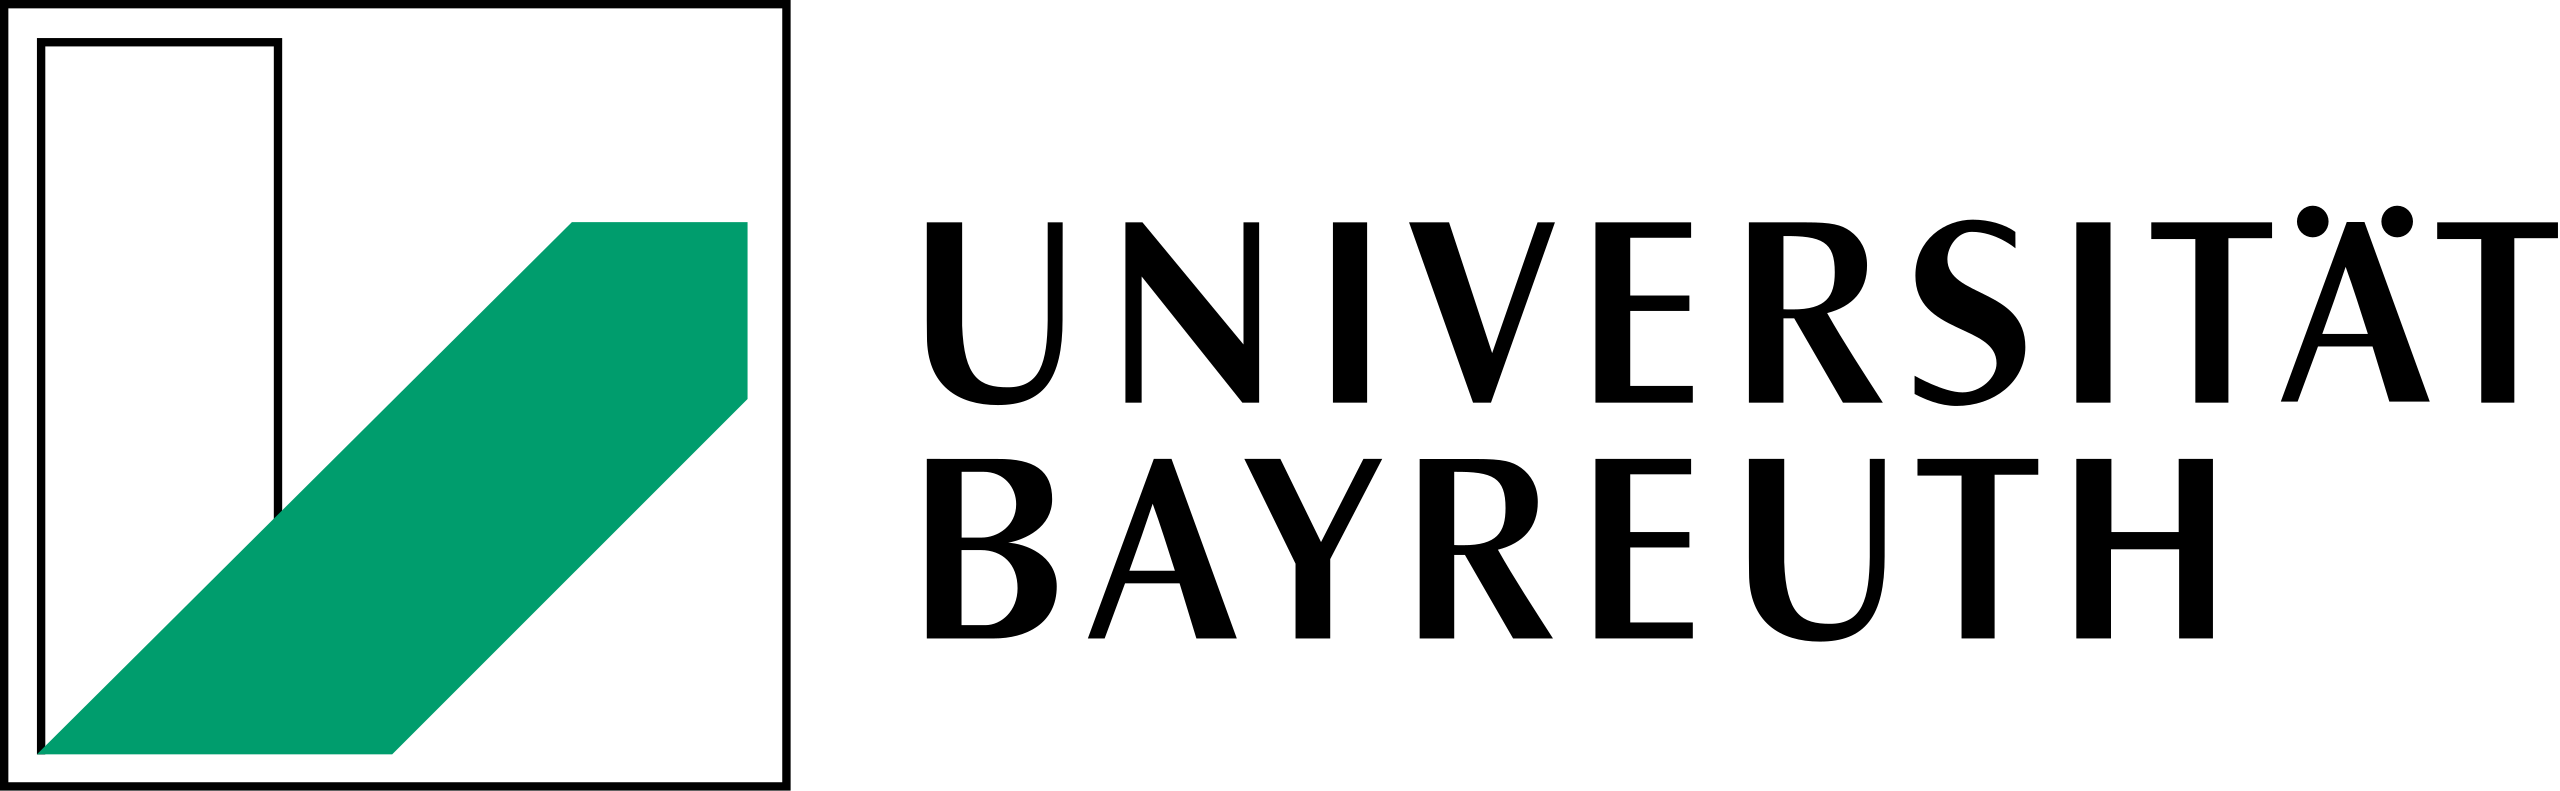
\includegraphics[height=2cm]{Uni_Logo_white_black.png}
}

\subject{\normalfont Master Thesis}
\title{Stabilizing Global Simulation in \gkw by the Introduction of the Parallel Electric Field \boldmath{$\Epar$}}
\author{Manuel Lippert}
\date{Submission date: \today}
\publishers{\textbf{Physics Department at the University of Bayreuth}\\
\vspace*{2em}
%\begin{tabular}{l l}
%First Supervisor: & Prof.\,Arthur\,G.\,Peeters\\
%Second Supervisor: & Dr.\,Florian\,Rath\\
%\end{tabular}
Supervisors:\\
Prof.\,Arthur\,G.\,Peeters\\
Dr.\,Florian\,Rath
}

\begin{document}
    \nonfrenchspacing

    \newgeometry{left=2.5cm,right=2.5cm}
    \maketitle
    \restoregeometry    

    \NewPage
\thispagestyle{empty}

\begin{center}
    \vspace*{3cm}
    \begin{tikzpicture}
        \clip(0,0)circle[x radius=3cm, y radius=4cm];
        \node{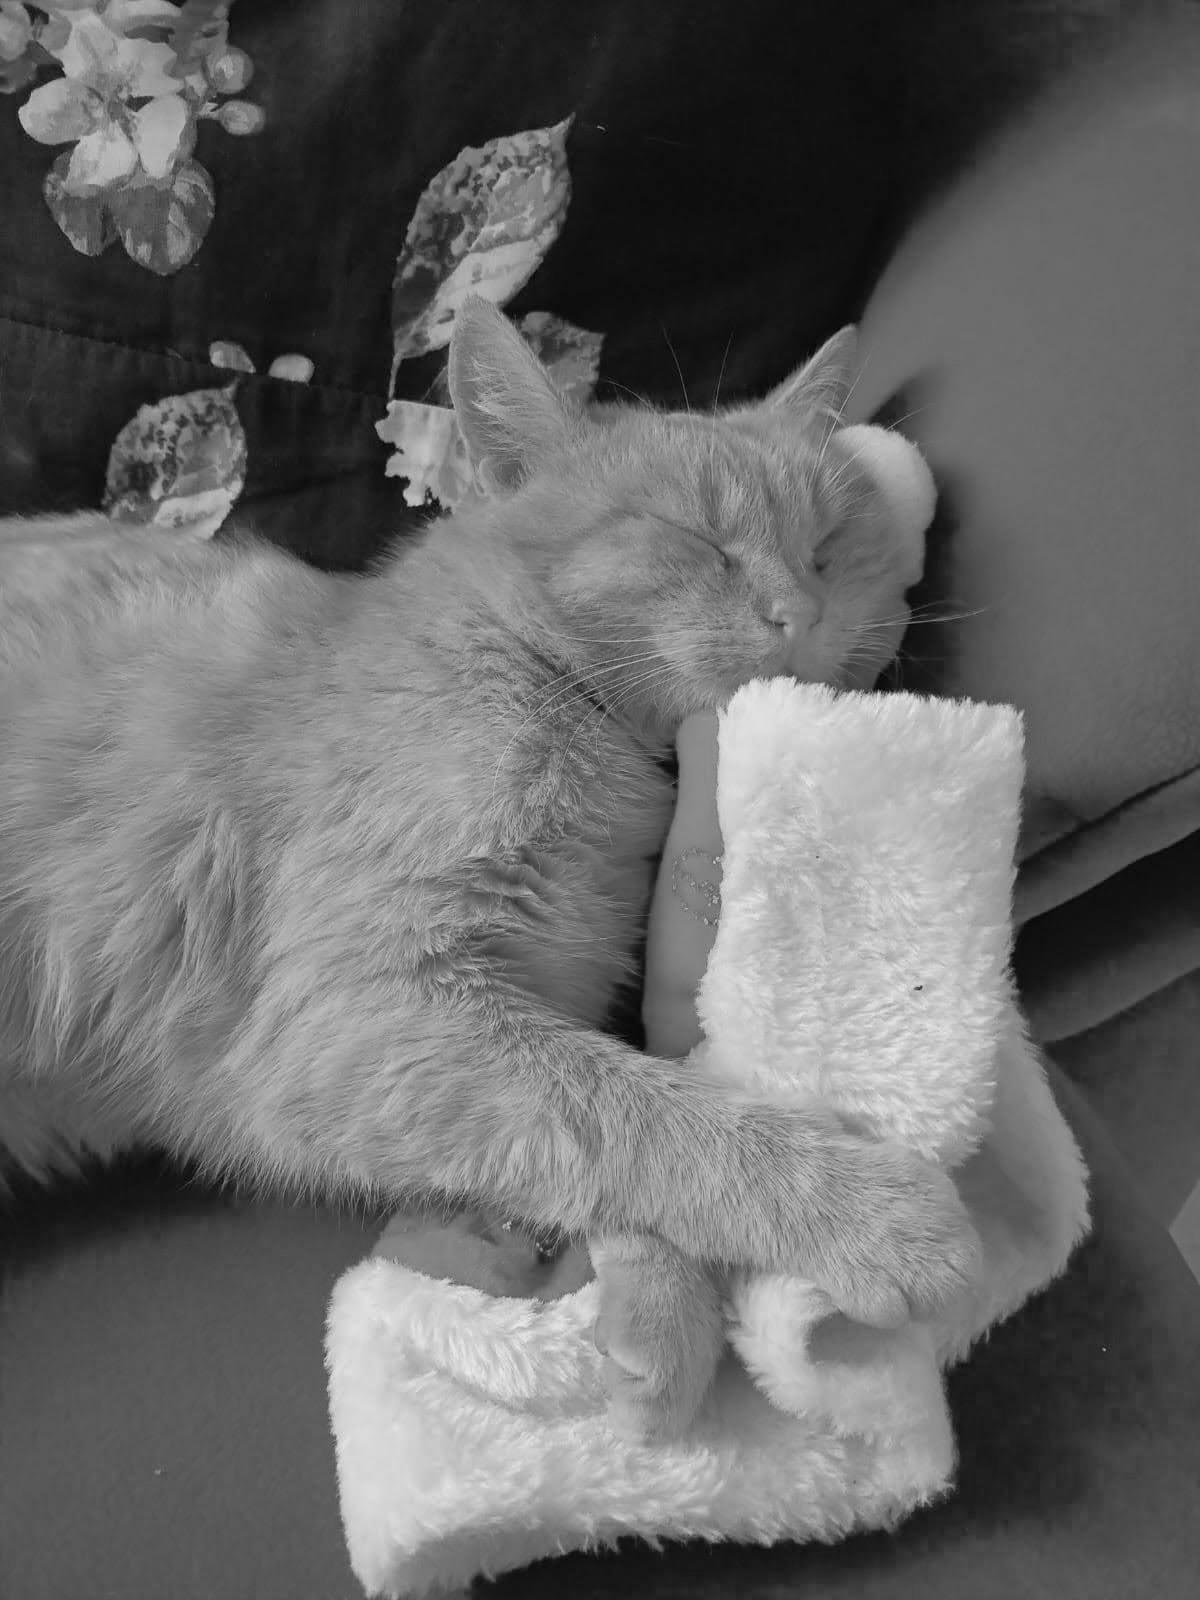
\includegraphics[width=6cm]{dedication/Leo1_Black-White.jpg}};
    \end{tikzpicture}
    \vspace{2cm}\\
    \gtrsymBorn~07.07.2020 - \gtrsymDied~09.08.2024 \\
    \bigskip
    This thesis is dedicated to my cat \textbf{Leo}\\ who is part of our family since July 2020.\\ He is the kindest cat I ever own.\\ During the pandemic we got very close together. \\ I will miss our walks together and your accompany in my life. \\ 
    \bigskip
    I love you.\\
    \bigskip
    Manuel Lippert\\
    % \today % Last edit August 10th
\end{center}
    \NewPage
\chapter*{Acknowledgement}
\label{chap:acknowledgement}

First, I would like to extend my greatest gratitude to my supervisor Prof. Arthur Peeters and Dr. Florian Rath. I would like to thank both of you for your guidance and support during the writing process of this thesis. \bigskip

I would like to thank René Meißner for the access to the festus cluster and Markus Hilt for the great technical support. \bigskip

Also, I would like to thank my best friend, Paul Schwanitz, for his support in many situations and the good discussions in- and outside of academia. In addition, I would like to thank Anna-Maria Pleyer and Fabian Eller for the great time of sharing the office together. \bigskip

I thank my sister Cornelia Lippert for proofreading this thesis, which shows me that I still have to improve my English spelling. \bigskip

Outside of academia, I would like to extend my gratitude to my parents, my brother, his wife and daughter, my sister and my girlfriend for their encouragement, endurance and support while writing this thesis. 
    %\NewPage
\chapter*{Abstract}
\label{chap:abstractENG}

Ion temperature gradient-driven turbulence (ITG) close to marginal stability exhibits zonal flow pattern formation on mesoscales, so-called $\exb$ staircase structures. Such pattern formation has been observed in local gradient-driven flux-tube simulations as well as global gradient-driven and global flux-driven studies. \bigskip

To reduce the computational effort for the simulations lower input parameter of {\gkw} (Gyro Kinetic Workshop) were tested to find the optimum of minimum resolution for the performed simulations. \bigskip

For convenience, a \texttt{python} script (\texttt{slurm\_monitor.py}) was written to monitor the simulation on the \texttt{btrzx1}-cluster and start/restart until the completion criterion is fulfilled. \bigskip

Furthermore, it is shown by multiple box size convergence scans that a mesoscale pattern  size of $\sim 57-76\,\rhoth$ is inherent to ITG-driven turbulence with Cyclone Base Case parameters in the local limit. This outcome also implies that a typical scale for avalanche-like transport is inherent to ITG-driven turbulence.

%\NewPage
\chapter*{Zusammenfassung}
\label{chap:abstractDE}

Ionen-Temperaturgradienten getriebene Turbulenzen (ITG) weisen nahe niedriger Stabilität Zonal Flow Strukturbildungen, sogenannte $\exb$ Treppenstrukturen, auf Mesoskalen auf. Solche Strukturbildungen wurden sowohl in lokal gradientengetriebene Flussschlauchsimulationen als auch in global gradientengetriebenen und global flussgetriebenen Untersuchungen entdeckt. \bigskip

Um den Aufwand der Berechnungen der Simulationen zu reduzieren wurden mehrere kleinere Inputparameter für {\gkw} (Gyro Kinetic Workshop) getestet um die optimal kleinste Auflösung für die ausgeführten Simulationen zu finden. \bigskip

Der Einfachheit halber wurde ein \texttt{python}-Skript (\texttt{slurm\_monitor.py}) geschrieben, was Simulationen auf den \texttt{btrzx1}-Cluster überwacht und gegebenenfalls startet/neustartet bis das Kriterium zur Vollendung erfüllt ist. \bigskip

Weiterhin wurde doch mehrere radiale konvergierende Boxgrößen-Scans gezeigt, dass eine Mesoskalengröße von $\sim 57-76\,\rhoth$ inhärent zur ITG getriebenen Turbulenz mit Cyclone Base Parameter in lokalen Limit ist. Dieses Ergebnis impliziert auch, dass eine typische Skala für den lawinenenartig Transport inhärent für die ITG getriebene Turbulenz ist.
    \NewPage
\chapter*{Declaration}
\label{chap:declaration}

The author states that every information, regarding this thesis can be found under the GitHub Repository with the link \url{https://github.com/ManeLippert/Masterthesis-Parallel-Electric-Field}.

    %
    %\thispagestyle{empty}
    %\NewPage
    \cleardoublepage
    \tableofcontents
    \cleardoublepage
    %
    % 1.Chapter Instruction
    % 1. Introduction

\NewPage
\chapter{Motivation}
\label{chap:motivation}

\thispagestyle{empty}
\newpage

% TODO: Write about cancellation problem

Plasma can be described in various theoretical models. The main two models are the Magnetohydrodynamics and the kinetic model. The key differences will be briefly explained in the following.
\begin{itemize}
    \item \textbf{Magnetohydrodynamics:}\\
        In Magnetohydrodynamics the plasma will be described as an electric conductiv fluid which carries current. Here, the electrons and ions are two mixed fluids expressed in the two-fluid theory. 
    \item \textbf{Kinetic Model:}\\
        In the kinetic model the plasma will be described in the sixdimensional phase space through the Vlasov equation. In combination with the Maxwell's equations is it possible to discribe the dynamics of the plasma as the Vlasov-Maxwell system. 
\end{itemize}
In both description macroscopic quantities will be used, i.e. density, velocity of the fluid and temperature. In this thesis the kinetic model will be covered in greater depth. The numerical diescription of such models can be seperate in the local and global description. Here, the global electromagnetic gyrokinetic simulations are suffering from numerical problems, mainly from the \textit{cancellation problem} \cite{Chen2001} examined in codes which uses the paticle-in-cell or the Eulerian methods \cite{Cummings_PHD}. This problem limits the electromagnetic investigations to extremely low plasma beta. \cite{Naitou1995} A high plasma beta value is always wanted since the fusion reaction rates ($\sim \beta^2$) and indic

The goal of this thesis is to lay the groundwork for the global electromagnetic gyrokinetic model for \gkw and to mitigate the cancellation problem in the local version of \gkw. For that purpose, the field equation for the induced electric field $\Epar$ gets implemented by using Faraday's law and the switch to \textit{f-version} in the local description of \gkw will be performed. The implementation of the field equation and its theory follows the Dissertation of Paul Charles Crandall\cite{Crandall_PHD}. Then, the new local electromagnetic model of \gkw will .

    % 2.Chapter Plasma Physics Basics
    % 2. Plasma Physics

\chapter{Plasma Physics Basics}
\label{chap:plasmaPhysics}

\thispagestyle{empty}
\newpage
    \section{Charged Particle Motion in Magnetic and Electric Field}
\label{sec:motion}

In magnetic confinement devices like the tokamak reactor, the charged particles experience forces caused by magnetic and electric fields which results in distinct motion under the associated force. Charged particles can be separated in species, e.g. electrons and ions, which will be later on not displayed in the governing equation. Throughout this thesis the charge $q$, the mass $m$ or the temperature $T$ indicate the quantities of a specific species, i.e., electrons or ions.

\subsection{Particle Motion perpendicular to the Magnetic Field}
\label{sub:gyromotion}

Due to the Lorentz force, particles with a velocity component perpendicular to the homogenous magnetic field $v_{\perp}$ undergo a circular motion in the plane perpendicular to the magnetic field [Fig. \ref{fig:perp-par-motion}(a)]. This type of motion has circular frequency, which is often referred to as \textit{cyclotron frequency} and is defined as
\begin{gather}
    \omega_\mathrm{c} = \frac{|q|B}{m}~,
    \label{eq:cyclotron}
\end{gather}
where $m$ and $q$ are the mass and the charge of the particle and $B$ the strength of the magnetic field. The radius, the so called \textit{Larmor radius}, of this motion is given by
\begin{gather}
    \rho = \frac{mv_{\perp}}{|q|B}
    \label{eq:Larmorradius}
\end{gather}
with the center often being referred to as \textit{gyrocenter}. Note that since the Lorentz force depends on the species charge of the particle, the circulation direction is the opposite between electron in ions.\\\bigskip

Due to Coulomb collisions the plasma gets thermalized. Together with the Maxwell-Boltzmann distribution the typical thermal velocity is
\begin{gather}
    \vth = \sqrt{\frac{2T}{m}}~,
    \label{eq:thermalVelocity}
\end{gather}
where $T$ represents the species temperature. Based on the thermal velocity $v_\mathrm{th}$ the \textit{thermal Larmor radius} gets introduced as \cite{Wesson2004}
\begin{gather}
    \rhoth = \frac{m\vth}{|q|B}~.
    \label{eq:thermalLarmorradius}
\end{gather}

\newpage

\subsection{Particle Motion parallel to the Magnetic Field}
\label{sub:parallelmotion}

In absence of forces in the direction parallel to the magnetic field the particles can move freely in parallel direction to the homogenous magnetic field. The velocity of this motion is of order of the thermal velocity $\vth$ and is dominated by electrons due to their lighter mass compared to ions ($v_\mathrm{th,e}/v_\mathrm{th,i} = 60$). 

When an electric field with a component parallel to the magnetic field $E_\parallel$ influences the plasma the charged particles are accelerated by the electric force
\begin{gather}
    F_{\parallel,E} = qE_\parallel~.
    \label{eq:forceElectricParallel}
\end{gather}
The parallel motion follows then from the equation of motion. Here the direction of the motion also depends on the species type [Fig. \ref{fig:perp-par-motion}(b)].\\\bigskip

Since magnetic fields are not always homogenous, an inhomogeneous magnetic field with its gradient $\nabla B$ containing a component parallel to the magnetic field which is given by
\begin{gather}
    \nabla_{\!\parallel} B = \frac{\vect{B}}{B} \cdot \nabla B 
    \label{eq:forceMagneticParallel}
\end{gather}
causes the force
\begin{gather}
    F_{\parallel,\nabla_{\!\parallel} B} = - \frac{mv^2_{\perp}}{2B} \nabla_{\!\parallel} B = - \mu \nabla_{\!\parallel} B~;~~~~\mu = \frac{mv^2_{\perp}}{2B}
    \label{eq:magneticMoment}
\end{gather}
with \textit{magnetic moment} $\mu$. The magnetic moment $\mu$ is an adabatic invariant (constant of motion) if the variation of the magnetic field over time is smaller than the inverse of the cyclotron frequency $\omega^{-1}_\mathrm{c}$ and the spatial variation is larger the Larmor radius $\rho_\mathrm{L}$. The resulting force has its application in the mirror effect where a charged particle gets reflected due to this force [Fig. \ref{fig:perp-par-motion}(c)]. \cite{Wesson2004}

\newpage

\begin{center}
    \captionsetup{type=figure}
    \begin{tabular}{c c c c c c}
        % \usetikzlibrary{mindmap,backgrounds}
% \usetikzlibrary{decorations.pathmorphing}
% \usetikzlibrary{decorations.markings}
% \usetikzlibrary{arrows.meta,bending}

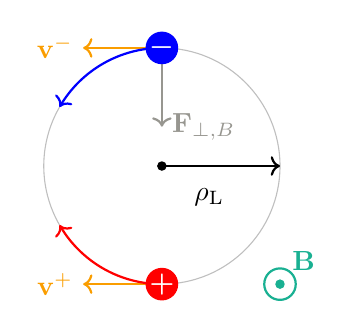
\begin{tikzpicture}
    % Circle
    \draw[lightgray] (0,0) circle (1.5);
    \filldraw (0,0) circle (1.5pt);
    % Force
    \draw[thick, Notagrey, <-] (90:0.5) node[right, Notagrey]{$\vect{F}_{\perp, B}$} -- ++ (90:1.0) node[coordinate] (x) {};
    % Larmor radius
    \draw[thick, black, ->] (0,0) -- ++(0:1.5);
    \draw (0.6,-0.4) node {$\rho_\mathrm{L}$};
    % Velocity
    \draw[thick,Notaorange, ->] (x) -- ++(180:1cm) node[left, Notaorange]{$\vect{v}^-$};
    \draw[thick,Notaorange, ->] (0,-1.5) -- ++(180:1cm) node[left, Notaorange]{$\vect{v}^+$};
    % Cyclontron freqency
    \draw[thick, ->, blue] (90:1.0*1.5) arc(90:150:1.0*1.5);
    \draw[thick, <-, red] (210:1.0*1.5) arc(210:270:1.0*1.5);
    % Charges
    \draw [fill=blue, blue] (x) circle (0.2) node[white, font=\boldmath]{$-$};
    \draw [fill=red, red] (0,-1.5) circle (0.2) node[white, font=\boldmath]{$+$};
    % Magnetic field
    \draw [thick, Notagreen] (1.5,-1.5) circle (0.2);
    \filldraw [Notagreen] (1.5,-1.5) circle (1.5pt);
    \draw (1.8,-1.2) node[Notagreen]{$\vect{B}$};
\end{tikzpicture} &
        % \usetikzlibrary{mindmap,backgrounds}
% \usetikzlibrary{decorations.pathmorphing}
% \usetikzlibrary{decorations.markings}
% \usetikzlibrary{arrows.meta,bending}

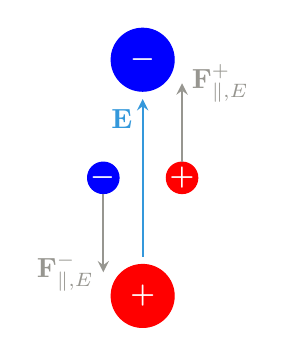
\begin{tikzpicture}
    % Charge
    \draw [fill=blue, blue] (0,1.5) circle (0.4) node[white, font=\boldmath]{$-$};
    \draw [fill=red, red] (0,-1.5) circle (0.4) node[white, font=\boldmath]{$+$};
    \draw [fill=blue, blue] (-0.5,0) circle (0.2) node[white, font=\boldmath]{$-$};
    \draw [fill=red, red] (0.5,0) circle (0.2) node[white, font=\boldmath]{$+$};
    % Electric field
    \draw[thick,Notablue, ->, >=stealth] (0,-1) -- (0,1) node[below left, Notablue] {$\vect{E}$};
    % Force
    \draw[thick, Notagrey, ->, >=stealth] (-0.5, -0.2) -- (-0.5, -1.2);
    \draw (-0.5, -1.2) node[left, Notagrey]{$\vect{F}^{-}_{\parallel,E}$};
    \draw[thick, Notagrey, ->, >=stealth] (0.5, 0.2) -- (0.5, 1.2);
    \draw (0.5, 1.2) node[right, Notagrey]{$\vect{F}^{+}_{\parallel,E}$};
\end{tikzpicture} &
        % \usetikzlibrary{mindmap,backgrounds}
% \usetikzlibrary{decorations.pathmorphing}
% \usetikzlibrary{decorations.markings}
% \usetikzlibrary{arrows.meta,bending}

{
\def\ang{36}
\def\Rx{0.7}
\def\Ry{1.14}
\def\h{0.5}
\def\H{3}
\def\W{4}
\def\NB{2}

\begin{tikzpicture}

	\coordinate (O) at (0,0);
	\coordinate (N) at (0,0.24*\H);
	\coordinate (M) at (0,0.45*\H);
	\coordinate (B) at (\ang:\H);

	% Magnetic momentum (1/2)
	\draw [thick, Notared] (0,\Ry) arc (90:270:{\Rx} and {\Ry});
	% Magnetic field
	\foreach \i [evaluate={\y=(0.34*\H)*\i^2/\NB; \out=1*\i^2; \in=180+10*\i^2; \f=0.80-0.10*\i;}] in {1,...,\NB}{
	  \draw [thick, Notagreen, <-, >=stealth] (-0.95*\H, 0.7*\y/\H) to[out= \out,in= \in,looseness=0.8] (0.25*\W, \y);
	  \draw [thick, Notagreen, <-, >=stealth] (-0.95*\H,-0.7*\y/\H) to[out=-\out,in=-\in,looseness=0.8] (0.25*\W,-\y);
	}
	\node [Notagreen] at (0.26*\W,0.52*\H) {$\vect{B}$};
	% Force
	\draw [thick, Notagrey, ->, >=stealth] ( 95:{\Rx} and {\Ry}) --++ (-25:0.8*\Ry) node[right=0, Notagrey] {$\vect{F}_{\parallel,\nabla_{\!\parallel} B}$};
	\draw [thick, Notagrey, ->, >=stealth] (-95:{\Rx} and {\Ry}) --++ ( 25:0.8*\Ry) node[right=1, Notagrey] {$\vect{F}_{\parallel,\nabla_{\!\parallel} B}$};
	% Magnetic momentum (2/2)
	\draw [thick, Notared] (0,\Ry) arc (90:-90:{\Rx} and {\Ry});
	\draw [thick, Notared, ->, >=stealth] (0,0) --++ (-0.3*\W,0) node[left, Notared] {$\vect{\mu}$};
	% Particle
	\filldraw [Notablue] (-95:{\Rx} and {\Ry}) circle (2pt);
	\filldraw [Notablue] ( 95:{\Rx} and {\Ry}) circle (2pt);
	\draw (-3,1) node[above right, Notablue]{Particle};

\end{tikzpicture}}\\[0.3cm]
        \textbf{(a)} & \textbf{(b)} & \textbf{(c)} \\
    \end{tabular}
    \captionof{figure}{Forces acting on a charged particle:\\
        \begin{tabular}{l l}
            \textbf{(a)} & Lorentz force $\vect{F}_{\perp, B}$ perpendicular to velocity $\vect{v}^\pm$ and \\
                         & magnetic field $\vect{B}$ which causes, circular motion with different \\
                         & directions for electron and ions, Lamor radius $\rho_\mathrm{L}$ and \\ 
                         & cyclotron frequency $\omega_\mathrm{c}$, \\
            \textbf{(b)} & Electric force $\vect{F}_{\parallel,E}^\pm$ with electric field $\vect{E}$,\\
            \textbf{(c)} & Mirror effect with force $\vect{F}_{\parallel,\nabla_{\!\parallel} B}$ and magnetic moment $\mu$ \\
                         & caused by an inhomogeneous magnetic field $\vect{B}$.  \\
        \end{tabular}
    }
    \label{fig:perp-par-motion}
\end{center}

\newpage

\subsection{Drifts in the Gyrocenter}
\label{sub:drift}

In the presence of a magnetic field (homogenous, inhomogeneous or perturbed) and electric fields the gyrocenter undergoes slow (compared to the thermal velocity $\vth$) drift motions perpendicular to the magnetic field. There are several examples for this drift motion. According to this thesis topic only the main three drift types will be covered in the following.

\begin{enumerate}
    \item {\boldmath $\exb$} \textbf{Drift:}\\
    If an electric field $\vect{E}$ with a perpendicular component together with the magnetic field $\vect{B}$ (both fields are homogenous) is present the acting Coulomb force and Lorentz force results into a drift of the gyrocenter with
    \begin{gather}
        \vect{v}_{E} = \frac{\vect{E}\times\vect{B}}{B^2}
        \label{eq:exb}
    \end{gather}
    which is called the $\exb$ drift. Since both acting forces direction depends on the species type the direction of the $\exb$ drift is for every species the same [Fig. \ref{fig:drift}(a)].
    \item {\boldmath $\nabla B$} \textbf{Drift:}\\
    Inhomogeneous magnetic field causes a gradient $\nabla B$ of the magnetic field. Because of that gradient the gyrocenter undergoes a $\nabla B$ drift defined by
    \begin{gather}
        \vect{v}_{\nabla B} = \frac{m v^2_{\perp}}{2 q}\frac{\vect{B}\times \nabla B}{B^3}~.
        \label{eq:gradB}
    \end{gather}
    The gradient of the magnetic field $\nabla B$ varies thereby on scales larger compared to the Larmor radius. The direction of the $\nabla B$ drift depends on the species type [Fig. \ref{fig:drift}(b)].
    \item \textbf{Curvature Drift:}\\
    Due to centrifugal force acting on the particle in a curved magnetic field the gyrocenter experiences a curvature drift according to
    \begin{gather}
        \vect{v}_{C} = \frac{m v^2_{\parallel}}{q}\frac{\vect{B}\times \vect{C}}{B^2} = \frac{m v^2_{\parallel}}{q} \frac{\vect{B}\times \nabla B}{B^3}~;\qquad\vect{C} = -(\vect{b}\cdot \nabla)\vect{b} = \frac{\nabla B}{B}~,
        \label{eq:curvature}
    \end{gather}
    where $\vect{b}$ is the unit vector along the magnetic field. To obtain the result for the curvature $\vect{C}$ in Eq. (\ref{eq:curvature}) the plasma pressure has to be small compared to the magnetic field strength $B$. In the form of Eq. (\ref{eq:curvature}) $\nabla B$ and curvature drift can be treated similarly. \cite{Wesson2004}
\end{enumerate}

% TODO: #4 Include more Drifts 

\newpage

\begin{center}
    \captionsetup{type=figure}
    \begin{tabular}{c c}
        % \usetikzlibrary{mindmap,backgrounds}
% \usetikzlibrary{decorations.pathmorphing}
% \usetikzlibrary{decorations.markings}
% \usetikzlibrary{arrows.meta,bending}

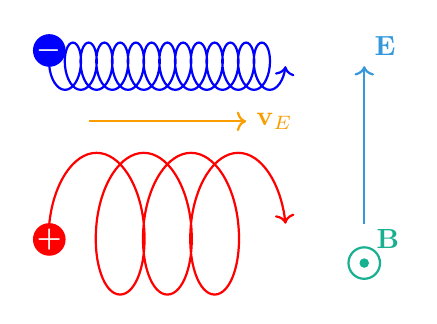
\begin{tikzpicture}
    % Electron
    \draw[thick,decoration={segment length=2mm, amplitude=0.3cm, coil},decorate,<-,blue] (3,0) -- (0,0);
    \draw [fill=blue, blue] (0,0.2) circle (0.2) node[white, font=\boldmath]{$-$};
    % Ion
    \draw[thick,decoration={coil, aspect = -0.5, amplitude = -0.9cm, segment length=6mm},decorate,<-,red] (3,-2) -- (0,-2);
    \draw [fill=red, red] (0,-2.2) circle (0.2) node[white, font=\boldmath]{$+$};
    % Electric field
    \draw[thick,Notablue, ->] (4,-2) -- (4,0) node[above right, Notablue]{$\vect{E}$};
    % Drift velocity
    \draw[thick,Notaorange, ->] (0.5,-0.7) -- (2.5,-0.7) node[right, Notaorange]{$\vect{v}_{E}$};
    % Magnetic field
    \draw [thick, Notagreen] (4,-2.5) circle (0.2);
    \filldraw [Notagreen] (4,-2.5) circle (1.5pt);
    \draw (4.3,-2.2) node[Notagreen]{$\vect{B}$};
\end{tikzpicture} &
        % \usetikzlibrary{mindmap,backgrounds}
% \usetikzlibrary{decorations.pathmorphing}
% \usetikzlibrary{decorations.markings}
% \usetikzlibrary{arrows.meta,bending}

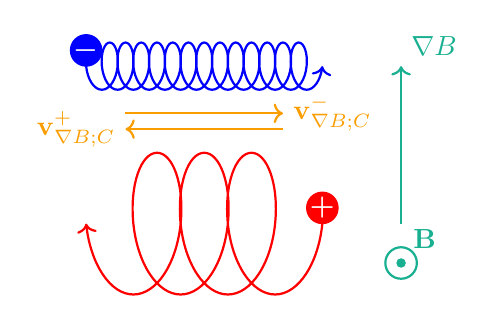
\begin{tikzpicture}
    % Electron
    \draw[thick,decoration={segment length=2mm, amplitude=0.3cm, coil},decorate,<-,blue] (3,0) -- (0,0);
    \draw [fill=blue, blue] (0,0.2) circle (0.2) node[white, font=\boldmath]{$-$};
    % Ion
    \draw[thick,decoration={coil, aspect = -0.5, amplitude = -0.9cm, segment length=6mm},decorate,<-,red] (0,-2) -- (3,-2);
    \draw [fill=red, red] (3,-1.8) circle (0.2) node[white, font=\boldmath]{$+$};
    % Grad B field
    \draw[thick,Notagreen, ->] (4,-2) -- (4,0) node[above right, Notagreen]{$\nabla B$};
    % Drift velocity
    \draw[thick,Notaorange, ->] (0.5,-0.6) -- (2.5,-0.6) node[right, Notaorange]{$\vect{v}^{-}_{\nabla B;C}$};
    \draw[thick,Notaorange, <-] (0.5,-0.8) node[left, Notaorange]{$\vect{v}^{+}_{\nabla B;C}$} -- (2.5,-0.8);
    % Magnetic field
    \draw [thick, Notagreen] (4,-2.5) circle (0.2);
    \filldraw [Notagreen] (4,-2.5) circle (1.5pt);
    \draw (4.3,-2.2) node[Notagreen]{$\vect{B}$};
\end{tikzpicture} \\[0.3cm]
        \textbf{(a)} & \textbf{(b)} \\
    \end{tabular}
    \captionof{figure}{Dirft motion in gyrocenter:\\
        \begin{tabular}{l l}
            \textbf{(a)} & $\exb$ Drift with drift velocity $\vect{v}_E$, electric field $\vect{E}$ and\\
                         & magnetic field $\vect{B}$,\\
            \textbf{(b)} & $\nabla B$ Drift/Curvature Drift with drift velocity $\vect{v}^{\pm}_{\nabla B;\kappa}$, magnetic\\
                         & field $\vect{B}$ and gradient of the magnetic field $\nabla B$. \\
        \end{tabular}
    }
    \label{fig:drift}
\end{center}

\newpage
    \newpage
\section{Magnetic Confinement and Plasma Rotation}
\label{sec:confinement}

In tokamak devices strong magnetic fields confine the hot plasma. As mentioned in Chapter \ref{sec:motion} a magnetic field forces a perpendicular particle motion and a motion which contains the gyro motion and slow perpendicular gyro center drifts. Because of the much smaller size of the Larmor radius compared to the device size $R$ the particle and energy losses are caused by the gyro center drift. To avoid additional loss of particles because of the parallel motion the field lines of the magnetic field in the tokamak devices is shaped like a torus. This type of geometry has nested surfaces with constant magnetic flux, so-called \textit{flux surfaces}, and magnetic field lines which lie on these surfaces. To maintain stability the magnetic field has a toroidal and a poloidal component. According to the force balance the magnetic field is equivalent to the plasma pressure which means on flux-surfaces the plasma pressure is constant. \cite{Stroth2018, Wesson2004} The toroidal component is produced by external coils whereas the poloidal component is provided by the toroidal plasma current. Together the components result in a magnetic field which follows helical trajectories [Fig \ref{fig:confinement}]. To characterize the quality of confinement the so-called \textit{plasma beta} is used and is given as
\begin{gather}
    \beta = \frac{nT}{B^2/2\mu_0}~,
\end{gather} 
with $n$ the plasma density, $T$ as temperature, $\mu_0$ the permeability in vacuum and the magnetic field strength $B$. Respectively, the plasma beta compares the thermal plasma pressure $nT$ to the ambient magnetic field pressure $B^2/2\mu_0 $. For fusion devices the plasma beta has to be a bit smaller than 1 ($\beta < 1$) for optimal confinement. In a tokamak reactor the plasma beta has a typical order of a few percent. \cite{Wesson2004}
\bigskip

The rotation of the plasma can be described in a co-rotating frame of reference, which is rigidly rotating with the velocity $\ueq$ and will be used later on in the derivation of the gyrokinetic equations in Chapter \ref{sec:lagrangian}. It assumend that the poloidal component of the plasma rotation is much smaller compared to the toridial component and will be neglected. With this assumption in mind the reference frame is chosen to move in the toridial direction exclusivly and its velocity $\ueq$ can be expressed as
\begin{gather}
    \ueq = \vect{\Omega} \times \x = R^2 \Omega \nabla \varphi~,
    \label{eq:rotvelocity}
\end{gather}
where $\vect{\Omega}$ is the constant angular frequency, $\varphi$ is the toroidal angle and $R \nabla\varphi$ is the unit vector in the toroidal direction. 

\newpage

Since the rotation of the plasma in the labortory frame is not a rigid body rotation, it will be characterized by the radial profile of the angular velocity $\hat{\Omega}(\psi)$. Then the angular frequency of the rotating frame $\Omega$ is chosen to match the plasma rotation on a certain point, i.e. $\Omega = \hat{\Omega}(\psi_r)$. The plasma rotation in the co-rotating frame of reference will be denoted as
\begin{gather}
    \omega_\varphi(\psi) = \hat{\Omega}(\psi) - \Omega.\
    \label{eq:refFramePlasmaFrequency}
\end{gather} 
with the rotation speed along the magnetic field line 
\begin{gather}
    u_\parallel = \frac{RB_\mathrm{t}}{B} \omega_\varphi (\psi)~,
    \label{eq:rotParallelVelocity}
\end{gather}
where $B_\mathrm{t}$ is the toridial component of the magnetic field. \cite{Peeters2009B}

\inputgraphicsHere{../pictures/theory/Tokamak-Torus.tex}{
	Toroidal flux surfaces in tokamak plasma with helical magnetic field (\textcolor{Notagreen}{green} line) in torus coordinates ($\psi$ (radial), $\varphi$ (toroidal), $\theta$ (poloidal)) or cylindrical coordinates ($z$, $R$, $-\varphi$). \cite{Barton2015}
}{fig:confinement}

\newpage

    % 3.Chapter Gyrokinetic Theory
    % 3. Derivation

\chapter{The Gyrokinetic Theory}
\label{chap:derivationGyrokineticEq}

\thispagestyle{empty}
\newpage

\bigskip
In this chapter the following scheme will be discussed:
\begin{enumerate}
    \item The Lagrangian $L$ for a particle in a electromagnetic field is reformulated in the fundamental one-form $\gamma$ according to 
        \begin{gather}
            \int \dt ~ L = \int \gamma~.
        \end{gather}
        From this point on the fundamental one-form and Lagrangian referes to the quantity $\gamma$. Then, the Lagrangian $\gamma$ will be transformed in the guiding center phase space and separated in its equilibrium and perturbated part. Through the Lie transformation the Lagrangian gets transformed into the gyrocenter phase space by eliminating the gyro phase. 
    \item Plugging the Lagrangian into the Euler-Lagrangian equation yields the equations of motions. From the equations of motion the Vlasov equation can be derived.
    \item The Vlasov equation solves for the density distribution function, which will be used to express the particle density $n$ and current $\vecj$ with the moments of the distribution function. 
    \item Particle density $n$ and current $\vecj$ will then be plugged into the Maxwell's equations, i.e. the field equations.
    \item The cancellation problem will be discussed and the mitigation technique will be introduced for {\gkw}.
\end{enumerate}

This chapter is based on the Dissertation of Tilman Dannert\cite{Dannert_PHD} and the derivation document provided by the {\gkw} group\cite{GKWDerivation}. The derivation of Faraday's law in Chapter \ref{sub:fieldEpar} is based on the disseration of Paul Crandall\cite{Crandall_PHD}.

\newpage
    \section{Gyrokinetic Ordering}
\label{sec:gyroordering}

% The typical spatio-temporal scales connected to the dynamics in a tokamak plasma allow for the so-called \textit{gyrokinetic ordering} as outlined below. The fast gyromotion is much smaller compared to typical  time scales connected to turbulence ($\omega/\omega_\mathrm{c} \sim 10^{-3})$. The length scales of the turbulence are associated with the wave vector $\vect{k}$ which can be seperated into a perpendicular component $k_\perp = |\vect{k} \times \vect{b}|$ and a parallel component $k_\parallel = |\vect{k} \cdot \vect{b}|$ where $\vect{b}$ is parallel to the poloidal component of the magnetic field. The perpendicular component $k_\perp$ is of the order of the thermal Larmor radius $k_\perp^{-1} \sim \rhoth$ which is significantly smaller than the scale on which the equilibrium density $n_0$ varies, which can be expressed with the gradient length $L_\mathrm{n} = |\nabla \ln n_0 |^{-1}$. The gradient length compares with the machine size $R$ which leads to the normalized thermal Larmor radius $\rho_* = \rhoth/R \sim 10^{-3} - 10^{-4}$ with $R$ as major radius of the tokamak. The parallel component $k_\parallel$ on the other hand scales with the machine size $R$. Experiments show that in the core plasma the fluctuation amplitude of the density perturbation $\delta n/n_0$ and magnetic field fluctuation $\delta B/B_0$, with $B_0$ as strength of the magnetic field in equilibrium, is of order $\sim 10^{-4}$. Together this separation result in the following
% \begin{gather}
% 	\frac{\omega}{\omega_\mathrm{c}} \sim \frac{k_\parallel}{k_\perp} \sim \frac{\rhoth}{L_\mathrm{n}} \sim \frac{\delta n}{n_0} \sim \frac{\delta B}{B_0} \sim \frac{v_\mathrm{d}}{\vth} \sim \epsilon_\mathrm{g}
% 	\label{eq:gyroordering}
% \end{gather}
% with $\epsilon_\mathrm{g} \ll 1$ which applies to the typical dynamics of a fusion core plasma. \cite{Brizard2007,Garbet2010} The gyrokinetic ordering allows formulating reduced governing equations referred to as the gyrokinetic formalism.

% \newpage 

In the derivation of the gyrokinetic theory the aim is to decouple the effect of small-scale, small amplitude fluctuations of the plasma in the Langrangian. For this it is chosen to take the properties of fluctuations as small parameter, which will get in the ordering assumptions applied in gyrokinetic theory \cite{Brizard2007}
\begin{gather}
	\begin{aligned}
		\frac{\abs{\vect{A_1}}}{\abs{\vect{A_0}}} &\sim \frac{\Phi_1}{\Phi_0} \sim \epsilon_\delta \ll 1 \\[0.3cm]
		\rho \frac{\nabla B_0}{B_0} &\sim \rho \frac{\nabla E_0}{E_0} \sim \frac{\rho}{L_B} \sim \epsilon_B \ll 1 \\[0.3cm]
		k_\perp \rho &\sim \epsilon_\perp \sim 1 \\[0.3cm]
		\frac{\omega}{\omega_\mathrm{c}} &\sim \epsilon_\omega \ll 1
	\end{aligned}
	\label{eq:gyroordering}
\end{gather}
where $\vect{A}$ and $\Phi$ are the vector and scalar potentials, $\vect{B}$ and $\vect{E}$ are the magnetic and electric fields, $\omega$ and $k_\perp$ are the typical mode frequency and perpendicular wavenumber defined as $k_\perp = |\vect{k} \times \vect{b}|$, $\rho$ and $\omega_\mathrm{c}$ are the Larmor radius and cyclotron frequency and $L_B$ the equilibrium magnetic length scale. The equilibrium quantities are denoted with 0 and the fluctuations with 1 subscript. \bigskip

The above-mentioned equations state that fluctuations have a much smaller magnitude than the corresponding equilibrium values, their typical timescale is much slower than the Larmor frequency, their characteristic length scale is of the order of the Larmor radius, and it is typically much shorter the equilibrium spatial variation scale. Teh gyrokinetic equations are valid under these ordering assumptions. \bigskip

The small parameters $\epsilon_\delta$, $\epsilon_B$, $\epsilon_\perp$ and $\epsilon_\omega$ are due to different physical but in practice it is assumed that they are of simular order and substitute them with one parameter. For the derivation of the gyrokinetic equations of GKW all derived equations are evaluated up to the first order of the ratio of the reference thermal Larmor radius $\rhothref$ and the equilibrium magnetic length scale $L_B$ as small parameter and is defined as \cite{Derivation}
\begin{gather}
	\rhost = \frac{\rhothref}{L_B} = \frac{\mref \vthref}{e \Bref} \sim \epsilon_B \sim \epsilon_\delta \sim \epsilon_\omega~.
	\label{eq:rhostar}
\end{gather}

% TODO: #5 Rewrite Ordering with seperate section and include formulas for length scales
    \newpage
\section{Gyrokinetic Lagrangian (Fundamental One-Form)}
\label{sec:lagrangian}

\subsection{Lagrangian in Patricle Phase Space}
\label{sub:particleLagrangian}

The Lagrangian of a particle $\gamma$ with mass $m$ and charge number $Z$ in the electro magnetic field will be described through the particle position $\x$ and the velocity $\velo$ as coordinates $\{\x, \velo \}$ and can be written as
\begin{gather}
    \gamma = \gamma_\nu \dz^\nu = \underbrace{\left(m\vect{v} + Ze\vect{A}(\vect{x}) \right)}_{\mathrm{Sympletic~Part}}\cdot\;\dx - \underbrace{\left(\frac{1}{2}mv^2 + Ze\Phi(\x)\right)}_{\mathrm{Hamiltonian}~H(\x,\velo)} \dt ~,
    \label{eq:particleLagrangian}
\end{gather}
where $\A$ and $\Phi$ are the vector and scalar potential, $\nu$ indexes the six coordinates, and Einstein notation is applied. This form is also known as fundamental one-form. \bigskip

The defined Lagrangian $\gamma$ will then be transformed in the rotating frame of reference [Ch. \ref{sec:confinement}], which can be achieved the following Lorentz transformation
\begin{gather}
    \velo \rightarrow \velo + \ueq \qquad \vect{E} \rightarrow \vect{E} + \ueq \times \vect{B} \qquad \Phi \rightarrow \Phi + \A \cdot \ueq ~.
\end{gather}
After performing the transformation outlined in Ref. \citenum{Peeters2009B} the Lagrangian $\gamma$ becomes
\begin{gather}
    \gamma = \left(m\vect{v} + m\ueq + Ze\vect{A}(\vect{x}) \right) \cdot \dx - \left(\frac{1}{2}mv^2 - \frac{1}{2}mu_0^2 + Ze\Phi(\x)\right) \dt ~.
    \label{eq:particleLagrangian}
\end{gather} 

In the next step small scale perturbations of the electromagnetic field gets introduced as following
\begin{gather}
    \Phi = \Phi_0 + \Phi_1 \qquad \A = \A_0 + \A_1~.
    \label{eq:electromagneticPertubation}
\end{gather}
Here, it is assumend that the equilibrium electric field is zero in a stationary plasma, but it will be kept in case for finite plasma rotation. According to the gyrokinetic ordering [Ch. \ref{sec:gyroordering}] the perturbations are in the first order of $\rhost$. Taking everything into account the Lagrangian in the particle phase space with perturbations can be written as
\begin{gather}
    \begin{aligned}
        \gamma   &= \gamma_0 + \gamma_1 \\
        \gamma_0 &= \left(m\vect{v} + m\ueq + Ze\vect{A}_0(\vect{x}) \right) \cdot \dx - \left(\frac{1}{2}mv^2 - \frac{1}{2}mu_0^2 + Ze\Phi_0(\x)\right) \dt \\
        \gamma_1 &= Ze\vect{A}_1(\x) \cdot \dx - Ze \Phi_1(\x)\;\dt~.
    \end{aligned}
    \label{eq:particlePertubationLagrangian}
\end{gather}

\subsection{Lagrangian in Guiding Center Phase Space}
\label{sub:guidingcenterLagrangian}

For the description of charged particle behaviour in the tokamak device the \textit{guiding center coordinates} are used [Fig. \ref{fig:guidingcenterCoords}]. This set of coordinates are defined as the following
\begin{gather}
    \begin{aligned}
        \X(\x,\velo) &= \x - \rrho &\qquad v_\parallel &= \velo \cdot \vect{b}(\x) \\
        \mu(\x,\velo) &= \frac{m v_\perp^2(\x)}{2B(\x)} &\qquad \theta(\x,\velo) &= \arccos\left(\frac{1}{v_\perp}\left(\vect{b}(\x) \times \velo\right)\cdot \hat{\vect{e}}_1\right)~,\\
    \end{aligned}
    \label{eq:guidingcenterCoords}
\end{gather}
where the guiding center follows the magnetic field with the parallel velocity $v_{\parallel}$. The gyromotion is described together with the magnetic moment $\mu$, the guiding center $\vect{X}$ and the gyro phase $\theta$ which gives a parameter set of six quantities $\{\vect{X}, v_{\parallel}, \mu, \theta\}$. Vector $\vect{b}(\x)$ is the unit vector in the direction of the equilibrium magnetic field and $\vect{r} = \rho(\x,\velo)\vect{a}(\x,\velo)$ is the vector pointing from the guiding center to the particles postion, which is defined by the unit vector $\vect{a}(\x,\velo)$ and its length is the Lamor radius $\rho(\x,\velo)$. The unit vector $\vect{a}(\x,\velo)$ can be expressed in a local orthonormal basis as the function of the gyroangle $\theta$ 
\begin{gather}
    \vect{a}(\theta) = \hat{\vect{e}}_1 \cos\theta + \hat{\vect{e}}_2 \sin\theta~.
    \label{eq:guidingcenterUnitvect}
\end{gather} 
The vectors $\vect{b}$, $\hat{\vect{e}}_1$ and $\hat{\vect{e}}_2$ form a local Cartesian coordinate system at the guiding center position. 

\inputgraphicsHere{../pictures/Theory/Guiding-Center-Coordinates.tex}{
    Sketch of guiding center coordinates where the charged particle performs a circular motion around the guiding center. \cite{Krommes2000}
}{fig:guidingcenterCoords}

\newpage

To transform the fundamental one-from into the guiding center coordinates the following relation will be used
\begin{gather}
    \Gamma_\eta = \gamma_\nu \frac{\dz^\nu}{\dZ^\eta}~,
    \label{eq:trafoLagrangian}
\end{gather} 
where $\Gamma_\eta$ is a component of the guiding center fundamental one-form. To calculate the new coordinates the transformation [Eq. (\ref{eq:guidingcenterCoords})] have to be inverted to provide the old coordinates as function of the new one $z(Z)$. Here, the direct transformation is clearly uniquely determined if the magnetic field is known at the particle postion. However, the inverse transformation is not uniquely due to the dependence of the Larmor radius $\rho$ on magnetic field at the particle position $\x$. Taylor expansion of the Larmor radius $\rho$ around the guiding center $\X$ yields $\rho(\x) \approx \rho(\X)$. Note, that terms of order $\rho^2$, which leads to second order terms in $\rhost$, will get neglected due to the gyrokinetic ordering. The Larmor radius $\rho$ also depends on the velocity $\velo$ in particle phase space [Eq. (\ref{eq:Larmorradius})], or the magnetic moment $\mu$ in the guiding center phase space through the formular
\begin{gather}
    \rho(\X, \mu) = \frac{1}{Ze} \sqrt{\frac{2\mu m}{B(\X)}}~.
    \label{eq:guidingcenterLarmorradius}
\end{gather}
This dependence will be only used if greater clarity is needed. With result of the taylor expansion the particle position $\x$ can be expressed with the guiding center coordinates as 
\begin{gather}
    \x(\X,\theta) \approx \X + \rho(\X)\vect{a}(\theta)~.
    \label{eq:guidingcenterParticleCoord}
\end{gather}
The particle velocity $\velo$ is the sum of the velocity along the magnetic field $v_\parallel$, the gyration velocity $\velo_\perp$ and the drift velocity, which will be neglected because the particle drifts can be described by the motion of the guiding center. So to summarize the velocity $\velo$ in the guiding center frame can be expressed as 
\begin{gather}
    \velo = v_\parallel \vect{b}(\x) + \velo_\perp = v_\parallel \vect{b}(\x) + \rho(\x) \dot{\vect{a}}(\theta)~.
    \label{eq:guidingcenterVelocity}
\end{gather}
Applying Taylor expansion again around the guding center $\X$ teh following expression can be obtained
\begin{gather}
    \velo(\X, v_\parallel, \mu, \theta) \approx v_\parallel \left[\vect{b}(\X) + \partial_{\X} \vect{b}(\X) \cdot \vect{a}(\theta)\rho(\X,\mu) \right] + \rho(\X,\mu)\dot{\vect{a}}(\theta)~.
    \label{eq:guidingcenterVelocityCoord}
\end{gather}

Now, the transformation [Eq. (\ref{eq:trafoLagrangian})] can be applied to express the fundamental one-form in the new coordinates with the following components
\begin{gather}
    \begin{aligned}
        \Gamma_{X^i} &= \gamma_{x^j} \frac{\mathrm{d}x^j}{\mathrm{d}X^i} + \gamma_{v^j} \frac{\mathrm{d}v^j}{\mathrm{d}X^i} + \gamma_{t} \frac{\mathrm{d}t}{\mathrm{d}X^i} = \gamma_{x^j} \frac{\mathrm{d}x^j}{\mathrm{d}X^i} &\qquad \Gamma_{v_\parallel} &= \gamma_{x^j} \frac{\mathrm{d}x^j}{\mathrm{d}v_\parallel} + \gamma_{v^j} \frac{\mathrm{d}v^j}{\mathrm{d}v_\parallel} = 0 \\
        \Gamma_{\mu} &= \gamma_{x^j} \frac{\mathrm{d}x^j}{\mathrm{d}\mu}                                                                                                                                                      &\qquad \Gamma_{\theta}      &= \gamma_{x^j} \frac{\mathrm{d}x^j}{\mathrm{d}\theta}\\
        \Gamma_{t}   &= \gamma_{t} \frac{\mathrm{d}t}{\mathrm{d}t} + \mu B(\X) = \gamma_t + \mu B(\X) ~. & & \\
    \end{aligned}
    \label{eq:guidingcenterLagrangianTrafo}
\end{gather}
Note, that to the Hamiltonian part $\Gamma_t$ the energy term of the magnetic field $B$ at the guiding center $\X$ has to be added, due to the circular motion of the particle around the center.
\newpage
In Equation (\ref{eq:guidingcenterLagrangianTrafo}) the components of the fundamental one-form of the particle phase space $\gamma_\nu$ and the equation for $\velo$ in guiding center coordinates [Eq. (\ref{eq:guidingcenterVelocityCoord})] will be inserted and the Taylor expansion up to the first order applied for terms containing the particle position $\x$ as argument. After that the gyroaveraging operator will be used, which is defined as the integral over the gyrophase $\theta$
\begin{gather}
    \langle \;\cdot\; \rangle = \frac{1}{2\pi} \int_{0}^{2\pi} \dtheta ~ (\;\cdot\;)~.
    \label{eq:gyroaveraging}
\end{gather}
Due to the definition of the vector $\vect{a}$ [Eq. (\ref{eq:guidingcenterUnitvect})] the first order terms in $\vect{a}$ and $\dot{\vect{a}}$ disappear under gyroaveraging. Following all the previous steps, one can obtain
\begin{gather}
    \begin{aligned}
        \langle \Gamma_{\X} \rangle &= m v_\parallel b_i(\X) + mu_{0i} + Ze\A(\X) &\qquad \langle \Gamma_{v_\parallel} \rangle &= 0 \\
        \langle \Gamma_{\mu} \rangle &= 0                                           &\qquad \langle \Gamma_{\theta}      \rangle &= \frac{2\mu m}{Ze}\\
        \langle \Gamma_{t}   \rangle &= - \left(\frac{1}{2}mv_\parallel^2 - \frac{1}{2}mu_0^2 + Ze\Phi(\X) + \mu B(\X) \right) ~, & & \\
    \end{aligned}
    \label{eq:guidingcenterLagrangianTrafoAverage}
\end{gather}
which results in the fundamental one-form in guiding center coordinates
\begin{gather}
    \begin{aligned}
        \langle \Gamma \rangle =  &\left(m v_\parallel \vect{b}(\X) + m\ueq + Ze\A(\X)\right) \cdot \mathrm{d}\X + \frac{2\mu m}{Ze} \mathrm{d}\theta \\
                                  &- \left(\frac{1}{2}mv_\parallel^2 - \frac{1}{2}mu_0^2 + Ze\Phi(\X) + \mu B(\X) \right) \mathrm{d}t~.
    \end{aligned}
    \label{eq:guidingcenterLagrangian}
\end{gather}
Note that as a consequence of the Lagrangian being independent of the gyrophase $\theta$, the magnetic moment $\mu$ (the associated conjugated coordinate pair of $\theta$) becomes an invariant of the motion ($\dot{\mu} = 0$). \bigskip

As in Chapter \ref{sub:particleLagrangian} perturbations [Eq. (\ref{eq:electromagneticPertubation})] will get introduced to the guiding center Lagrangian. The transformation of the equilibrium part is already performed above, so only the pertrubation part with the pertubated Lagrangian in the particle phase space $\gamma_1$ has to be transfromed to the guiding center phase space. The transformation is analogous to the calculation before, the key difference is that the fluctuations quantities vary on a small length scale and Taylor expansion around the guiding center $\X$ can not be applied advantageous. Their values have to be taken at the particle position, which is a function of the gyroangle in guiding center coordinates. After this clearification the components of the perturbated Lagrangian in the guiding center phase space can be written as
\begin{gather}
    \begin{aligned}
        \Gamma_{1, X^i} &= \gamma_{1, x^j} \frac{\mathrm{d}x^j}{\mathrm{d}X^i} &\qquad \Gamma_{1. v_\parallel} &= 0\\
        \Gamma_{1, \mu} &= \gamma_{1, x^j} \frac{\mathrm{d}x^j}{\mathrm{d}\mu} &\qquad \Gamma_{1, \theta}      &= \gamma_{1, x^j} \frac{\mathrm{d}x^j}{\mathrm{d}\theta}\\
        \Gamma_{1, t}   &= \gamma_{1,t} ~. & & \\
    \end{aligned}
    \label{eq:guidingcenterPertrubationLagrangianTrafo}
\end{gather}
After inserting the components of the perturbated Lagrangian $\gamma_1$ and neglecting terms of order $\rho^2$, due to gyrokinetic ordering, the pertrubated compentents in the guiding center coordinates can be expressed as
\begin{gather}
    \begin{aligned}
        \Gamma_{1, \X} &\approx Ze\A_{1}(\x)                                                           &\qquad \Gamma_{1. v_\parallel} &= 0 \\
        \Gamma_{1, \mu} &= \frac{Z}{\abs{Z}} \frac{1}{v_\perp(\X,\mu)} \A_1(\x) \cdot \vect{a}(\theta) &\qquad \Gamma_{1, \theta}      &= \frac{Z}{\abs{Z}} \frac{2\mu}{v_\perp(\X,\mu)} \A_1(\x) \cdot \frac{\mathrm{d}\vect{a}(\theta)}{\mathrm{d}\theta} \\
        \Gamma_{1, t}   &= -Ze \Phi_1(\x) ~. & & \\
    \end{aligned}
    \label{eq:guidingcenterPertrubationLagrangian}
\end{gather}
Finally, the fundamental one-form in the guiding center phase space $\Gamma$ with perturbation can be written as
\begin{gather}
    \begin{aligned}
        \Gamma                   &= \langle \Gamma_0 \rangle + \Gamma_1 \\
        \langle \Gamma_0 \rangle &= \left(m v_\parallel \vect{b}(\X) + m\ueq + Ze\A_0(\X)\right) \cdot \mathrm{d}\X + \frac{2\mu m}{Ze} \mathrm{d}\theta \\
                                 &\quad - \left(\frac{1}{2}mv_\parallel^2 - \frac{1}{2}mu_0^2 + Ze\Phi_0(\X) + \mu B_0(\X) \right) \mathrm{d}t \\
        \Gamma_1                 &= Ze\A_{1}(\x) \cdot \mathrm{d}\X + \frac{Z}{\abs{Z}} \frac{1}{v_\perp} \A_1(\x) \cdot \vect{a} \mathrm{d}\mu + \frac{Z}{\abs{Z}} \frac{2\mu}{v_\perp} \A_1(\x) \cdot \frac{\mathrm{d}\vect{a}}{\mathrm{d}\theta} \mathrm{d}\theta - Ze \Phi_1(\x) \mathrm{d}t~. 
    \end{aligned}
\end{gather}

\newpage

\subsection{Lagrangian in Gyrocenter Phase Space}
\label{sub:gyrocenterLagrangian}

The transformation of the guiding center Lagrangian $\Gamma$ into the Lagrangian in gyrocenter phase space $\bar{\Gamma}$ aims to remove the gyroangle $\theta$ dependence resulting from the introduction of fluctuations. To destinguish between the guiding center and the gyrocenter coordinates all quantities associated with the gyrocenter are getting an overbar, i.e. $\bar{\Gamma}$.  The new set of gyrocenter coordinates are given by $\{\bar{\X}, \bar{v}_\parallel, \bar{\mu}\}$, but these coordinates will not been used in this thesis. Since the derivation of fundamental the one-form in gyrocenter phase space $\bar{\Gamma}$ uses the Lie transform pertubation method, which is beyond the scopes of this thesis, the reader is referred to the Refs. \citenum{Dannert_PHD} and \citenum{Derivation} for more details. The Lagrangian in the gyrocenter phase space can be expressed as
\begin{gather}
    \begin{aligned}
        \bar{\Gamma} &= \bar{\Gamma}_0 + \bar{\Gamma}_1 \\
                     &= \left(mv_\parallel \vect{b}_0(\X) + m\ueq + Ze\left(\A_0(\X) + \bar{\A}_1(\X)\right)\right) \cdot \mathrm{d}\X + \frac{2\mu m}{Ze} \mathrm{d}\theta \\
                     &\quad - \left(\frac{1}{2} m \left(v_\parallel^2 - u_0^2 \right) + Ze \left(\Phi_0(\X) + \bar{\Phi}_1(\X)\right) + \mu\left(B_0(\X) + \bar{B}_{1\parallel}(\X)\right)\right)\;\dt~,
    \end{aligned}
    \label{eq:gyrocenterPertrubationLagrangian}
\end{gather}
where $B_0$ is the equilibrium magnetic field and $\bar{B}_{1\parallel}$ is the magnetic field introduced by the vector potential $\A_1$. Note, that the pertubations of the scalar and vector potential will be seperated into an oscillating and a gyroaveraged part which will be expressed as
\begin{gather}
    \Phi_1 = \widetilde{\Phi}_1 + \langle \Phi_1 \rangle  \qquad \A_1 = \widetilde{\A}_1 + \langle \A_1 \rangle~,
    \label{eq:electromagneticPertubationSeperated}
\end{gather}
although the oscillating parts will be added to the gauge function of the Lie transformation and will not be included in the Lagrangian of the gyrocenter. The quantities $\bar{\Phi}_1$, $\bar{\A}_1$ and $\bar{B}_{1\parallel}$ are the shorter notation of following gyroaveraged quantities defined as
\begin{gather}
    \begin{aligned}
        \langle \Phi_1(\x) \rangle &= J_0(\lambda) \Phi_1(\X) = \bar{\Phi}_1(\X) \\
        \langle \A_1(\x)   \rangle &= J_0(\lambda) \A_1(\X) = \bar{\A}_1(\X) \\ 
        Ze \langle \A_1(\x) \cdot \velo_\perp (\X,\mu,\theta) \rangle &= - \hat{J}_1(\lambda) \mu B_{1 \parallel}(\X) = \mu\bar{B}_{1\parallel}(\X)~,
    \end{aligned}
    \label{eq:gyrocenterGyroaveragedQuantitiesFourierspace}
\end{gather}
with $J_0$ as the zeroth order Bessel function and $I_1$ as the modified first order Bessel function of first kind defined as $I_1(\lambda) = 2/\lambda \, J_1(\lambda)$.
The components of the gyrocenter Lagrangian are again indepedent of the gyrophase $\theta$, and therefore the teh magnetic moment $\mu$ remains in the gyrocenter pahse space an invariant of motion.

\newpage
\subsection{Bessel Function}
\label{sub:Besselfunction}

To obtain Equation (\ref{eq:gyrocenterGyroaveragedQuantitiesFourierspace}) the process of gyroaveraging will be performend in the Fourier space as follows
\begin{gather}
    \begin{aligned}
        \langle \vect{G}(\x) \rangle &= \langle \vect{G}(\X + \vect{r}) \rangle = \langle \int \mathrm{d}\vect{k} ~ \hat{\vect{G}}(\vect{k}) e^{i \vect{k} \cdot (\X + \vect{r})} \rangle \\
                                     &= \frac{1}{2\pi} \int_{0}^{2\pi} \dtheta ~ \int \mathrm{d}\vect{k} ~ \hat{\vect{G}}(\vect{k}) e^{i \vect{k} \cdot \X} e^{ i k_\perp \rho \cos \theta} \\
                                     &= \int \mathrm{d}\vect{k} ~ \hat{\vect{G}}(\vect{k}) e^{i \vect{k} \cdot \X} \underbrace{\frac{1}{2\pi} \int_{0}^{2\pi} \dtheta ~ e^{ i k_\perp \rho \cos \theta}}_{J_0(\rho k_\perp)}\\
                                     &= \int \mathrm{d}\vect{k} ~ J_0(\rho k_\perp) \hat{\vect{G}}(\vect{k}) e^{i \vect{k} \cdot \X} = J_0(\lambda) \vect{G}(\X)~,
    \end{aligned}
    \label{eq:gyroOperator}
\end{gather}
where the wave vector $\vect{k}$ is defined as $\vect{k} = \hat{e}_1 k_\perp$. The argument $\lambda$ is given by $i \rho \nabla_{\!\perp}$ which is the inverse Fourier transformated expression of $\rho k_\perp$. The Bessel function $J_0$ is sometimes also referred to as gyro-average operator $\mathcal{G}$. In general the Bessel function and modified Bessel function is defined as \source
\begin{gather}
    J_n(z) = \left(\frac{z}{2}\right)^n \underbrace{\sum^{\infty}_{\nu = 0} \frac{(\left(- 1/4 z^2\right)^\nu)}{\nu! (1 + \nu) !}}_{I_n(z)}~.
    \label{eq:Besselfunction}
\end{gather}
    \newpage
\section{Gyrokinetic Equation}
\label{sec:gyrokinetic}

\subsection{Vlasov Equation}
\label{sub:vlasov}

Because of the large number of particles in the fusion plasma a prediction on the basis of Newton-Maxwell dynamics cannot be achieved in simulation, but this problem can be solved with a statistical approach. Therefore, the distribution function $f(\vect{x}, \vect{v}, t)$ in the particle phase space $\{\vect{x}$, $\vect{v}\}$ will be considered. Because collisions occur at much smaller frequencies than the characteristic frequencies connected to turbulence, the collisionless model is often preferred \cite{Garbet2010} which results through evolution of the particle density distribution function in the \textit{Vlasov equation}
\begin{gather}
	\frac{\partial f}{\Dt} + \dot{\x} \cdot \frac{\partial f}{\partial \vect{x}}  + \dot{\velo} \cdot \frac{\partial f}{\partial \vect{v}} = 0~.
	\label{eq:vlasov}
\end{gather}

In the gyrocenter phase space $\{\X, v_\parallel, \mu\}$, the overbar introduced in Chapter \ref{sub:gyrocenterLagrangian} gets droped for simplicity for all quantities, the Vlasov equation with the gyrocenter distribution function $\fgy$ takes the following form
\begin{gather}
	\frac{\partial \fgy}{\Dt} + \dot{\X} \cdot \frac{\partial \fgy}{\partial \vect{X}} + \dot{v}_\parallel \cdot \frac{\partial \fgy}{\partial v_\parallel} = 0~,
	\label{eq:gyrocenterVlasov}
\end{gather}
where the gyrophase $\theta$ is still an ignorable coordinate and the time derivative of the magnetic moment $\mu$ is zero, because the magnetic moment $\mu$ is an exact invariant. In Equation (\ref{eq:gyrocenterVlasov}) the terms of the time derivative of the gyrocenter $\dot{\X}$ and the parallel velocity $\dot{v_\parallel}$ have to be expressed through the gyrocenter Lagrangian with the Euler-Lagrange equation. The Euler-Lagrange equation can be written as 
\begin{gather}
	\left(\frac{\partial \gamma_j}{\partial z^i} - \frac{\partial \gamma_i}{\partial z^j}\right) \frac{\dz^j}{\dt} = \frac{\partial H}{\partial z^i} + \frac{\partial \gamma_i}{\Dt}~.
	\label{eq:eulerLagrange}
\end{gather}
Inserting Equation (\ref{eq:gyrocenterPertrubationLagrangian}) into the Euler-Lagrange equation and applying multiple calculations detailed in Ref. \citenum{GKWDerivation} the equations of motion can be obtained as
\begin{gather}
	\begin{aligned}
		\dot{\X} &= \vecb_0\vpar + \vchi + \vD &\quad \dot{v}_\parallel &= \frac{\dot{\X}}{mv_\parallel} \cdot \Bigl( Ze \gaE -\mu\nabla (B_0 + \gaBpar) + \underbrace{\frac{1}{2} m \nabla u_0^2}_{mR \Omega^2 \nabla R} \Bigr) \\
		\dot{\mu} &= 0  &\quad \dot{\theta} &= \omega_\mathrm{c} - \frac{Ze}{m} \partial_\mu \left(Ze\gaA \cdot \dot{\X} - Ze\gaPhi - \mu\gaBpar\right)~,
	\end{aligned}
	\label{eq:motionEquation}
\end{gather}
with the drift velocity $\vchi$ defined as the sum of the streaming velocity perpendicular to the perturbated magnetic field $\vBperp$, the $\exb$ drift in the total electric field $\velo_{\ga{E}}$ and the grad-$B$ dirft of the parallel perturbed magnetic field $\velo_{\nabla \gaBpar}$. The drift velocity $\vD$ containing the sum of the curvature drift $\velo_C$, the grad-$B$ drift of the equilibrium magnetic field $\velo_{\nabla B_0}$ and the drifts due to the Coriolis force $\velo_\mathrm{Co}$ and centrifugal force $\velo_\mathrm{Ce}$. Note that, the term containing $u_0^2$ got replaced with $u_0^2 = R^2 \Omega^2$ from Equation (\ref{eq:rotvelocity}). The quantity $\chi$ can be expressed as
\begin{gather}
	\chi = \underbrace{(\Phi_0 + \gaPhi)}_{\bar{\Phi}} - \vpar \gaApar + \frac{\mu}{Ze} \gaBpar
	\label{eq:driftPotential}
\end{gather}
which defines the drift velocity $\vchi$ 
\begin{gather}
	\vchi = \frac{\vecb_0 \times \nabla \chi}{B_0} = \velo_{\ga{E}} + \vBperp + \velo_{\nabla \gaBpar}~,
	\label{eq:veloDriftPotential}
\end{gather}
with $\vecb_0 \times (\nabla \Apar) \approx \nabla \times (\Apar \vecb_0) = \vect{B}_{1\perp}$. The total electric field $\gaE$ is defined as 
\begin{gather}
	\gaE = - \nabla \bar{\Phi} - \partial_t \gaA = - \nabla \bar{\Phi} - \partial_t \left(\vecb_0 \cdot \gaApar + \bar{\vect{A}}_{1\perp} \right)  ~.
	\label{eq:totalElectricField}
\end{gather}
Due to normalization assumptions in gyrokinetics \cite{Peeters2009A} the time derivative of the vector potential $\partial_t \gaA$ is one order smaller tham the gradient of the electrostatic potential $\nabla \bar{\Phi}$ and the contribution of the vector potential will be neglected in the $\velo_{\ga{E}}$ velocity term.

\newpage

\subsection{The delta-\!$f$ Approximation}
\label{sub:approximation}

The delta-\!$f$ approximation separates the density distribution function $\fgy$ into an equilibrium part $\fgy_0$ and perturbation part $\df$, i.e. $\fgy = \fgy_0 + \df$. Applying the delta-\!$f$ approximation on the gyrocenter Vlasov equation leads to
\begin{gather}
	\frac{\partial \df}{\Dt} + \dot{\X} \cdot \nabla \df + \dot{v}_\parallel \cdot \frac{\partial \df}{\partial v_\parallel} = \underbrace{- \dot{\X} \cdot \nabla \fgy_0 - \dot{v}_\parallel \frac{\partial \fgy_0}{\partial v_\parallel}}_S~,
	\label{eq:gyrocenterDeltafVlasov}
\end{gather}
with the source term $S$. Substituting the equations for $\dot{\X}$ and $\dot{v}_\parallel$ from Equation (\ref{eq:motionEquation})into the delta-$f$ approximated Vlasov equation results in
\begin{gather}
	\frac{\partial \df}{\Dt} + \dot{\X} \cdot \nabla \df - \frac{\vecb_0}{m} \cdot \left(Ze\nabla \Phi_0 + \mu \nabla B_0 - mR \Omega^2 \nabla R \right) \cdot \frac{\partial \df}{\partial v_\parallel} = S~.
	\label{eq:gyrocenterDeltafSubVlasov}
\end{gather}
Note that only the terms of order $\rhost$ has to be kept in $\dot{v}_\parallel \partial_{v_\parallel} \df$, which results in neglecting the drift velocities $\vchi$ and $\vD$ and the contribution of $\gaBpar$ and $\gaPhi$, since these terms are after calculation of order $\rhost^2$. \bigskip

The equilibrium distribution function $\fgy_0$ is assumed to be a Maxwellian which includes a finite equilibrium electric field $\Phi_0$ to balance the centrifugal force (in the co-rotating frame) due to toroidal rotation of the plasma. 

In the rotating frame the included energy term can be written as 
\begin{gather}
	\cfen = Z e \langle \Phi_0 \rangle - \frac{1}{2} m \omega_\varphi^2 \left(R^2 - R_0^2\right)~,
	\label{eq:rotEnergy}
\end{gather}
% TODO: Flux Surface Average = Gyro average?
where $\langle\;\cdot\;\rangle$ denotes flux-surface averaging, $\omega_\varphi$ the plasma rotation frequency [Eq. (\ref{eq:refFramePlasmaFrequency})], $R$ the local major radius and $R_0$ is an integration constant which can be chosen, i.e. major radius of the Tokamak or flux surface average of the major radius. The Maxwellian is given by the following expression
\begin{gather}
	\fgy_0 = \fm(\X, \vpar, \mu) = \frac{\nReq}{(2\pi T/m)^{3/2}}\exp\left(-\frac{\frac{1}{2} m (\vpar - \upar)^2 + \mu B_0 + \cfen}{T}\right)~,
	\label{eq:maxwellian}
\end{gather}   
where $\nReq$ is the particle density at the position $R = R_0$ and is related to equilibrium particle density through the relation $n_0 = \nReq \exp(-\cfen/T)$. \cite{Peeters2009B} Furthermore, $\upar$ is the rotation speed of the plasma in the rotating frame parallel to the magnetic field [Eq. (\ref{eq:rotParallelVelocity})]. The Maxwellian can seperated in 
\begin{gather}
	\fm(\X, \vpar, \mu) = \fm(\vpar) \fm(\mu) e^{-\cfen/T} , \\[0,5cm]
	\fm(\vpar) = \frac{\nReq}{(2\pi T/m)^{3/2}} \exp\left(-\frac{\frac{1}{2} m (\vpar - \upar)^2}{T}\right) \qquad \fm(\mu) = \exp\left(-\frac{\mu B_0}{T}\right) ~
	\label{eq:maxwellianSeperated}
\end{gather}
and the derivatives of the Maxwellian can be expressed as 
\begin{gather}
	\begin{aligned}
		\nabla \fm           &= \left[\frac{\nabla \nReq}{\nReq} + \left(\frac{\frac{1}{2} m \vpar^2 + \mu B_0 + \cfen}{T} - \frac{3}{2}\right)\frac{\nabla T}{T} - \frac{\mu B_0}{T} \frac{\nabla B_0}{B_0} \right. \\ 
		&\qquad + \left. \left(\frac{m \vpar R B_\mathrm{t}}{BT} + m\omega \left(R^2 - R_0^2\right)\right) \nabla \omega_\varphi\right] \fm \\
		\partial_{\vpar} \fm &= - \frac{m \vpar}{T} \fm \\
		\partial_\mu \fm     &= - \frac{B_0}{T} \fm ~,  
	\end{aligned}
	\label{eq:derivativeMaxwellian}
\end{gather} 
where the $\nabla \omega_\varphi$ terms are the result of the derivatives of the parallel rotation velocity $\upar$ and rotation energy $\cfen$ evaluated at zero rotation speed locally in the co-rotating frame. \cite{Peeters2009B} It can be shown with Equations (\ref{eq:motionEquation}) and (\ref{eq:derivativeMaxwellian}) that the $\nabla B_0$ term in $-\dot{\X}\cdot \nabla \fm$ cancels with $(\dot{\X}/m \vpar) \mu \nabla B_0 \partial_{\vpar} \fm$ for purely toroidal rotation. Finally, the Vlasov equation (gyrokinetic equation) can than be written as 
\begin{gather*}
	\frac{\partial \df}{\Dt} + \dot{\X} \cdot \nabla \df - \frac{\vecb_0}{m} \cdot \left(Ze\nabla \Phi_0 + \mu \nabla B_0 - mR \Omega^2 \nabla R \right) \cdot \frac{\partial \df}{\partial v_\parallel} = S
\end{gather*}
\begin{gather}
	\begin{aligned}
		S = -& (\vchi + \vD) \cdot \widetilde{\nabla} \fm - \frac{Z e \vpar}{T}  \frac{\partial \gaApar}{\Dt} \fm \\
		    -& \frac{\fm}{T} (\vpar \vecb_0 + \vD + \vBperp) \cdot (Z e \nabla \bar{\Phi} + \mu \nabla \gaBpar)~,
	\end{aligned}
	\label{eq:gyrocenterDeltafSubVlasovSourceTerm}
\end{gather}
where $\widetilde{\nabla}$ referes to only the $\nabla \nReq$, $\nabla T$ and $\nabla \omega_\varphi$ terms of $\nabla \fm$. \bigskip

\newpage
    \section{Maxwell's Equations}
\label{sec:maxwellEquations}

To obtain a closed system the Vlasov equation gets combined with the Maxwell equations to calculate the pertubated electromagnetic fields. As usual in fusion plasma the Coulomb law gets replaced by the quasi neutrality condition which implies that any deviation from neutrality can only happen on small length scales within the Debye length and on a timescale much shorter than of the fluctuations. Due to non-relativistic timescale of the turbulence the displacement current in Ampere's law gets also neglected. Taking everything into account the Maxwell's equations can be written as
\begin{gather}
	\begin{aligned}
		\spec{\sum} \spec{Z} e \, \spec{n} &= 0  &\qquad \nabla \times \vect{E}_1 &= - \frac{\partial \vect{B}_1}{\partial t}\\
		\nabla \cdot \vect{B}_1 &= 0 &\qquad \nabla \times \vect{B}_1 &= \mu_0 \spec{\sum} \spec{\vecj}~,
	\end{aligned}
	\label{eq:maxwellEquations}
\end{gather}
where the index $s$ refers to the species of particles, i.e. proton or electron and $\spec{\sum}$ means that all species will be taken into account. For simplicity of the derivation the "s" index gets droped if not explicitly needed. The Maxwell's equation contain densities $n$ and currents $\vecj$ of th particles which can be expressed through the moments of the particle phase space distribution function $f$ as follows
\begin{gather}
	\begin{aligned}
		n(\x) &= \ints \dvelo ~ f(\x, \velo) \\
		j_\parallel &= Ze \ints \dvelo ~ \vpar f(\x, \velo) \\
		\vecj_\perp &= Ze \ints \dvelo ~ \vperp f(\x, \velo)~.
	\end{aligned}
	\label{eq:momentsParticleSpace}
\end{gather}
\newpage
    \section{Pull Back Operation into the Guiding Center Phase Space}
\label{sec:pullback}

Since the Vlasov equations [Eq. (\ref{eq:gyrocenterDeltafSubVlasov})] describes the evolution of the distribution function in the gyrocenter phase space $\fgy$, the particle moments will be expressed with the guiding center phase space distribution function $\fgc$ and which itself will be described through the gyrocenter distrubution function $\fgy$ by performing a pull back from $\fgy$ to the guiding center phase space. A schemamtic about the general idea can be seen in Figure \ref{fig:maxwellEquations}. The pull back will be performed with the pull back operator $\mathcal{P}$ which results in
\begin{gather}
	\fgc = \mathcal{P} \left\{ \fgy \right\} = \fgy \underbrace{- \frac{\fm}{T}\left(Ze \widetilde{\Phi}_1 - \mu \gaBpar\right)}_{\mathrm{Correction~Term}}~,
	\label{eq:pullback}
\end{gather}
where $\widetilde{\Phi}_1$ donates to the oscillating part of the pertubation $\Phi_1$. Here, the correction term contain the fluctuations of the electro-magnetic fields and describes physically the polarization and magnetization effects of the fluctuations on the gyro orbit. \cite{Brizard2007}
 
\inputgraphicsHere{../pictures/theory/Maxwell-Equation-Derivation.tex}{
	Idea of gyrokinetic Maxwell's equations: The particle density $n(\x)$, the current density $\vecj(\x)$ and the gyrocenter distribution function $\fgy$ are expressed in the guiding center phase space.
}{fig:maxwellEquations}

The particle density $n$ and currents $\vecj$ of one species can be expressed with the guiding center distribution function $\fgc$ as
\begin{gather}
	\begin{aligned}
		n &= \ints \dvelo ~ f(\x, \velo) = \frac{B_0}{m} \ints \dX\dvpar\dtheta\dmu ~ \delta(\X + \rrho - \x) \fgc \\
		j_\parallel &= Ze \ints \dvelo ~ \vpar f(\x, \velo)= \frac{Ze B_0}{m} \ints \dX\dvpar\dtheta\dmu ~ \delta(\X + \rrho - \x) \vpar \fgc \\
		\vecj_\perp &= Ze \ints \dvelo ~ \vperp f(\x, \velo) = \frac{Ze B_0}{m} \ints \dX\dvpar\dtheta\dmu ~ \delta(\X + \rrho - \x) \vperp \fgc ~,
	\end{aligned}
	\label{eq:momentsGuidingCenter}
\end{gather}
where $B_0/m$ is the Jacobian of the guiding center coordinates. The delta function $\delta$ appears due to the change of coordinates and gurantees that the spatial region taken into account in the integral remains unchanged during the coordinate transformation. Physically, the delta function $\delta$ expresses that all particles which have a Larmor orbit crossing a given point $\x$ in the real space contribute to the particle density [Fig. \ref{fig:densityContribution}]. 

\inputgraphicsHere{../pictures/theory/Particle-Density.tex}{
	Connection between density of particles $\spec{n}(\x)$ and density of guiding centers: Gyro orbits with different guiding center $\X$ (gray dashed circles) can cross in postion $\x$, such that the respective gyrating particles add to the particle density $\spec{n}$ there. For a fixed Larmor radius $\spec{\rho} = \abs{\spec{\rrho}} = \abs{\spec{\rho} \vect{a}}$ (\textcolor{Notared}{red}) the particle density $\spec{n}$ at $\x$ is obtained by collecting the contributions of all guiding centers on a circle with radius $\spec{\rho}$ centered at position $\x$ (\textcolor{Notablue}{blue} circle).
}{fig:densityContribution}
\newpage
    \section{Gyrooperator $\mathcal{G}$}
\label{sec:gyroOperator}

As stated in Chapter \ref{sub:guidingcenterLagrangian} the gyrooperator $\mathcal{G}$ averages over the gyrophase $\theta$ which is mostly used in the derivation of the field equation and is defined as
\begin{gather}
    \tga{\{G(\x)\}} = \ga{G}(\X) = \frac{1}{2\pi} \intss{0}{2\pi} \dtheta ~ G(\X + \rrho(\theta))~.
    \label{eq:gyroOperatorRevision}
\end{gather}
To derive the field equations a second kind of gyrooperator will be introduced as
\begin{gather}
    \tgad{\{G(\X)\}} = \gad{G}(\x) = \frac{1}{2\pi} \intss{0}{2\pi} \dX\dtheta ~ \delta(\X + \rrho(\theta) - \x) G(\X)~,
    \label{eq:gyroOperatorDagger}
\end{gather}
where $\mathcal{G}^\dagger$ the hermitian conjugate of $\mathcal{G}$\cite{Told_PHD} and the delta function $\delta$ originates from the pull back operation from Chapter \ref{sec:pullback}.\cite{Merlo_PHD} Furthermore, the double gyroaverage operator is defined as
\begin{gather}
    \tgad{\bigl\{ \tga{\{G(\x)\}} \bigr\}} = \gad{\ga{G}}(\x) = \frac{1}{(2\pi)^2} \intss{0}{2\pi} \dtheta \intss{0}{2\pi} \dtheta' ~ G(\X - \rrho(\theta) + \rrho(\theta'))~,
    \label{eq:gyroOperatorDouble}
\end{gather}
which performs a gyroaverage of the field value at all guiding center positions $\X$ with particle position $\x$ in their trajectory. \cite{Maurer_PHD}

In the case of local simulations the gyrooperators $\mathcal{G}$ and $\mathcal{G}^\dagger$ simplies to
\begin{gather}
    \begin{aligned}
        \ga{\vect{G}}(\x) &= J_0(\lambda) \vect{G}(\X) \\
        \gad{\vect{G}(\X)} &= J_0(\lambda) \vect{G}(\x)
    \end{aligned}
    \label{eq:gyroOperatorLocal}
\end{gather}
with $J_0$ as the zeroth order Bessel function. Note, that $\gaBpar(\X) = - I_1(\lambda)\mu \Bpar (\X)$, where $I_1$ is the modified first order Bessel function of first kind defined as $I_1(\lambda) = 2/\lambda \, J_1(\lambda)$. To obtain Equation (\ref{eq:gyroOperatorLocal}) the process of gyroaveraging will be performend in the Fourier space as follows
\begin{gather}
    \begin{aligned}
        \ga{\vect{G}}(\x) &= \ga{\vect{G}}(\X + \vect{r}) = \tga{\left\{\ints \mathrm{d}\vect{k} ~ \hat{\vect{G}}(\vect{k}) e^{i \vect{k} \cdot (\X + \vect{r})} \right\}} \\
                          &= \frac{1}{2\pi} \intss{0}{2\pi} \dtheta ~ \ints \mathrm{d}\vect{k} ~ \hat{\vect{G}}(\vect{k}) e^{i \vect{k} \cdot \X} e^{ i k_\perp \rho \cos \theta} \\
                          &= \ints \mathrm{d}\vect{k} ~ \hat{\vect{G}}(\vect{k}) e^{i \vect{k} \cdot \X} \underbrace{\frac{1}{2\pi} \intss{0}{2\pi} \dtheta ~ e^{ i k_\perp \rho \cos \theta}}_{J_0(\rho k_\perp)}\\
                          &= \ints \mathrm{d}\vect{k} ~ J_0(\rho k_\perp) \hat{\vect{G}}(\vect{k}) e^{i \vect{k} \cdot \X} = J_0(\lambda) \vect{G}(\X)~,
    \end{aligned}
    \label{eq:gyroOperatorLocalDerivation}
\end{gather}
where the wave vector $\vect{k}$ is defined as $\vect{k} = \hat{e}_1 k_\perp$. The argument $\lambda$ is given by $i \rho \nabla_{\!\perp}$ which is the inverse Fourier transformated expression of $\rho k_\perp$. The same routine can be applied for the gyrooperator $\mathcal{G}^\dagger$ with the same result. In general the Bessel function is defined as \cite{Dannert_PHD}
\begin{gather}
    \begin{aligned}
        J_n(z) &= \left(\frac{z}{2}\right)^n \underbrace{\sum^{\infty}_{\nu = 0} \frac{(\left(- 1/4 z^2\right)^\nu)}{\nu! (1 + \nu) !}}_{I_n(z)}~, \\
        J_n(z) &= \frac{i^{-n}}{\pi} \int_{0}^{\pi}\!\!\dtheta ~ e^{i z \cos \theta} \cos (n\theta)~.
    \end{aligned}
    \label{eq:Besselfunction}
\end{gather}

\subsection*{Integrals with Bessel Function}
\label{sub:integralBesselfunction}

In the upcoming section there will be often integrals which contain the zeroth Besselfunction $J_0(\lambda)$ and the modified Besselfunctions $I_1(\lambda)$. In general this types of integrals have the form
\begin{gather}
	\ints \dvpar\dmu~ \vpar^m \mu^n J_0^{2-n}(\lambda) I_1^n(\lambda) \fm ,
	\label{eq:integralBesselfunctionGeneral}
\end{gather}
wuth the natural number $n,~m = \{0, 1, 2\}$. Equation (\ref{eq:integralBesselfunctionGeneral}) can be seperated together with the Maxwellian [Eq. (\ref{eq:maxwellianSeperated})] to
\begin{gather}
	e^{-\cfen/T} \ints \dvpar ~ \vpar^m \fm(\vpar) \ints \dmu ~ \mu^n J_0^{2-n}(\lambda) I_1^n(\lambda) \fm(\mu) ~.
	\label{eq:integralBesselfunctionGeneralSperated}
\end{gather}
The first integral appears in the following types
\begin{gather}
	\begin{aligned}
		1)& \ints \dvpar ~         \fm(\vpar) &\quad &= \frac{\nReq m}{2\pi T} \\
		2)& \ints \dvpar ~ \vpar   \fm(\vpar) &\quad &= 0 \qquad \mathrm{(Due~to~symmetry)}\\
		3)& \ints \dvpar ~ \vpar^2 \fm(\vpar) &\quad &= \frac{\nReq}{2\pi} \\
	\end{aligned}
	\label{eq:integralMaxwellian}
\end{gather}
and the last integral occurs in three types
\begin{gather}
	\begin{aligned}
		1)& \ints \dmu ~ J_0^2(\lambda) \fm(\mu) &\quad &= \frac{T}{B_0} \Gamma_0(b) \\
		2)& \ints \dmu ~ \mu J_0(\lambda) I_1(\lambda) \fm(\mu) &\quad &= \frac{T^2}{B_0^2} (\Gamma_0(b) - \Gamma_1(b)) \\
		3)& \ints \dmu ~ \mu^2 I_1^2(\lambda) \fm(\mu) &\quad &= \frac{T^3}{B_0^3} 2 (\Gamma_0(b) - \Gamma_1(b))~, \\
	\end{aligned}
	\label{eq:integralBesselfunction}
\end{gather}
with the notation $\Gamma_n(b) = I_n(b) e^{-b}$ with the modified Bessel function $I_n$ [Eq. (\ref{eq:Besselfunction})] and $b= - \rhoth^2 \nabla^2\!_\perp$. $\rhoth$ referres the thermal Larmor radius [Eq. (\ref{eq:thermalLarmorradius})]. \cite{GKWDerivation}
\newpage
    \section{Normalization}
\label{sec:normalizationLocal}

To implement the field equations into the local version of {\gkw}, one has to normalize the quantities in the equations. The reference values are indicated by the index "ref", the dimensionless normalized by "N" and the relative dimensionless values by the index "R". This section is based on Ref \citenum{Crandall_PHD}, \citenum{GKWDerivation} and \citenum{Peeters2009A}.
\bigskip

A reference mass $\mref$, density $\nref$, temperature $\Tref$, magnetic field $\Bref$ and major radius $\Rref$ is chosen. With these quantities the reference thermal velocity $\vthref$ and reference thermal Larmor radius $\rhothref$ gets defines as
\begin{gather*}
    \Tref = \frac{1}{2} \mref \vthref^2 \qquad \rhothref = \frac{\mref \vthref}{e \Bref} = \frac{2 \Tref}{e \Bref \vthref} \qquad  \rhost = \frac{\rhothref}{\Rref}
\end{gather*}
and for convenience reason the small parameter $\rhost$ got redefined.
\bigskip


\begin{itemize}
    \item \textbf{Relative Quantities:}
        \begin{gather*}
            m = \mref \mR \qquad \nReq = \nref \nR \qquad T = \Tref \TR \qquad \vth = \vthref \vthR
        \end{gather*}
    \item \textbf{Normalized Quantities:}
        \begin{gather*}
            R = \Rref \RN \qquad B_0 = \Bref \BN \qquad \mu = \frac{2 \Tref \TR}{\Bref} \muN \qquad \vpar = \vth \vparN \\
            k = \frac{\kN}{\rhost} \qquad \kpar = \frac{\kparN}{\rhost} \qquad \kperp = \frac{\kperpN}{\rhothref} \\
            \beta = \betaref \betaN \qquad \betaref = \frac{2 \mu_0 \nref \Tref}{\Bref^2}
        \end{gather*}
        \begin{itemize}
            \item \textbf{Fluctuating Fields:}
                \begin{gather*}
                    \Phi_1 = \rhost \frac{\Tref}{e} \PhiN \qquad \Bpar = \rhost \Bref \BparN \\
                    \Apar = \Bref \Rref \rhost^2 \AparN \qquad \Epar = \frac{2\Tref}{e} \frac{1}{\Rref} \rhost \EparN
                \end{gather*}
            \item \textbf{Time, Frequency and Centrifugal Energy:}
                \begin{gather*}
                    t = \frac{\Rref}{\vthref} \tN \qquad \Omega = \dfrac{\vthref}{\Rref} \OmegaN \qquad \cfen = \Tref \cfenN
                \end{gather*}
            \item \textbf{Distrubution Function and Vlasov Equation:}
                \begin{gather*}
                    \fgy = \rhost \frac{\nReq}{\vth^3}\fgyN \qquad \fm = \frac{\nReq}{\vth^3} \fmN \qquad \rhs = \rhost \frac{\vthref}{\Rref}\frac{\nReq}{\vth^3}\rhsN
                \end{gather*}
            \item \textbf{Gradients:}
                \begin{gather*}
                    \nabperp = \frac{1}{\Rref} \nabperpN \qquad \nabpar = \frac{1}{\Rref} \nabparN ~.
                \end{gather*}
        \end{itemize}
\end{itemize}
    \section{Field Equations}
\label{sec:fieldEquations}

\subsection{Coulomb's Law - Perturbated Electrostatic Potential $\Phi_1$}
\label{sub:fieldPotential}

To evaluate the perturbated electrostatic potential $\Phi_1$ in the gyrocenter phase space Equation (\ref{eq:pullback}) is inserted into the equation for the particle density $n(\x)$, which results in
\begin{gather}
	\begin{aligned}
		n_1(\x) &= \frac{B_0}{m} \ints \dX\dvpar\dtheta\dmu ~ \delta(\X + \rrho - \x) \left(\df - \frac{\fm}{T}\left(Ze \widetilde{\Phi}_1 - \mu \gaBpar\right) \right)\\
		     &= \ga{n}_1(\x) + n_\mathcal{P}(\x)~,
	\end{aligned}
	\label{densityPullback}
\end{gather}
with the density of the gyrocenter $\ga{n}_1(\x)$ and the variations on the gyro orbit related to the particle density $n_\mathcal{P}(\x)$, which describes the polarization effects of the fluctuating fields on the gyro orbit \cite{Brizard2007}. The gyrocenter density can be simplyfied with the gyroperator $\mathcal{G}^\dagger$ [Eq. (\ref{eq:gyroOperatorDagger})] to
\begin{gather}
		\ga{n}_1(\x) = \frac{B_0}{m} \ints \dX\dvpar\dtheta\dmu ~ \delta(\X + \rrho - \x) \df = \frac{2\pi B_0}{m} \ints \dvpar\dmu ~ \gad{\df}~.
	\label{eq:gyrocenterDensity}
\end{gather}
The polarization density $n_\mathcal{P}$ is given by
\begin{gather}
	n_\mathcal{P}(\x) =  - \frac{2\pi B_0}{m} \ints \dvpar\dmu ~ \frac{\fm}{T} \left( Ze \left(\Phi_1(\x) - \gad{\gaPhi}(\x) \right) -  \mu \gad{\gaBpar} \right) ~.
	\label{eq:polarizationDensity}
\end{gather}
To derive the term for the polarization density $n_\mathcal{P}$, the oscillating part of the electrostatic potential is replaced with $\widetilde{\Phi}_1(\X+ \rrho) = \Phi_1(\X + \rrho) - \gaPhi (\X)$ and the gyrooperator $\mathcal{G}^\dagger$ is applied. Taking everything into account and inserting it into the quasi neutrality equation $\spec{\sum} \spec{Z} e \, \specc{n}{1} = 0$ the field equation for the perturbated electrostatic potential $\Phi_1$ is given by
\begin{gather}
	\begin{aligned}
		&\spec{\sum} \frac{\spec{Z^2} e^2}{\spec{m}} \ints \dvpar\dmu ~ \frac{\speccrm{F}{M}}{\spec{T}} \left(\Phi_1(\x) - \gad{\gaPhi}(\x) \right) =  \\
		&\spec{\sum} \frac{\spec{Z} e}{\spec{m}} \ints \dvpar\dmu ~ \gad{\specc{\fgy}{1}} + \frac{\speccrm{F}{M}}{\spec{T}} \mu \gad{\gaBpar} ~.
	\end{aligned}
	\label{eq:fieldPotential}
\end{gather}

With the use of the local gyrooperator $\mathcal{G}$ the density of the gyrocenter $\ga{n}_1$ and the polarization density $n_\mathcal{P}$ can be expressed as
\begin{gather}
	\ga{n}_1(\x) = \frac{2\pi B_0}{m} \ints \dvpar\dmu ~ J_0(\lambda) \df(\x, \vpar, \mu)~, \\
    \begin{aligned}
	    n_\mathcal{P}(\x) = &\frac{Ze \nReq(\x)}{T} e^{-\cfen/T} (\Gamma_0(b) - 1) \Phi_1(\x) \\
                            &+ \nReq(\x) e^{-\cfen/T} (\Gamma_0(b) - \Gamma_1(b))\frac{\Bpar(\x)}{B_0}~,
    \end{aligned}
	\label{eq:particleDensityLocal}
\end{gather}
where $\nReq$ is the background density at postion $R_0$. To derive the term for the polarization density $n_\mathcal{P}$ the integrals mentioned in Chapter \ref{sub:integralBesselfunction} are applied. Then, the field equation for the perturbated electrostatic potential $\Phi_1$ in the local simulation is given by
\begin{gather}
    \begin{aligned}
        &\spec{\sum} \frac{\spec{Z}^2e^2}{\spec{T}} \specc{n}{R_0} e^{-\spec{\cfen}/\spec{T}} \left(1 - \Gamma_0(\spec{b})\right) \Phi_1(\x) = \\
        &\spec{\sum} \spec{Z}e \left(\specc{\ga{n}}{1} + \specc{n}{R_0} e^{-\spec{\cfen}/\spec{T}} (\Gamma_0(\spec{b}) - \Gamma_1(\spec{b}))\frac{\Bpar(\x)}{B_0} \right)
        \label{eq:fieldPotentialLocal}
    \end{aligned}
\end{gather}
and takes the following form after performing the Fourier-transform and applying the normalizing expressions [Ch. \ref{sec:normalizationLocal}]
\begin{gather}
    \begin{aligned}
        &\spec{\sum} \spec{Z} \specR{n} e^{-\specN{\cfen}/\specR{T}} \left(1 - \Gamma_0(\spec{b})\right) \frac{\spec{Z}}{\specR{T}} \FPhiN = \\
        &\spec{\sum} \spec{Z}\specR{n} 2\pi\BN \ints \dvparN \dmuN ~ J_0(k_\perp \spec{\rho}) \speccN{\Ffgy}{1} \\
        + & \spec{\sum} \spec{Z}\specR{n} e^{-\specN{\cfen}/\specR{T}} (\Gamma_0(\spec{b}) - \Gamma_1(\spec{b}))\frac{\FBparN}{\BN}
        \label{eq:fieldPotentialLocalNorm}
    \end{aligned}
\end{gather}
\newpage

\subsection{Perpendicular Ampere's Law - Magnetic Compression $\Bpar$}
\label{sub:fieldMagnetic}

The perpendicular compentent of Ampere's law can be written as 
\begin{gather}
	\nabla^2 \Aperp = (\nabla \times \Bpar)_\perp = \left( \begin{array}{c} \partial_y \Bpar - \partial_z B_{1 y} \\ \partial_z B_{1x} - \partial_x \Bpar \end{array} \right) = - \mu_0 \vecj_{1 \perp}~,
	\label{eq:perpendicularAmpereLawLocal}
\end{gather}
where $z$ is the direction of the equilibrium magnetic field $B_0$ and the Coulomb gauge $\nabla \cdot \A_1 = 0$ is used. The parallel gradients of the perturbated magnetic field can be neglected since they are one order smaller than the perpendicular ones, which results in
\begin{gather}
	\left( \begin{array}{r} \partial_y \Bpar \\ - \partial_x \Bpar \end{array} \right) = \nabla_{\!\perp} \Bpar \times \vecb = - \mu_0 \vecj_{1 \perp}~.
\end{gather}
After performing the pull back operation the perpendicular current $\vecj_{1\perp}$ is given by 
\begin{gather}
		\vecj_{1\perp} = \frac{Ze B_0}{m} \ints \dX\dvpar\dtheta\dmu ~ \delta(\X + \rrho - \x) \vperp \left(\df - \frac{\fm}{T}\left(Ze \widetilde{\Phi}_1 - \mu \gaBpar\right) \right) ~.
	\label{eq:perpendicularCurrentPullbackLocal}
\end{gather}
Inserting the perturbated perpenedicular current $\vecj_{1 \perp}$ into Ampere's law and applying the same method as in Ref. \citenum{GKWDerivation} results in the field equation for the perturbated parallel magnetic field $\Bpar$, which can be expressed as
\begin{gather}
    \begin{aligned}
        &\left(1 + \spec{\sum} \spec{\beta} (\Gamma_0(\spec{b}) - \Gamma_1(\spec{b})) e^{-\spec{\cfen}/\spec{T}}\right) \Bpar = \\
	 &- \spec{\sum} \frac{2\pi \mu_0 B_0}{\spec{m}} \ints \dvpar\dmu ~ \mu I_n(\spec{\lambda}) \specc{\fgy}{1}  \\
        &- \spec{\sum} (\Gamma_0(\spec{b}) - \Gamma_1(\spec{b}))e^{-\spec{\cfen}/\spec{T}} \frac{\spec{Z}e \mu_0 \specc{n}{R_0}}{B_0} \Phi_1 ~,
    \end{aligned}
    \label{eq:fieldMagneticLocal}
\end{gather}
with $\spec{\beta}$ as the plasma beta of a given species. Using Fourier transformation and normalization yield
\begin{gather}
    \begin{aligned}
        &\left(1 + \spec{\sum} \frac{\specR{T}\specN{n}}{\BN^2} \betaref (\Gamma_0(\spec{b}) - \Gamma_1(\spec{b})) e^{-\specN{\cfen}/\specR{T}}\right) \FBparN = \\
        &-\spec{\sum} \betaref 2\pi \BN \specR{T} \specR{n} \ints \dvparN \dmuN ~ \muN I_1(\kperp \spec{\rho}) \speccN{\Ffgy}{1} \\
        &-\spec{\sum} \betaref (\Gamma_0(\spec{b}) - \Gamma_1(\spec{b})) e^{-\specN{\cfen}/\specR{T}} \frac{\spec{Z}\specR{n}}{2 \BN} \FPhiN ~.
    \end{aligned}
\end{gather}
\newpage

\subsection{Parallel Ampere's Law - Vector Potential $\Apar$}
\label{sub:fieldInduction}

To express the parallel perturbation of the vector potential $\Apar$, the method is analogous to Chapter \ref{sub:fieldPotential}. The parallel compentent of Ampere's law can be expressed as
\begin{gather}
	\nabla^2 \Apar = - \mu_0 j_{1\parallel} = - \mu_0 \spec{\sum} j_{1\parallel,s}~.
	\label{eq:parallelAmpereLaw}
\end{gather}
Performing the pull back again the parallel perturbation of the current density $j_{1\parallel}$ is given by
\begin{gather}
	\begin{aligned}
		j_{1\parallel} &= \frac{Ze B_0}{m} \ints \dX\dvpar\dtheta\dmu ~ \delta(\X + \rrho - \x) \vpar \left(\df - \frac{\fm}{T}\left(Ze \widetilde{\Phi}_1 - \mu \gaBpar\right) \right)\\
					   &= \frac{Ze B_0}{m} \ints \dX\dvpar\dtheta\dmu ~ \delta(\X + \rrho - \x) \vpar \df \\
					   &= \frac{2\pi Ze B_0}{m} \ints \dvpar\dmu ~ \gad{\vpar \df}~,
	\end{aligned}
	\label{eq:parallelCurrentPullback}
\end{gather}
although the term $\vpar \fm$ vanishes during the integration along $\vpar$, due to symmetry of the Maxwellian $\fm$. 
Inserting Equation (\ref{eq:parallelCurrentPullback}) into Ampere's law yields the field equation for the perturbated vector potential $\Apar$ as follows
\begin{gather}
	\nabla^2 \Apar = - \spec{\sum} \frac{2\pi \spec{Z}e \mu_0 B_0}{\spec{m}}  \ints \dvpar\dmu ~ \gad{\vpar \specc{\fgy}{1}}~
	\label{eq:fieldInduction}
\end{gather}
and after the use of the local gyroperator definition
\begin{gather}
	\nabla^2 \Apar = - \spec{\sum} \frac{2\pi \spec{Z}e \mu_0 B_0}{\spec{m}}  \ints \dvpar\dmu ~ \vpar J_0(\spec{\lambda}) \specc{\fgy}{1}(\x, \vpar, \mu)~.
	\label{eq:fieldInductionLocal}
\end{gather}
The Fourier transformation and normalization yield
\begin{gather}
	\kperpN^2 \FAparN = 2 \pi \BN \betaref\spec{\sum} \spec{Z} \specR{n} \specthR{v} \ints \dvparN\dmuN ~ \vparN J_0(\kperp \spec{\rho}) \speccN{\Ffgy}{1}~.
	\label{eq:fieldInductionLocalNorm}
\end{gather}
\newpage

\subsection{Cancellation Problem}
\label{sub:cancelProblem}

Local and global Gyrokinetic simulations are suffering from numerical problems, mainly from saturation of the heat fluxes at a high level of transport (nonzonal transition (NZT)) and the cancellation problem \cite{Chen2001}. The cancellation problem is examined in codes which uses the particle-in-cell or the Eulerian methods \cite{Cummings_PHD}. In the following chapter the origin of the cancellation problem will be discussed.\bigskip

As discussed in Chapter \ref{sub:approximation} the time derivative of the parallel pertrubed vector potential $\partial_t \gaApar$ appears in the Source term [Eq. (\ref{eq:gyrocenterDeltafSubVlasovSourceTerm})]. This $\Dt \Apar$-term and the $\Dt \df$-term in the gyrokinetic equation are computationally difficult to handle, as it is not immediately clear how to evaluate the terms by using a simple Runge-Kutta scheme. To avoid further complications a modified distribution function $g$ is introduced
\begin{gather}
	g = \df + \frac{Ze \vpar}{T} \gaApar \fm ~.
	\label{eq:modifiedDistributionFunction}
\end{gather}
Substituting the modified distribution function $g$ into Equation (\ref{eq:gyrocenterDeltafSubVlasov}) results in
\begin{gather}
	\frac{\partial g}{\Dt} + \vchi \cdot \nabla g + (\vpar \vecb_0 + \vD) \cdot \nabla \df - \frac{\vecb_0}{m} \cdot (Z e \nabla \Phi_0 + \mu \nabla B_0 - m R \Omega^2 \nabla R) \frac{\partial \df}{\partial \vpar} = S
	\label{eq:modifiedGyrocenterDeltafSubVlasov}
\end{gather}
with the source term $S$ defined as
\begin{gather}
	S = - (\vchi + \vD) \cdot \tilde{\nabla} \fm - \frac{\fm}{T} (\vpar \vecb_0 + \vD) \cdot (Ze \nabla \bar{\Phi} + \mu \nabla \gaBpar) ~.
	\label{eq:modifiedSourceTerm}
\end{gather}
The advantage of this substitution becomes apperent as now only one time derivative appears in the gyrokinetic equation. Due to the substitution the distribution function $\df$ in the field equations has to be replaced with the modified distribution $g$ as
\begin{gather}
	\df = g - \frac{Ze \vpar}{T} \gaApar \fm ~.
\end{gather}
For the equations of perturbated electrostatic potential $\Phi_1$ and parallel magnetic field $\Bpar$ the replacement is trivial since the integral $\int \dvpar \vpar \fm = 0$ (due to symmetry) results in the elimination of the $\Apar$-term in both equation leaving the modified distribution $g$ in the integral. For the field equation for $\Apar$ the substitution has a different effect. By replacing $\df$ with $g$ the new normalized Fourier transformed field equation for $\Apar$ is given by
\begin{gather}
    \begin{aligned}
        &\left(\kperpN^2 + \betaref \spec{\sum} \frac{\spec{Z^2}\specR{n}}{\specR{m}} \Gamma_0(\spec{b}) e^{-\specN{\cfen}/\specR{T}} \right) \FAparN = \\
        & 2\pi\BN \betaref \spec{\sum} \spec{Z} \specR{n} \specthR{v} \ints \dvparN \dmuN ~ \vparN J_0(\kperp \spec{\rho}) \specN{\widehat{g}} ~.
    \end{aligned}
    \label{eq:fieldInductionLocalModifiedNorm}
\end{gather}
Comparing Eq. (\ref{eq:fieldInductionLocalNorm}) and Eq. (\ref{eq:fieldInductionLocalModifiedNorm}), an additional term in the brackets of Eq. (\ref{eq:fieldInductionLocalModifiedNorm}), the so-called \textit{skin term} \cite{Mishchenko2017}, appears. It has no physical meaning and only appears due to the substitution of the distribution function. To understand the cancellation problem completely, one has to consider the "hidden" $\Apar$-term in the distribution $g$. This $\Apar$-term has to be cancelled exactly with the skin term. But due to the different numerical representation of the skin term (analytically) and the integral over the modified distribution function (numerically), the cancellation is inexact and leads to the cancellation problem. The error of the cancellation scales with $\betaref/\kperpN^2$, making simulations with high plasma beta und small $\kperp$ very challenging. \cite{Naitou1995} To mitigate the cancellation problem the gamma function $\Gamma(b)$ is calculated with the same numerical scheme as the integral over the distribution. This approuch has to be performed carefully and may still lead to errors.
\newpage

\subsection{Faraday's Law - Plasma Induction $\Epar$}
\label{sub:fieldEpar}

In this Chapter the $\partial_t \gaApar$-term will be handled differently with an additional electromagnetic field in mind. This section follows the work of Paul Crandall in chapter 5 of his Disseration\cite{Crandall_PHD}.
\bigskip

First the Vlasov equation is written for the gyrocenter distribution $\df$ with the source term [Eq. (\ref{eq:gyrocenterDeltafSubVlasov}) \& (\ref{eq:gyrocenterDeltafSubVlasovSourceTerm})] and is simplified into 
\begin{gather}
    \frac{\partial \df}{\Dt} + \frac{Ze \vpar}{T}  \frac{\partial \gaApar}{\Dt} \fm = \rhs~,
    \label{eq:gyrocenterDeltafSubVlasovReduced}
\end{gather}
where $\rhs$ represents all terms of the Vlasov Equation, which excludes the time derivative of the vector potential $\partial_t \gaApar$ and is called right-hand side (RHS). The equation of the $\gaApar$ is already established in Chapter \ref{sub:fieldInduction} but for this derivation a recall will be made. The equation for $\gaApar$ is given by
\begin{gather}
    \nabla^2 \Apar = - \mu_0 j_{1\parallel} = - \spec{\sum} \frac{2\pi \spec{Z}e \mu_0 B_0}{\spec{m}} \ints \dvpar\dmu ~ \gad{\vpar \specc{\fgy}{1}}~.
    \label{eq:Aparallel}
\end{gather}
Now the Faraday law will be considered
\begin{gather}
	\Epar = - \frac{\partial \Apar}{\Dt}~.
	\label{eq:faradayLaw}
\end{gather}
Taking the time derivative of Equation (\ref{eq:Aparallel}) results directly into the Faraday's law and thereby into the field equation for the plasma induction $\Epar$, which can be expressed as
\begin{gather}
	\nabla^2 \Epar - \spec{\sum} \frac{2\pi \spec{Z}e \mu_0 B_0}{\spec{m}} \ints \dvpar\dmu ~ \gad{\vpar \frac{\partial \specc{\fgy}{1}}{\Dt}} = 0 ~.
	\label{eq:preFieldElectric}
\end{gather}
In Equation (\ref{eq:preFieldElectric}) the time derivative of the gyrocenter distribution function has to be further simplified. For that, the gyrokinetic equation is rewritten as 
\begin{gather}
	\frac{\partial \df}{\Dt} = \rhs + \frac{Ze \vpar}{T} \gaEpar \fm~.
	\label{eq:gyrocenterDeltafSubVlasovReducedIndElectric}
\end{gather}
Plugging Equation (\ref{eq:gyrocenterDeltafSubVlasovReducedIndElectric}) into Equation (\ref{eq:preFieldElectric}), the equation for the plasma induction emerges as
\begin{gather}
	\begin{aligned}
		&\left(\nabla^2 - \spec{\sum} \frac{2\pi (\spec{Z}e)^2 \mu_0 B_0}{\spec{T}\spec{m}} \ints \dvpar\dmu ~ \tgad{\vpar^2 F_{\mathrm{M}s} \tga{}}\right) \Epar = \\
		&\spec{\sum} \frac{2\pi \spec{Z}e \mu_0 B_0}{\spec{m}}  \ints \dvpar\dmu ~ \tgad{\left\{\vpar \spec{\rhs}\right\}} = \mu_0 \frac{\partial j_{1\parallel}}{\Dt}~,
	\end{aligned}
	\label{eq:fieldElectric}
\end{gather}
although the relation of $\gaEpar =  \tga{\left\{\Epar\right\}}$ and the definition of $\mathcal{G}^\dagger$ was used to simply the integral on the right-hand side. 
To complete the derivation of this section the delta-\!$f$ Vlasov equation will be recalled with the plasma induction $\Epar$ in the source term. The delta-\!$f$ Vlasov equation is given by
\begin{gather}
	\frac{\partial \df}{\Dt} + \dot{\X} \cdot \nabla \df - \frac{\vecb_0}{m} \cdot \left(Ze\nabla \Phi_0 + \mu \nabla B_0 - mR \Omega^2 \nabla R \right) \cdot \frac{\partial \df}{\partial v_\parallel} = S~,
	\label{eq:gyrocenterDeltafSubVlasovRecall}
\end{gather}
with the source term
\begin{gather}
	\begin{aligned}
		S = -& (\vchi + \vD) \cdot \tilde{\nabla} \fm + \frac{Z e \vpar}{T} \gaEpar \fm \\
		    -& \frac{\fm}{T} (\vpar \vecb_0 + \vD + \vBperp) \cdot (Z e \nabla \bar{\Phi} + \mu \nabla \gaBpar)~.
	\end{aligned}
	\label{eq:sourceTermElectric}
\end{gather}

Using the local definition of the gyrooperator into Equation (\ref{eq:preFieldElectric}), one can derive the equation for the included electric field 
\begin{gather}
    \begin{aligned}
        &\left(\nabla^2 - \spec{\sum} \frac{2\pi (\spec{Z}e)^2 \mu_0 B_0}{\spec{T}\spec{m}}  \ints \dvpar\dmu ~ \vpar^2 J_0^2(\spec{\lambda}) F_{\mathrm{M}s} \right) \Epar = \\
	    &\spec{\sum} \frac{2\pi \spec{Z}e \mu_0 B_0}{\spec{m}}  \ints \dvpar\dmu ~ \vpar J_0(\spec{\lambda}) \spec{\rhs} = \mu_0 \frac{\partial j_{1\parallel}}{\Dt}~.
    \end{aligned}
	\label{eq:prefieldElectricLocal}
\end{gather}
The integral itself can be more simplified with performing the integral over $\vpar$ and $\mu$
\begin{gather}
	\begin{aligned}
		I &= \frac{2\pi (Ze)^2 \mu_0 B_0}{Tm}  \ints \dvpar\dmu ~ \vpar^2 J_0^2(\lambda) \fm \\
		  &= \frac{2\pi (Ze)^2 \mu_0 B_0}{Tm} e^{-\cfen/T} \underbrace{\ints \dvpar ~ \vpar^2 \fm(\vpar)}_{\nReq/2\pi} \underbrace{\ints \dmu ~ J_0^2(\lambda) \fm(\mu)}_{T/B_0~\Gamma_0(b)} \\
		  &= \frac{(Ze)^2 \mu_0 \nReq}{m} \Gamma_0(b) e^{-\cfen/T} ~,
	\end{aligned}
\end{gather}
where the seperation of the Maxwellian was used [Eq. (\ref{eq:maxwellianSeperated})]. Finally, the field equation for the plasma induction can be written as
\begin{gather}
    \begin{aligned}
        &\left(\nabla^2 - \spec{\sum} \frac{\spec{Z}^2e^2 \mu_0 \specc{n}{R_0}}{\spec{m}} \Gamma_0(\spec{b}) e^{-\spec{\cfen}/\spec{T}} \right) \Epar = \\
	    &\spec{\sum} \frac{2\pi \spec{Z}e \mu_0 B_0}{\spec{m}}  \ints \dvpar\dmu ~ \vpar J_0(\spec{\lambda}) \spec{\rhs} = \mu_0 \frac{\partial j_{1\parallel}}{\Dt}~.
    \end{aligned}
	\label{eq:fieldElectricLocal}
\end{gather}
After performing the Fouriertransformation and normalization Equation (\ref{eq:fieldElectricLocal}) the final field equation for the plasma induction is given by
\begin{gather}
    \begin{aligned}
        &\left(\kperpN^2 + \betaref \spec{\sum} \frac{\spec{Z^2}\specR{n}}{\specR{m}} \Gamma_0(\spec{b}) e^{-\specN{\cfen}/\specR{T}} \right) \FEparN = \\
        &- 2\pi\BN \betaref \spec{\sum} \spec{Z} \specR{n} \specthR{v} \ints \dvparN \dmuN ~ \vparN J_0(\kperp \spec{\rho}) \specN{\Frhs} ~.
    \end{aligned}
    \label{eq:fieldElectricLocalNorm}
\end{gather}
\newpage
    
    % 5.Chapter Implementation
    % 4. Simulations and Benchmarks
\addtocontents{toc}{\protect\pagebreak[4]}
\chapter{Mitigation of the Cancellation Problem in Local Gyrokinetic Simulations}
\label{chap:methods}

\thispagestyle{empty}
\newpage

In this chapter the established mitigation technique from Chapter \ref{sub:fieldEpar} will be implemented into local (flux-tube) version of the Gyrokinetic Workshop ({\gkw}). In this version GKW solves the Vlasov equation for the modified distribution function $g$ [Ch. \ref{sub:cancelProblem}], which could be done for the linear and the nonlinear version of the Vlasov equation. As coordinates {\gkw} uses the field aligned Hamada coordinates\cite{Hamada1962} with the coordinate set $\{s,~\psi,~\zeta,~\vpar,~\mu\}$. Here, $s$ parameterizes the length along the field lines, $\psi$ is the radial coordinate (normalized by $\rhoth$) and $\zeta$ represents approximately the binormal coordinate. In general {\gkw} calculates the solution of the Vlasov and field equations with a matrix vector multiplication. The solutions will be stored in the array \code{fdisi}, which contains the distribution $g$ and the fields $\Phi_1$, $\Apar$, $\Bpar$ and other "fields" und will be updated dynamically for each timestep. For that, multiple matrices will be defined which will only act on specific elements in \code{fdisi}. These matricies contains terms which appear before a calculated quantity. To evolve the distribution functiun in time a simple Runge Kutta scheme will be used. Additionally, in {\gkw} there a multiple diagnostics defined, each diagnostics computes and outputs a distinct physical quantity. \cite{GKWManual} To read more about the code {\gkw} the reader is referred to Ref. \citenum{Peeters2009A} or to the manual\cite{GKWManual}
\bigskip

For the implementation of the mitigation technique is seperated in three steps
\begin{itemize}
    \item[(1)] Implementation of Faraday's law into {\gkw},
    \item[(2)] Calculation of the gyrocenter distribution function $\df$ in the linear version of {\gkw} and
    \item[(3)] Calculation of the nonlinear terms with the gyrocenter distribution $\df$.
\end{itemize}

The reader is referred to the branch in bibucket\cite{FeatureEparBitbucket} for more in depth documentation on the process and implementation. The simulations were performed on the \code{emil}\cite{emil} cluster, the \code{festus}\cite{festus} cluster of the University Bayreuth or on one of the \code{btppx} machines of the TPV Chair.

\newpage
    \section{Improvements}
\label{sec:improvements}

To begin, it is important to highlight the applied code improvements that were done to ensure a valid implementation of the Faraday Law into {\gkw}.
\begin{enumerate}
    \item[(1)] In diagnostics part of {\gkw} serveral subroutines and functions rely on the definition of the variable \code{requirements} from the module \code{diagnostics}. The variable \code{requirements} is a matrix which communicates which type of data or ghost cell needs to be provided to the diagnostic. In the previous implementation the number of columns were hard-coded into the field identifier for the gyroaveraged parallel magnetic field $\gaBpar$ with \code{BPAR\_GA\_FIELD}. This type of problem occured on multiple occasions throughout the code, most noteable in the module \code{dist} with \code{derivs\_in\_lin\_terms} and the token array in \code{diagnos\_generic}. Furthermore, it was found that in the code, more inconvinient structures were established. For example, the slicing of the \code{requirements} matrix was performend by \code{PHI\_FIELD:BPAR\_FIELD} and \code{PHI\_GA\_FIELD:BPAR\_GA\_FIELD}. To prevent any errors with future modifications, new variables and schemes are introduced in the module \code{global} as
    \begin{itemize}
        \item \code{MIN\_FIELD} as the smallest number of the field identifiers, 
        \item \code{MIN\_GA\_FIELD} as the smallest number of the gyroaverages field identifiers
        \item \code{MAX\_FIELD} as the greatest number of the field identifiers, 
        \item \code{MAX\_GA\_FIELD} as the greatest number of the gyroaverages field identifiers,
        \item \code{DISTRIBUTION} should always have the greatest number and
        \item \code{MAX\_IDX\_FIELD} is the greatest number, i.e. \code{DISTRIBUTION}.
    \end{itemize}
    These changes allow to implement \code{EPAR\_FIELD} and \code{EPAR\_GA\_FIELD} as 
    \begin{itemize}
        \item \code{EPAR\_FIELD = 4}, 
        \item \code{EPAR\_GA\_FIELD = 8}
    \end{itemize}
    as well as a new scheme for slicing
    \begin{itemize}
        \item \code{PHI\_FIELD:BPAR\_FIELD} replaced by \code{MIN\_FIELD:MAX\_FIELD}, 
        \item \code{PHI\_GA\_FIELD:BPAR\_GA\_FIELD} replaced by \code{MIN\_GA\_FIELD:MAX\_GA\_FIELD}.
    \end{itemize}
    The field identifier for the distribution functionen $\df$ changed to the number 9 and the size of the arrays or matrix is defined by \code{MAX\_IDX\_FIELD}. It is advisable to make sure that the field identifier for the distribution function is always the greatest number. Further changes were performed in the whole code to ensure the new scheme is applied. The changed code sequence in \code{global} is listed below
    % \lstinputlisting[language=Fortran, firstline=131, lastline=155]{../gkw/src/global.F90}
    \item[(2)] Since the calculation of $\Epar$ needs the right-hand side of the Vlasov equation $\rhs$ and the regular fields perform the calculation with the distribution function $\df$, a seperation between additional and regular field equations were done. For that purpose, new the variables are introduced in \code{dist} that follows the existing notation 
    \begin{itemize}
        \item \code{nregular\_fields\_start} as the start of the solutions of the regular fields, i.e. $\Phi$, $\Apar$ and $\Bpar$, in \code{fdisi},
        \item \code{nadditional\_fields\_start} as the start of the solutions of the additional fields, i.e. $\Epar$, in \code{fdisi},
        \item \code{nadditional\_fields\_end} as the end of the solutions of the regular fields in \code{fdisi}.
    \end{itemize}
    Here, \code{nregular\_fields\_start} replaces the variable \code{n\_phi\_start} to improve the code to a more general naming scheme. Note that, the declaration of the new variables have a specific place in the code and should not be changed. So, if anyone was to add a new regular field, the definition of the number of elements in \code{fdisi} and ghost cells should be put above the declaration of \code{nregular\_fields\_start} and \code{nregular\_fields\_end}, the same goes for additonal fields. 
    \newpage
    \item[(3)] The size of the field matrix \code{poisson\_int} and \code{mat\_field\_diag} in the module \code{matdat} was implemented too big with the size of \code{ntot} which is the number grid points for the whole array \code{fdisi}. To add a more natural way to define the size of the regular field matrices the new variable \code{nelem\_regular\_fields} is defined as \code{nelem\_regular\_fields = nf \ast (1 * number\_of\_fields)} in \code{dist}. Here, \code{nf = nsp\ast nx\ast nmu\ast nvpar\ast nmod} stands for the number of grid points for the distribution function $\df$ and \code{number\_of\_fields} is an integer which gets incremented for every activated field calculation. In general, \code{nelem\_regular\_fields} is always less than \code{ntot} which could improve the runtime of the code, since allocating of the field matrices takes less time than before. The declaration of \code{nelem\_regular\_fields} is in the same code block as \code{nregular\_fields\_start} and \code{nregular\_fields\_end} and should not be changed, since it relies heavily on the parameter \code{number\_of\_fields}.
    \item[(4)] In the subroutine \code{calculate\_fields} in \code{fields} the division of the diagonal parts of the regular fields was performed by a loop starting at \code{nregular\_fields\_start} and ends at the size of \code{mat\_field\_diag}. Since it was very unintuitiv to start the loop not at the first element of the matrix, further investigations were done, and it was found that in \code{linear\_terms} a unity block of the size of \code{nf} was added in the front of the first element of \code{mat\_field\_diag}. This code sequence was removed and with this the loop in \code{calculate\_fields} adjusted to loop from the first element to the last element of \code{mat\_field\_diag}.
    \item[(5)] The subroutine \code{g2f\_correct} from the module \code{linear\_terms} is renamed. Since it calculates the $\Apar$-correction, which is the $\Apar$ term in Equation \ref{eq:modifiedDistributionFunction}, it was more convienent to rename the subroutine to \code{apar\_correct}. Associated switches in the module control were renamed as well.
    \item[(6)] Overall the code syntax was continuously corrected as well as minor mistakes. 
\end{enumerate} 

\newpage
    \section{Faraday's law in {\gkw}}
\label{sec:simFieldEpar}

\subsection{Implementation}
\label{sub:implementationFieldEpar}

Since the code is capable of parallization the inserted code is written to use the OpenMPI libary. Further subtle changes or import statements will not be stated since most are following the established stucture of $\Apar$ and add them for $\Epar$ into the code as well. The reader is referred to the branch in bibucket\cite{FeatureEparBitbucket} for more in depth documentation on the process and implementation.
\bigskip

Before detailing the implementation for the calculation of $\Epar$, the scheme of the calculation needs to be discussed. As stated in Equation (\ref{eq:fieldElectricLocalNorm}) the right-hand side of the Vlasov equation $\rhs$ (RHS) is necessary for the calculation of $\Epar$. Now, if one takes a closer look at Equations (\ref{eq:modifiedDistributionFunction}) and (\ref{eq:gyrocenterDeltafSubVlasovReduced}) it can be derived as
\begin{gather}
    \frac{\partial g}{\Dt} = \rhs~,
    \label{eq:rightHandSide}
\end{gather}
where $g$ is the modified distribution. Since {\gkw} has already implemented $\partial_t g$ as \code{rhs} and the Vlasov equation with the modified distribution function [Eq (\ref{eq:modifiedGyrocenterDeltafSubVlasov})] has only one additional term containing $g$, which is nonlinear, i.e. ignored in linear cases, \code{rhs} will be used as the right-hand side of the Vlasov equation in the calculation of $\Epar$. In the next step the numerical scheme for every Runge Kutta step ($i \rightarrow i+1$) has to be considered. Figure \ref{fig:numericalSchemeEpar} gives an illustration of the scheme.

\inputgraphicsHere{../pictures/methods/Numerical-Scheme-Epar}{
	Numerical scheme used to calculate the plasma induction $\Epar$ in {\gkw}. First the modified distribution function $g$ for the time step $i$ is used to calculate the RHS $\rhs$ for the time step $i+1$, which calculates the plasma induction $\Epar$ and distribution $g$ for timestep $i+1$.
}{fig:numericalSchemeEpar}

As shown, the order of calculations is important in the numerical scheme, i.e. first calculate the right-hand side of the Vlasov equation $\rhs$ and afterwards the induced electric field $\Epar$. 

\newpage

To add $\Epar$ field equation into {\gkw} the following changes were applied:
\begin{itemize}
    \item The boolean input parameter \code{nlepar} was added in the \code{control} module to activate the calculatation of the $\Epar$ field. Since the simulations has to be electromagnetic the switch for the $\Apar$ field will also be turned on.
    \item In the module \code{dist} the identifiers for the $\Epar$ and $\gaEpar$ are declared, i.e. \code{iepar} and \code{iepar\_ga}. These identifieres make it possible to access only $\Epar$ and $\gaEpar$ in the solution \code{fdisi} with the use of the index function from the module \code{index\_function}. Additionally, the grid points, ghost cells and the size of the additional field matrices are defined in the module \code{dist} as well.
    \item A new subroutine called \code{calculate\_additional\_fields} is introduced in the module fields. As stated before the calculation of the $\Epar$ needs the RHS which will passed as argument into the subroutine. As parameter the calculated variable \code{rhs} from the module \code{exp\_integration} will be used. Additionally, the variable \code{rhs} has to be devided by the timestep \code{deltatime} from the Runge Kutta scheme, because \code{rhs} is the product of the right-hand side $\rhs$ and the timestep \code{deltatime}. Here, the timestep \code{deltatime} is parsed by the argument \code{DTIM} in \code{calculate\_additional\_fields} and originate form the module \code{exp\_integration}. The calculation is performed in two steps:
    \begin{enumerate}
        \item [(1)] Matrix vector multiplication of the matrix containing the integral part of $\Epar$ with the "pure" right-hand side array \code{rhs/DTIM} \\
                    \code{fdisi = mat\_add\_field\_int \ast~(rhs / DTIM) }
        \item [(2)] Division of the matrix containing the diagonal part of $\Epar$ \\
                    \code{fdisi = fdisi / mat\_add\_field\_diag}.
    \end{enumerate}
    To achieve the structure shown in Figure \ref{fig:numericalSchemeEpar} the calculation of $\Epar$ gets performed in the end of the subroutine \code{calculate\_rhs} from the module \code{exp\_integration}.
    \item The matricies \code{mat\_add\_field\_int} and \code{mat\_add\_field\_diag} are defined in the module \code{matdat}. Here, the matrix \code{mat\_add\_field\_int} contains the linear term \code{faraday\_int} and \code{mat\_add\_field\_diag} the term \code{faraday\_diag}. Both matrix elements are calculated in the module linear terms and are given by
    \begin{gather}
        \begin{aligned}
            \texttt{faraday\_int} &= - 2\pi\BN \betaref \spec{\sum} \spec{Z} \specR{n} \specthR{v} \ints \dvparN \dmuN ~ \vparN J_0(\kperp \spec{\rho})\\
            \texttt{faraday\_dia} &= \left(\kperpN^2 + \betaref \spec{\sum} \frac{\spec{Z^2}\specR{n}}{\specR{m}} \Gamma_0(\spec{b}) e^{-\specN{\cfen}/\specR{T}} \right)~.
        \end{aligned}
    \end{gather}
    Note that, the $2\pi$ factor in \code{faraday\_int} is already included in the array \code{intmu} \cite{GKWManual} and will be ignored. The size of the matrices are given by \code{nelem\_regular\_fields}. During the optimizition of the number of elements for \code{mat\_add\_field\_int} and \code{mat\_add\_field\_diag} it was found that \code{nelem\_additional\_fields} cannot be further reduced. Plausibly, the field matrices for the additional fields has to account for the number of elements for regular field matrices as well.
    \item To extract $\Epar$ from \code{fdisi} the subroutine \code{get\_epar} is needed in the diagnostic \code{diagnos\_mode\_struct} which outputs the data of parallel quantities. Here, \code{get\_epar} either returns the data for the $\Epar$ field in two columns, sorted by real and imaginary part, or two zero colums, if \code{nlepar} switch is off. Additionally, the code gets adjusted to the additional field and the variables \code{epar} and \code{eperp} are renamed to \code{ene\_par} and \code{ene\_perp}. Due to the new additional data sets and the definition of \code{get\_epar} the testcases
    \begin{itemize}
        \item \code{adiabat\_collisions\_momcon\_ap},
        \item \code{chease\_cf\_modebox},
        \item \code{collisions\_please\_dont\_break\_me} and
        \item \code{zonal\_flow\_sixth\_order\_FD}
    \end{itemize}
    have to be adjusted to contain the two zero columns from $\Epar$ in the parallel data.
\end{itemize}

\newpage

\subsection{Benchmark}
\label{sub:benchmarkFieldEpar}

To benchmark the implementation of Faraday's law with $\Epar$ multiple linear simulations for different plasma beta $\beta$ gets performed. The goal is to extract the linear growth rate $\gamma$ and frequency $\omega$ o the most dominant mode to compare the result for $\Epar$ with $\Apar$. General a given quantity is saved in \code{parallel.dat} in two columns containing real and imaginary values. The rows are sorted by the species $\Nsp$, bidnormal gird points $\Nmod$, radial grid points $\Nx$ and grid points along the field line $\Ns$ and therefore $\Nsp\Nmod\Nx\Ns$ rows. The data stored in \code{parallel.dat} is defined as
\begin{gather}
    \widehat{L}(s,t) = \exp (\gamma t + i\omega t) \widehat{L}(s)~,
    \label{eq:parallelData}
\end{gather}
where $\widehat{L}(s,t)$ is the calculated quantity and $\widehat{L}(s)$ is the stored value. \cite{GKWManual} Note that, $\widehat{L}(s,t)$ and $\widehat{L}(s)$ are complex. With Equation (\ref{eq:parallelData}) one can derive the relation between $\FEpar$ and $\FApar$ with Faraday's law [Eq. (\ref{eq:faradayLaw})] as
\begin{gather}
    \begin{aligned}
        \FEpar(s,t) &= - \partial_t \FApar(s,t) \\
        \exp (\gamma t + i\omega t) \FEpar(s) &= - \partial_t \left[\exp(\gamma t + i\omega t) \FApar(s)\right] \\
        \FEpar(s) &= - (\gamma + i\omega) \FApar(s) \\
        \FEpar^\mathrm{R}(s) + i \FEpar^\mathrm{I}(s) &= - (\gamma + i\omega) \left(\FApar^\mathrm{R}(s) + i \FApar^\mathrm{I}(s)\right)
    \end{aligned} \\[0.5cm] 
    \Rightarrow \boxed{
    \begin{aligned}
        \FEpar^\mathrm{R}(s) &= - \gamma \FApar^\mathrm{R}(s) + \omega \FApar^\mathrm{I}(s) \\ 
        \FEpar^\mathrm{I}(s) &= - \omega \FApar^\mathrm{R}(s) - \gamma \FApar^\mathrm{I}(s)   
    \end{aligned}
    } \nonumber
    \label{eq:parallelDataEparEqApar}
\end{gather}

% \subsection*{Simulation Setup}
For the plasma beta following values are investigated
\begin{gather}
    \beta \in [0.0,~0.2,~0.4,~0.6,~0.8,~1.0,~1.1,~1.2,~1.4,~1.6]\,\%~.
\end{gather}
The values will be set with the parameter \code{beta} in the input file. As base input file the cyclone benchmark case (CBC) with $s$-$\alpha$ geometry provided by the {\gkw} Team was used. Here, $s$-$\alpha$ geometry implies that the flux surfaces is being circular and has a small inverse aspect ratio $r/R_0$, where $r$ is the radius of the flux surface and $R_0$ the major radius [Ch. \ref{sec:confinement}]. The input file can be found in the {\gkw} repository under \code{doc/input/cyclone}. Here, the input parameters were adjusted for linear $\beta$ scan and are displayed in Table \ref{tab:adjustInputparameter}. 

\newpage

Additionally following parameter were set
\begin{itemize}
    \item \code{NON\_LINEAR} = \code{.false.} to enable linear simulations, 
    \item \code{nlepar}      = \code{.true.} to enable the calculatation of $\Epar$,
    \item \code{io\_format}  = \code{'hdf5} output data to \code{hdf5} format,
    \item \code{gama\_tol}   = $1 \cdot 10^{-5}$ defines tolerance for linear growth rate $\gamma$,
    \item \code{adiabatic\_electrons} = \code{.false.} to enable kinetic electrons,
    \item \code{mode\_box}   = \code{.false.} deactivates 2D mode grid and
    \item $k_\zeta \rho$     = 0.3 defines \enquote{poloidal} wave vector which corresponds roughly to the position of the maximum of the nonlinear transport spectrum in {\gkw}.
\end{itemize}
\begin{center}
    \centering
    \captionsetup{type=table}
    \begin{tabular}{c c c | c c c c c c c}
        \code{DTIM} & \code{NTIME} & \code{NAVERAGE} & $\Nmod$ & $\Nx$ & $\Ns$ & $\Nvpar$ & $\Nmu$ & $\Nsp$ & \code{nperiod} \\ \hline
        0.01 & 2000 & 100 & 1 & 1 & 288 & 64 & 16 & 2 & 5
    \end{tabular}
    \captionof{table}{Adjusted input parameter for linear $\beta$ scan: Initial time step size \code{DTIM}, number of iterations of \code{NAVERAGE} \code{NTIME}, number of timesteps between re-normalisation \code{NAVERAGE}, number of binormal modes $\Nmod$, number of radial modes $\Nx$,number of grid points along the magnetic field $\Ns$, number of parallel velocity gird points $\Nvpar$, numbe magnetic moment grid points $\Nmu$, number of species $\Nsp$ and \code{nperiod} as integer that specifies the length of the field line.}
    \label{tab:adjustInputparameter}
\end{center}

% \subsection*{Results}

The result of the linear $\beta$ scan can be seen in Figure \ref{fig:betaScanGVersion}. The obtained data shows good agreement with Ref. \citenum{Crandall_PHD} and \citenum{Leppin_PHD} although due to the different normalization scheme, i.e. GENE normalises with speed of sound and {\gkw} normalise by the thermal velocity $\vth$, the values are $\sqrt{2}$ times smaller. Furthermore, one would notice by comparing the beta scan in Ref. \citenum{Crandall_PHD} or \citenum{Leppin_PHD} and Figure \ref{fig:betaScanGVersion} that the transition from ion temperature gradient mode (ITG) to kinetic balloning mode (KBM) are located at different values of plasma beta $\beta$. This behaviour is due to different values for the wave vector $k_\zeta \rho$ and the resolution of parallel velocity grid $\Nvpar$. The comparision of the plasma induction $\Epar$ and vector potential $\Apar$ yields that the implementation of the $\Epar$ field equation was successful. An overall camparison is shown in Figure \ref{fig:fieldComparisionGVersion} and for a more detailed look for different plasma beta values the reader is referred to Appendix \ref{subappend:fieldComparisionGVersion}.

\includegraphicsHere{../pictures/evaluation/benchmark/g-version/growth_rate_freq/kthrho0.300_beta0.000-0.016_scan_g-version.pdf}{
    Growth rate $\gamma$ and frequency $\omega$ for different plasma beta $\beta$. Here, (ITG) stands for ion temperature gradient modes and (KBM) for kinetic balloning modes.
}{fig:betaScanGVersion}{1.0}

\includegraphicsRotHere{../pictures/evaluation/benchmark/comparison/fields/kthrho0.300_beta0.000-0.016_fields_g-version.pdf}{
    Comparision between real and imaginary part of the plasma induction $\Epar$ and vector potential $\Apar$ for different plasma beta values for the g-verison of {\gkw}.
}{fig:fieldComparisionGVersion}{0.94}

\newpage
    \section{Linear f-Version of {\gkw}}
\label{sec:simLinearFVersion}

\subsection{Implementation}
\label{sub:implementationLinearFVersion}

As stated in Chapter \ref{sub:cancelProblem} the current version of {\gkw} implements the Vlasov equation with the use of the modified distribution function $g$. To preserve the established structure of the code and to calculate the distribution function $\df$ the right-hand side $\rhs$ is transformed. This version will be from now on called the \textit{f-version} and the old version the \textit{g-version}. To recall the right-hand side of the Vlasov equation $\rhs$ is definded as
\begin{gather}
    \frac{\partial g}{\Dt} = \rhs
    \label{eq:rightHandSideRecall}
\end{gather}
which is implemented numerically with Runge Kutta (one timestep ($i \rightarrow i+1$)) as
\begin{gather}
    g^{i+1} = g^{i} + \Delta t \cdot \left(\rhs^{i+1}\right) ~.
    \label{eq:numericalSchemeModifiedDistribution}
\end{gather}
To transform the established scheme to the distribution function $\df$, Equation \ref{eq:gyrocenterDeltafSubVlasovReducedIndElectric} has to be considered and is given by
\begin{gather}
    \frac{\partial \df}{\Dt} = \rhs + \frac{Ze \vpar}{T} J_0 \Epar \fm~,
    \label{eq:gyrocenterDeltafSubVlasovReducedIndElectricRecall}
\end{gather}
where $J_0 \Epar = \gaEpar$ in the local simulation and the term will be called \textit{$\Epar$-correction}, which can be written normalised and Fourier transformed as 
\begin{gather}
    \frac{\partial \speccN{\Ffgy}{1}}{\partial \tN} = \FrhsN + \frac{2 Z \vthR \vparN}{\TR} J_0 \FEparN \fmN~.
    \label{eq:gyrocenterDeltafSubVlasovReducedIndElectricNorm}
\end{gather}
Here, the numerical Runge Kutta scheme can be expressed as
\begin{gather}
    \df^{i+1} = \df^{i} + \Delta t \cdot \left(\rhs^{i+1} + \frac{Ze \vpar}{T} J_0 \Epar^{i+1} \right) ~.
    \label{eq:numericalSchemeModifiedDistribution}
\end{gather}
Note that, to transform the gyrocenter distribution function $\df$, applying the $\Epar$-correction to the RHS is enough. The overall new numerical scheme can be seen in Figure \ref{fig:numericalSchemeLinearFVersion}.
\newpage
\inputgraphicsHere{../pictures/methods/Numerical-Scheme-linear-f-Version.tex}{
	Numerical scheme used to calculate the distribution function $\df$ in the linear f-version of {\gkw}. The gyrocenter distribution function $\df$ for the time step $i$ is used to calculate the RHS $\rhs$ for the time step $i+1$, which calculates the plasma induction $\Epar$ for timestep $i+1$. The plasma induction will be used to apply the $\Epar$-correction to the RHS $\rhs$, which calculates the distribution $\df$ for time step $i+1$
}{fig:numericalSchemeLinearFVersion}

To implement the f-version the following changes will be applied to {\gkw}:
\begin{itemize}
    \item An boolean input parameter called \code{f\_version} is defined in module \code{control}, which switches \code{nlepar} and \code{nlapar} on for the calculation of $\df$. The solution \code{fdisi} stores the gyrocenter distribution $\df$ instead of the modified distribution $g$. In the subroutine \code{control\_initt} adding additonal switches for the f-version of {\gkw}.
    \item The matrix \code{matrhs4f} (RHS for $\df$) is introduced in the module \code{matdat} with \code{nelem\_rhs4f} number of elements defined in the module \code{dist} is possible.
    \item The elements itself are set in the subroutine \code{epar\_correct} which originates from the subroutine \code{apar\_correct}. The difference is the swap of sign for the matrix elements and the use of $\Epar$ identifiers instead of $\Apar$.
    \item The RHS then is corrected after the calculation of the $\Epar$ field in the subroutine \code{calculate\_rhs} in the module \code{exp\_integration}. Here, the loop method was used as the calculation of the new RHS needs 50\% longer with the \code{usmv} subroutine. Note that the $\Epar$-correction has to be multiplied with the time step \code{deltatime} to have the correct expression for the Runge Kutta scheme.
    \item The function \code{get\_f\_from\_g}, which returns $\df$ by applying the $\Apar$-correction to the distribution $g$, is modified to return \code{fdisi} without the $\Apar$-correction. Additionally, any code using the $\Apar$-correction will be deactivated for the f-version and the definition of the matrix \code{matg2f} is supressed as well to save disk space during simulation.
    \item The field equation of the perturbated vector potential $\Apar$ has to be adjusted, since it is the only field equation with significantly changes introduced by the substitution of the modified distribution $g$ [Ch. \ref{sub:cancelProblem} \& Ch. \ref{sub:fieldInduction}]. For that an "if statement" for the f-version is introduced into the subroutine \code{ampere\_dia} in the module \code{linear\_terms} which deactivates the skin term. Additionally, a second exception was added to set the \code{ampere\_dia} to zero if a zero mode ($\kperp = 0$) is initialized. This prevents large matrix elements caused by the division by zero, since \code{ampere\_dia} equals $\kperp^2$ in the f-version. As already mentioned in Chapter \ref{sec:fieldEquations} the other field equations are still valid for the f-version.
\end{itemize}

\subsection{Benchmark}
\label{sub:benchmarkLinearFVersion}

\includegraphicsHere{../pictures/evaluation/benchmark/comparison/growth_rate_freq/kthrho0.300_beta0.000-0.022_scan_comparison.pdf}{
    Growth rate $\gamma$ and frequency $\omega$ for different plasma beta $\beta$. Here, (ITG) stands for ion temperature gradient modes, (TEM) for trapping electron modes and (KBM) for kinetic ballooning modes.
}{fig:betaScanFVersion}{1.0}

Again the same benchmark as in Chapter \ref{sub:benchmarkFieldEpar} will be performed with the same simulation setup. The plasma beta was varied between
\begin{gather}
    \beta \in [0.0,~0.2,~0.4,~0.6,~0.8,~1.0,~1.1,~1.2,~1.4,~1.6,~1.8,~2.0,~2.2]\,\%~.
\end{gather}
% The result of the linear beta scan of the f-version yields great agreement with the one of the g-version [Fig. \ref{fig:betaScanFVersion}] only for $\beta = 1.1\,\%$ the values are significant different. This can be explained with the run time of both simulations since the simulation for the g-version run for 5438 normalised timesteps, where the f-version only run for 2000 normalised timesteps. The other simulations run the same normalized timesteps as the g-version. The only difference exists for $\beta = 1.1\,\%$, which is also the result of the much shorter run time of the simulation.
To verify that the f-version of {\gkw} calculates the field equation for the vector potential $\Apar$ correctly, since the field equation was changed (compare Eq. (\ref{eq:fieldInductionLocalNorm}) and (\ref{eq:fieldInductionLocalModifiedNorm})), the vector potential is compared a second time with the plasma induction $\Epar$ [Fig. \ref{fig:fieldComparisionFVersion}]. Here, the comparison shows that the field equations are implemented successfully. For a more detailed look for different plasma beta values the reader is referred to Appendix \ref{subappend:fieldComparisionFVersion}. A performance measurement was also executed to investigate the run time of the f-version compared to the g-version in local linear simulations. Here, the run time for each explicit timestep is compared for different plasma beta values on a btppx maschine of the TPV chair with 12 processors selected. This comparison yields, that the f-version adds approximately 10\,\% of run time for each timestep. Additionally, the resolutions ($\Ns$, $\Nvpar$ and $\Nmu$) for different plasma beta is halfed and comparing the g-version and the f-version results in no difference, meaning that the resolution changes, i.e. the discretization of the grid points, do not make the simulatons less exact.

\includegraphicsRotHere{../pictures/evaluation/benchmark/comparison/fields/kthrho0.300_beta0.000-0.022_fields_f-version.pdf}{
    Comparision between real and imaginary part of the plasma induction $\Epar$ and vector potential $\Apar$ for different plasma beta values for the f-verison of {\gkw}.
}{fig:fieldComparisionFVersion}{0.94}

\subsection{Mitigation of the Cancellation Problem in linear Simulations}
\label{sub:mitigationLinearFVersion}

One of the main goals of this thesis is to mitigate the cancellation problem [Ch. \ref{sub:cancelProblem}] in local simulations. The error of problem scales with $\sim \beta/\kperp^2$ \cite{Mishchenko2017}. Therefore, it was investigated if the new f-version improves the code run time for long perpendicular turbulent length scales $\kperp$. First, a $\kperp$ scan was performed with the g-version of {\gkw} and CBC parameters for $\beta = 0.8\,\%$ to find the transition between stable simulations and unstable ones. Here, it was found that the simulation is unstable for $\kperp = 0.027\,1/\rhothref$. Unfortunately, the f-version is also unstable for the exact same value of $\kperp$. Additionally, to the CBC parameters simulations the ASDEX-Upgrade input parameters (AUG) were performed with the same result. The g-version as well as the f-version both are unstable for the same $\kperp$. Considering the $\Apar$ equation in the g-version and the $\Epar$ equation f-version
\begin{gather}
    \begin{aligned}
        &\left(\kperpN^2 + \betaref \spec{\sum} \frac{\spec{Z^2}\specR{n}}{\specR{m}} \Gamma_0(\spec{b}) e^{-\specN{\cfen}/\specR{T}} \right) \FAparN = \\
        & 2\pi\BN \betaref \spec{\sum} \spec{Z} \specR{n} \specthR{v} \ints \dvparN \dmuN ~ \vparN J_0(\kperp \spec{\rho}) \specN{\widehat{g}}\\
        &\left(\kperpN^2 + \betaref \spec{\sum} \frac{\spec{Z^2}\specR{n}}{\specR{m}} \Gamma_0(\spec{b}) e^{-\specN{\cfen}/\specR{T}} \right) \FEparN = \\
        &- 2\pi\BN \betaref \spec{\sum} \spec{Z} \specR{n} \specthR{v} \ints \dvparN \dmuN ~ \vparN J_0(\kperp \spec{\rho}) \specN{\Frhs}
    \end{aligned}
    \label{eq:compareAparEpar}
\end{gather}
it shows both equations have the same structure. In the modified distribution function $g$ is a "hidden" $\Apar$-term and in $\rhs$ is a "hidden" $\Epar$-term additionaly the skin term is calculated in both equations numerically and with the same scheme as the integrals. Possibly, improvement of the mitigation technique relies on the size of the plasma induction $\Epar$. For that the $\Epar$ field has to be significantly smaller than the $\Apar$ field. However, a direct comparison yields no significant difference. To conclude, the cancellation problem still occurs in linear local simulations and the introduced mitigation technique does not work.

% This behaviour could be explained with a physical picture. Due to the small mass of electrons the acceleration caused by the electric force originating from the electrostatic potential $\Phi$ is very high. This motion result in an current $\vect{j}$ which generate a vector potential $\A$ (Ampere's law). Furthermore, the vector potential itself generates and electric field (Faraday's law) which is in the opposite direction of the motion. If the cancellation is inexact the plasma induction is greater than the accelerating electric field which causes the electrons to change their direction, which flips the sign of the vector potential. To conclude the cancellation problem still occurs in linear local simulations and the intoduced mitigation technique does not work. 


\newpage
    \section{Nonlinear f-Version of {\gkw}}
\label{sec:simNonlinearFVersion}

\subsection{Implementation}
\label{sub:implementationNonlinearFVersion}

Until now only the linear terms of the gyrokinetic equations got discussed. To complete the transformation to the f-version of {\gkw} the nonlinear terms have to be considered as well. Because of the substitution of the modified distribution function $g$ the nonlinear terms 
\begin{gather*}
    \vchi \cdot \nabla \df \qquad -\frac{\fm}{T} \vBperp \cdot (Z e \nabla \bar{\Phi} + \mu \nabla \gaBpar)
    \label{eq:nonlinearTermsFVersion}
\end{gather*}
got replaced with $\vchi \cdot \nabla g$. To implement the nonlinear terms back, one has to insert the definition of the modified distribution into the already implemented nonlinear terms subroutine. This results in the following relation
\begin{gather}
    \begin{aligned}
        \vchi \cdot \nabla g &= \vchi \cdot \nabla \left(\df + \frac{Ze \vpar}{T} \gaApar \fm\right) \\
                             &= \vchi \cdot \nabla \df + \frac{Ze \fm}{T} \vchi \cdot \nabla (\vpar\gaApar) \\
                             &= \vchi \cdot \nabla \df + \frac{Ze \fm}{T} \vBperp \cdot \left( \nabla \bar{\Phi} - \nabla (\vpar \gaApar) + \frac{\mu}{Ze} \nabla \gaBpar \right) \\
                             &= \vchi \cdot \nabla \df + \frac{\fm}{T} \vBperp \cdot ( Ze \nabla \bar{\Phi} + \mu \nabla \gaBpar) ~,
    \end{aligned}
    \label{eq:nonlinearTermsGVersionToFVersion}
\end{gather}
although the term with $\vchi \cdot \nabla \fm$ gets neglected due to order of $\rhost^2$. The numerical scheme used in the nonlinear f-version of {\gkw} can be seen in Figure \ref{fig:numericalSchemeNonlinearFVersion}. 

\inputgraphicsHere{../pictures/methods/Numerical-Scheme-nonlinear-f-Version.tex}{
	Numerical scheme used to calculate the distribution function $\df$ in the nonlinear f-version of {\gkw}. The gyrocenter distribution function $\df$ for the time step $i$ is used to calculate the RHS $\rhs$ for the time step $i+1$. Here, the $\Apar$-correction is applied to the distribution $\df$ to calculate the nonlinear terms, which contribute the RHS $\rhs$ as well. 
}{fig:numericalSchemeNonlinearFVersion}
\newpage

To calculate the nonlinear terms with {\gkw} the following changes to the code will be applied:
\begin{itemize}
    \item Since the introduction of the f-version of {\gkw} the solution array \code{fdisi} stores already $\df$, so only the $\Apar$ term has to be added to distribution in \code{fdisi}, i.e. apply the $\Apar$-correction. The $\Apar$-correction to get $\df$ from $g$ is already implemented into {\gkw} with the matrix \code{matg2f} with its elements defined in the subroutine \code{apar\_correct}. To apply the $\Apar$-correction to $\df$ only the signs of the matrix element of \code{matg2f} have to be swaped. To distingish, the between teh f-version and the g-version the matrix element gets written into the matrix \code{matf2g} instead of using \code{matg2f}.
    \item The $\Apar$-correction is performed via loop over the elements of \code{fdisi} in the subroutine \code{add\_non\_linear\_terms} and saved in the temporary distribution array \code{fdis\_tmp}. The array \code{fdis\_tmp} will be used to calculate the nonlinear terms. It is important to ensure the usage of \code{fdis\_tmp} since in the f-version the distribution $\df$ gets used for further calculation and should not be changed.
\end{itemize}
The changes are valid if the input parameter \code{f\_version} and \code{non\_linear} are switched on and local simulations are performed.

\subsection{Benchmark}
\label{sub:benchmarkNonlinearFVersion}

To benech mark the nonlinear f-version of {\gkw} the geometry of the CBC parameters will be changed to circular geometry and the box size of the simulation will be increased in binormal direction. Here, circular geometry implies that the flux surfaces are circular and concentric with the poloidal flux being a function of the radial coordinate $\Psi$. \cite{GKWManual} The change of the box size has the effect that the wave vector $\kperp$ increases as well, which is directly linked to the cancellation problem. To increse the box size following relation will be used to change the input parameter accordingly
\begin{gather}
    \begin{aligned}
        \Nx(\Lx) &= ((\Nx(1) - 1) \cdot \Lx) + 1 \\
        \Nmod(\Ly) &= ((\Nmod(1) - 1) \cdot \Lx) + 1 \\
        \mathtt{ikxspace}(\Lx,\Ly) &= \mathtt{ikxspace}(1,1) \cdot \frac{\Lx}{\Ly}~,
    \end{aligned}
    \label{eq:boxsize}
\end{gather}
where $\Lx$ relates to the box size in radial direction, $\Ly$ to the boxsize in binormal direction and \code{ikxspace} determines the spacing between the different modes. The box size will be given bei the notation $\Lx \times \Ly$. For nonlinear simulations the following box sizes will be investigated
\begin{gather*}
    \Lx \times \Ly \in \left[ 1\times 1, 1 \times 2, 1\times 3, 1 \times 6\right] ~.
\end{gather*}

Unfortnetaly, due to high demand on the \code{emil} cluster or \code{festus} cluster and some unresolved problmes within {\gkw}, it was not possible to finish the nonlinear investigation in time. It is only possible to say, by copmparing the fluxes between the nonlinear g-version and f-version, that the implementation is valid, but this is only a trend. 

    % 6.Chapter Implementation
    % 5. Closure

\NewPage
\chapter{Conclusion}
\label{chap:close}

\thispagestyle{empty}
\newpage

In this thesis the cancellation problem gets investigated and one technique to mitigate it was implemented in the local (flux-tube) version of {\gkw}, the Faraday law. In process of the replacement {\gkw} was transformed from the so called g-version to the new f-version, which enables new possiblities to calculate dignostics. 

Experimental Ending !!!

During the benchmark of the f-version of {\gkw} it was found that the cancellation problem could not be mitigated. Further researches about the mitigation technique shows that the mitigation only appears in the global nonlinear cases. Which mechanism are relevant will be from now one part of the upcoming research. 
    %
    % Appendix
    % Appendix

\chapter{Appendix}
\label{chap:Appendix}

\thispagestyle{empty}
\newpage
    \section{Comparision between $\Epar$ and $\Apar$ for various plasma beta}
\label{append:fieldComparision}

\subsection{For the g-version of {\gkw}}
\label{subappend:fieldComparisionGVersion}

\begin{center}
    % \captionsetup{type=figure}
    \begin{tabular}{c}
        $ \beta = 0.0\,\%$ \\
        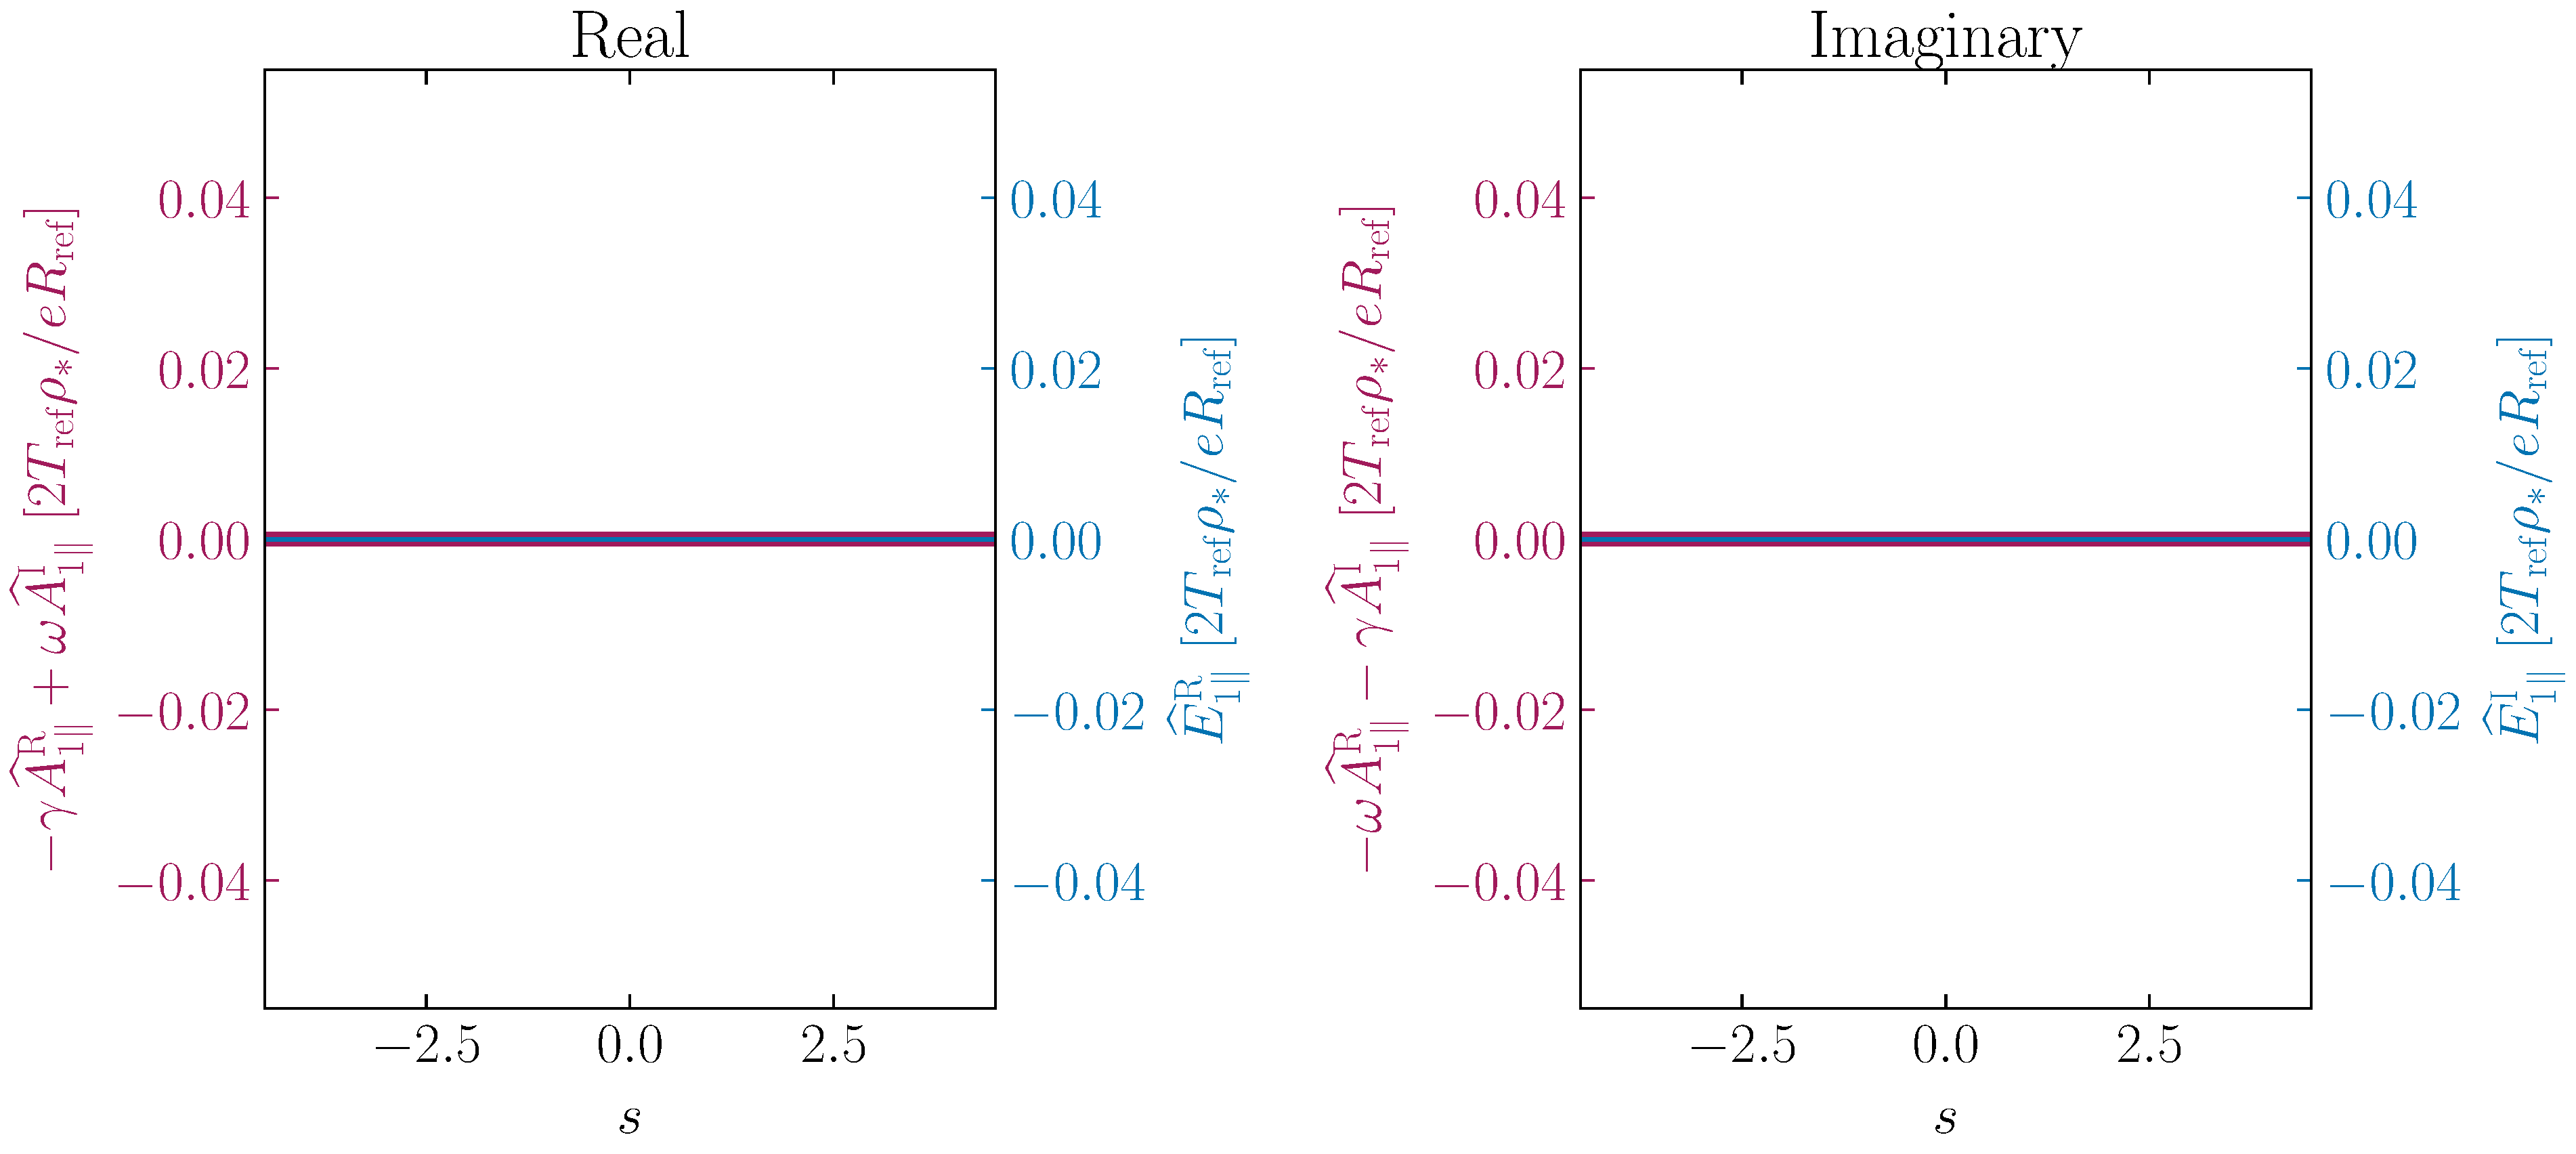
\includegraphics[width=0.9\textwidth]{evaluation/benchmark/g-version/fields/kthrho0.300_beta0.000_fields_g-version.pdf} \\
        $ \beta = 0.2\,\%$ \\
        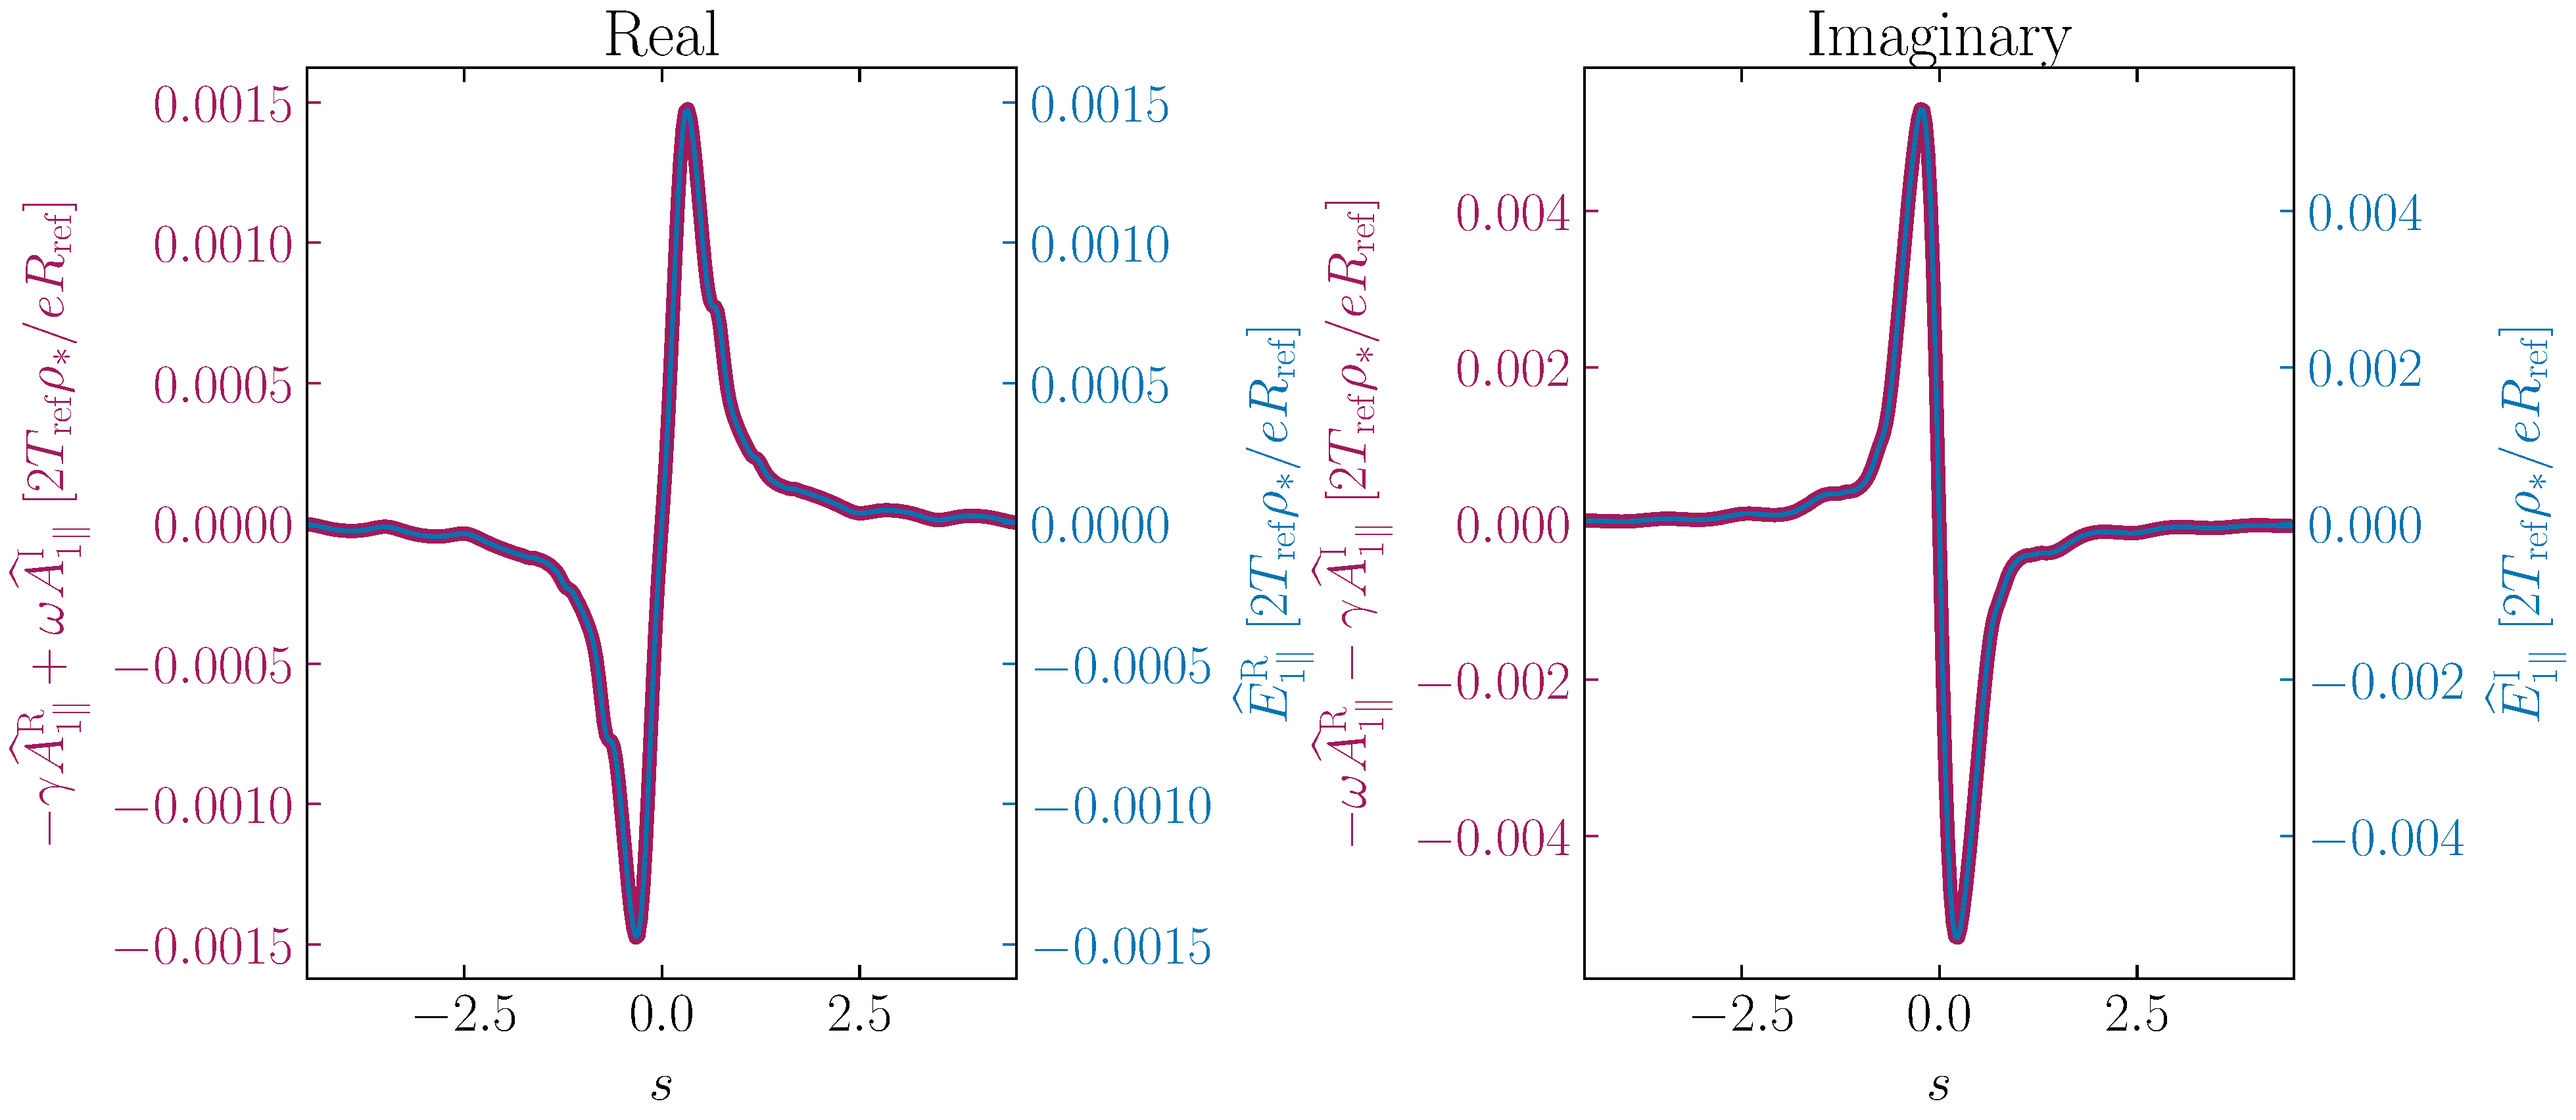
\includegraphics[width=0.9\textwidth]{evaluation/benchmark/g-version/fields/kthrho0.300_beta0.002_fields_g-version.pdf} \\
        $ \beta = 0.4\,\%$ \\
        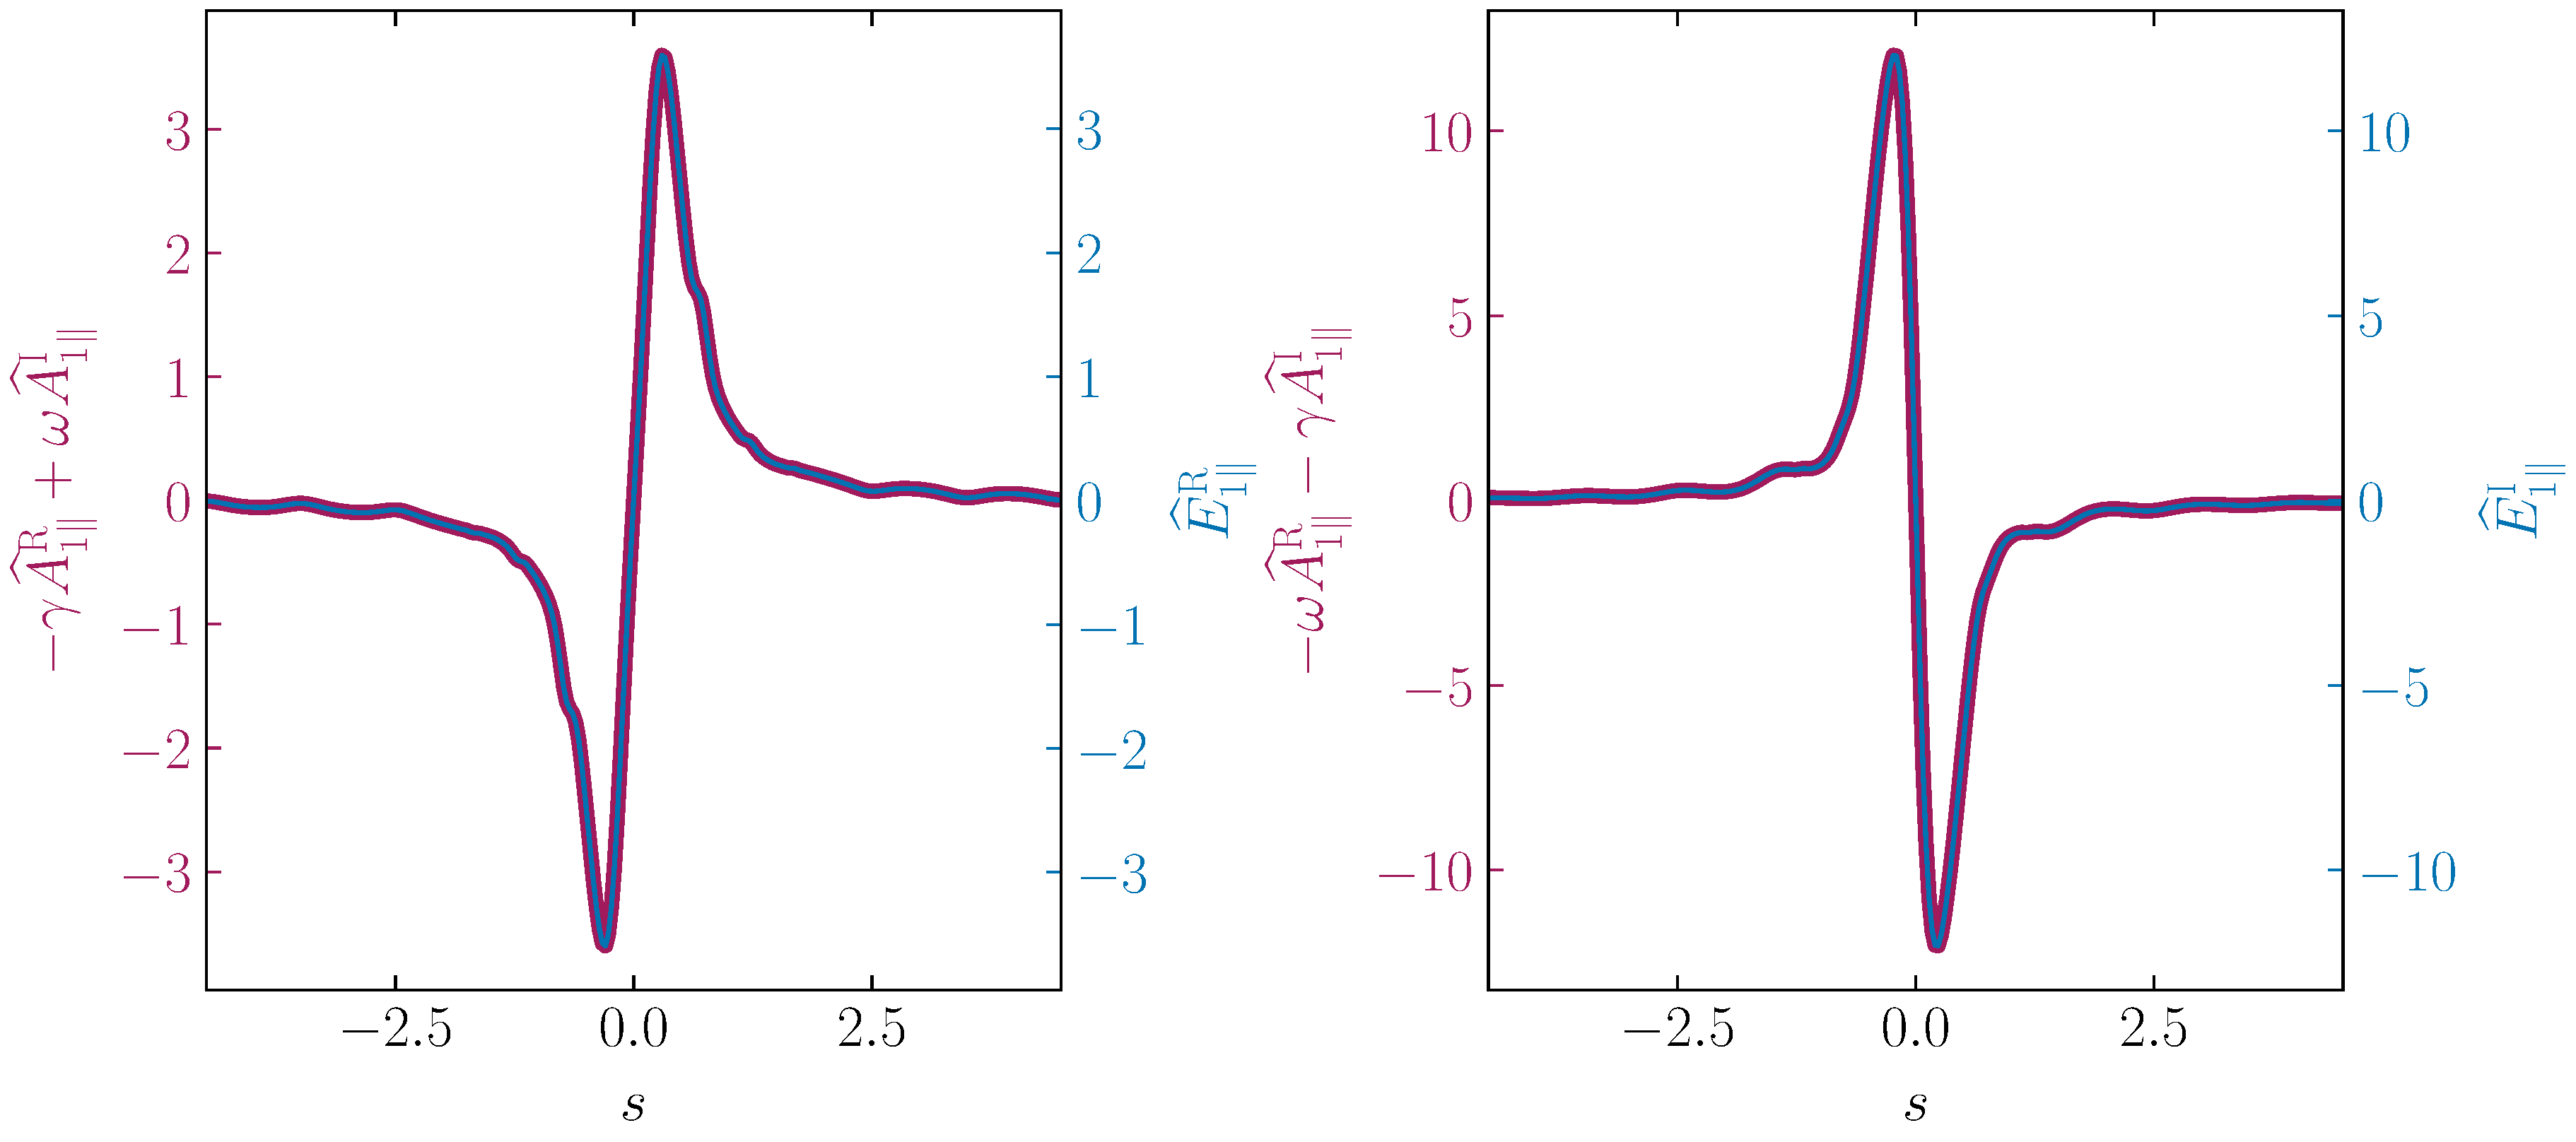
\includegraphics[width=0.9\textwidth]{evaluation/benchmark/g-version/fields/kthrho0.300_beta0.004_fields_g-version.pdf} \\
    \end{tabular}
    % \captionof{figure}{Comparision between real and imaginary part of the induced electric field $\Epar$ and plasma Induction $\Apar$ for various plasma beta $\beta$ for the g-version of {\gkw}}
    % \label{fig:fieldComparisionGVersionAll}
\end{center}

\begin{center}
    % \captionsetup{type=figure}
    \begin{tabular}{c}
        $ \beta = 0.6\,\%$ \\
        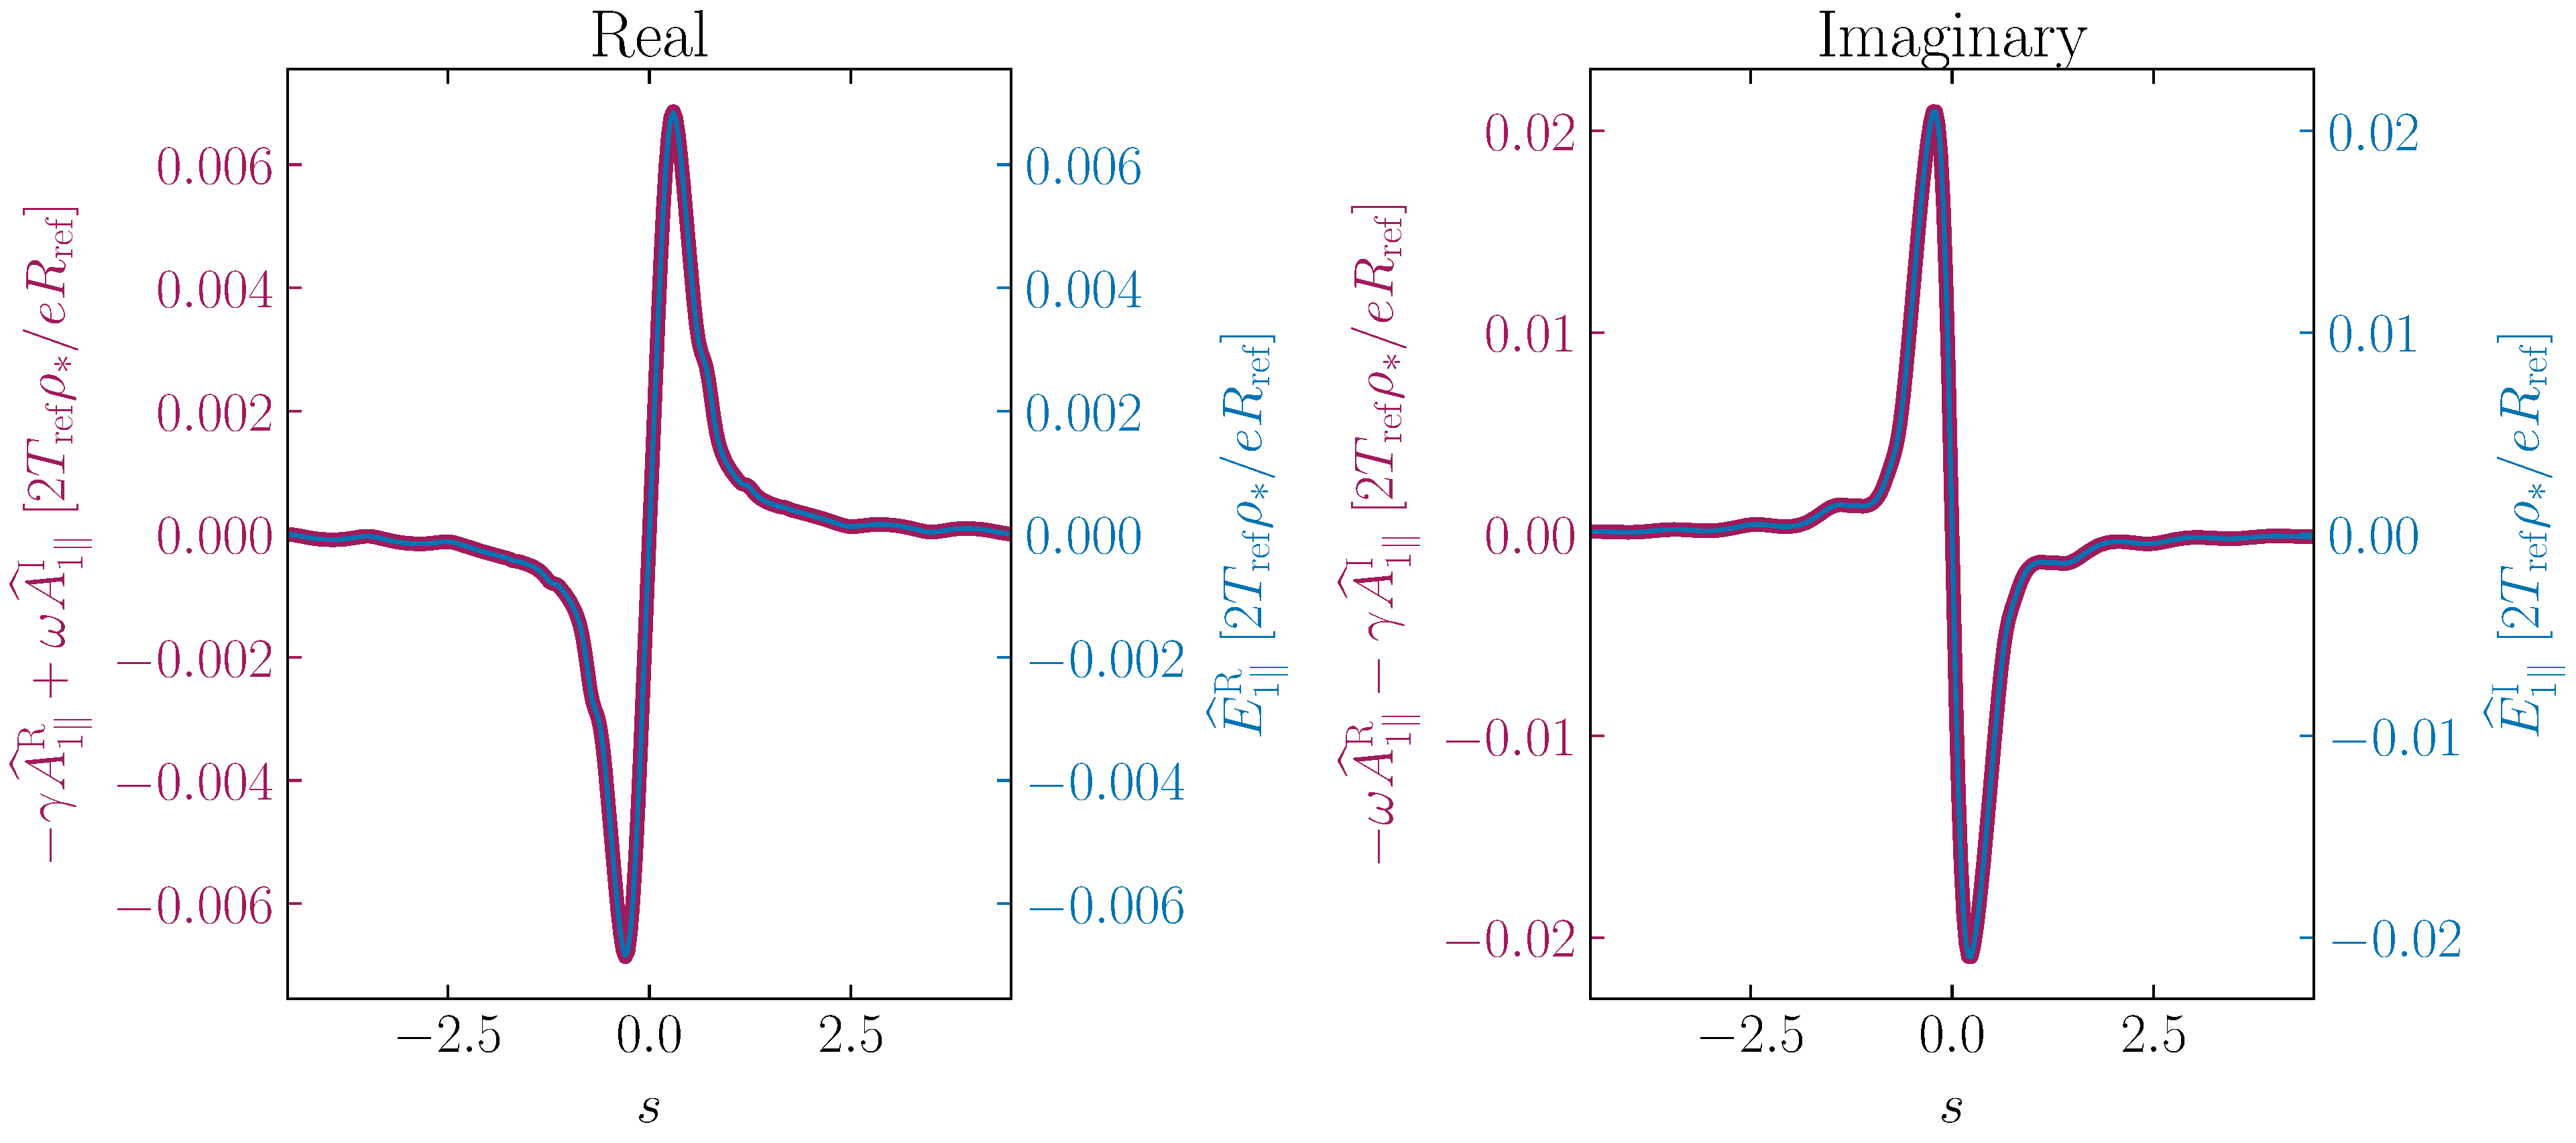
\includegraphics[width=0.9\textwidth]{evaluation/benchmark/g-version/fields/kthrho0.300_beta0.006_fields_g-version.pdf} \\
        $ \beta = 0.8\,\%$ \\
        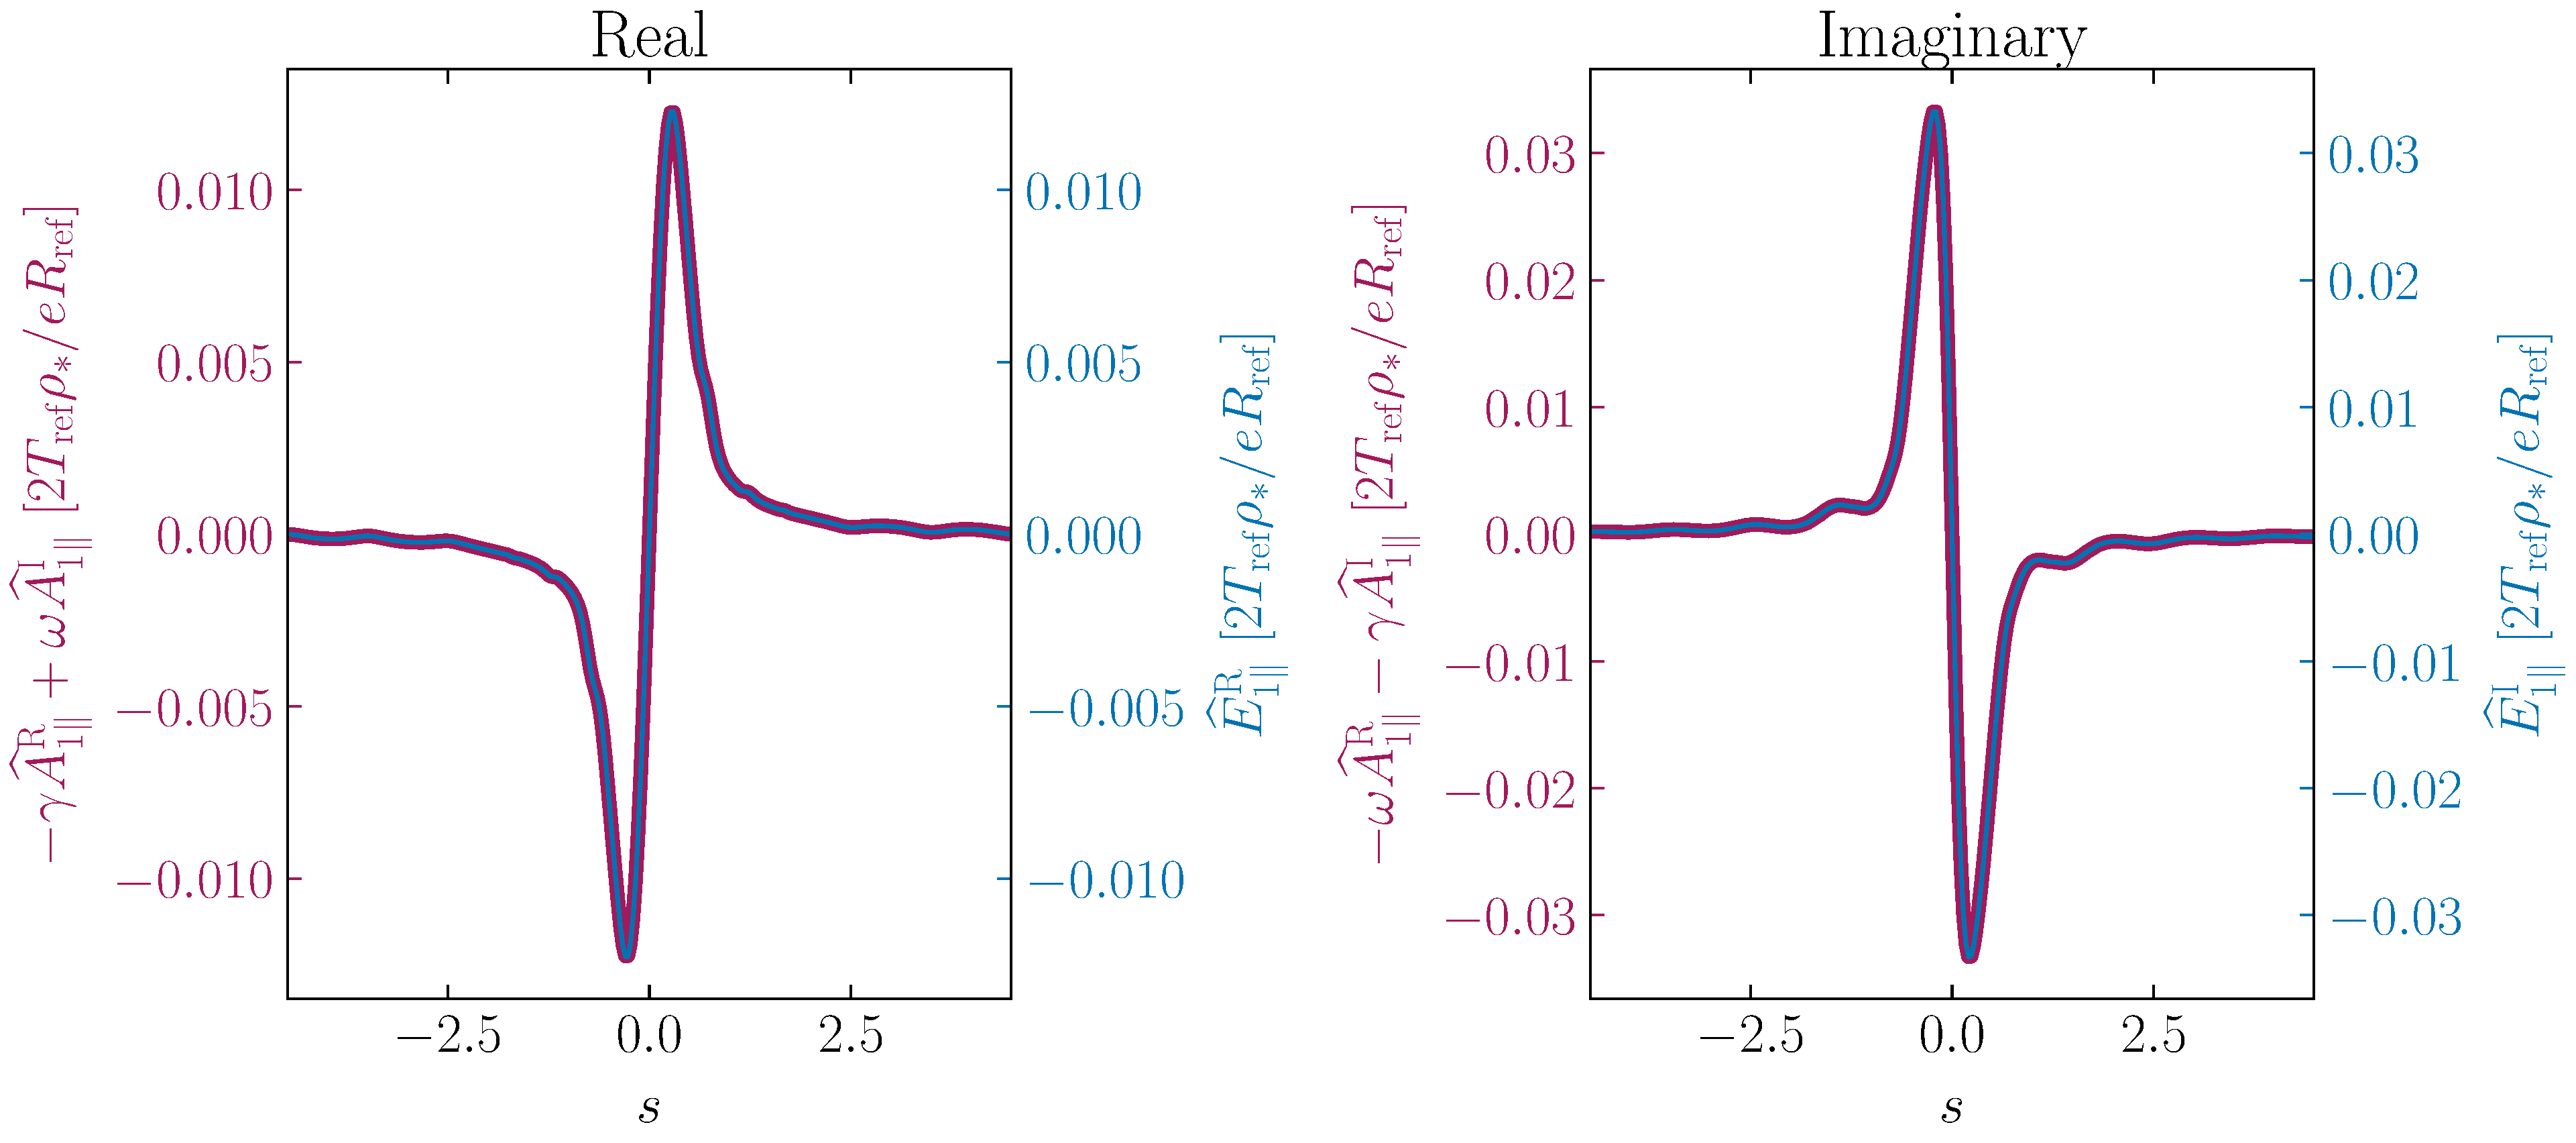
\includegraphics[width=0.9\textwidth]{evaluation/benchmark/g-version/fields/kthrho0.300_beta0.008_fields_g-version.pdf} \\
        $ \beta = 1.0\,\%$ \\
        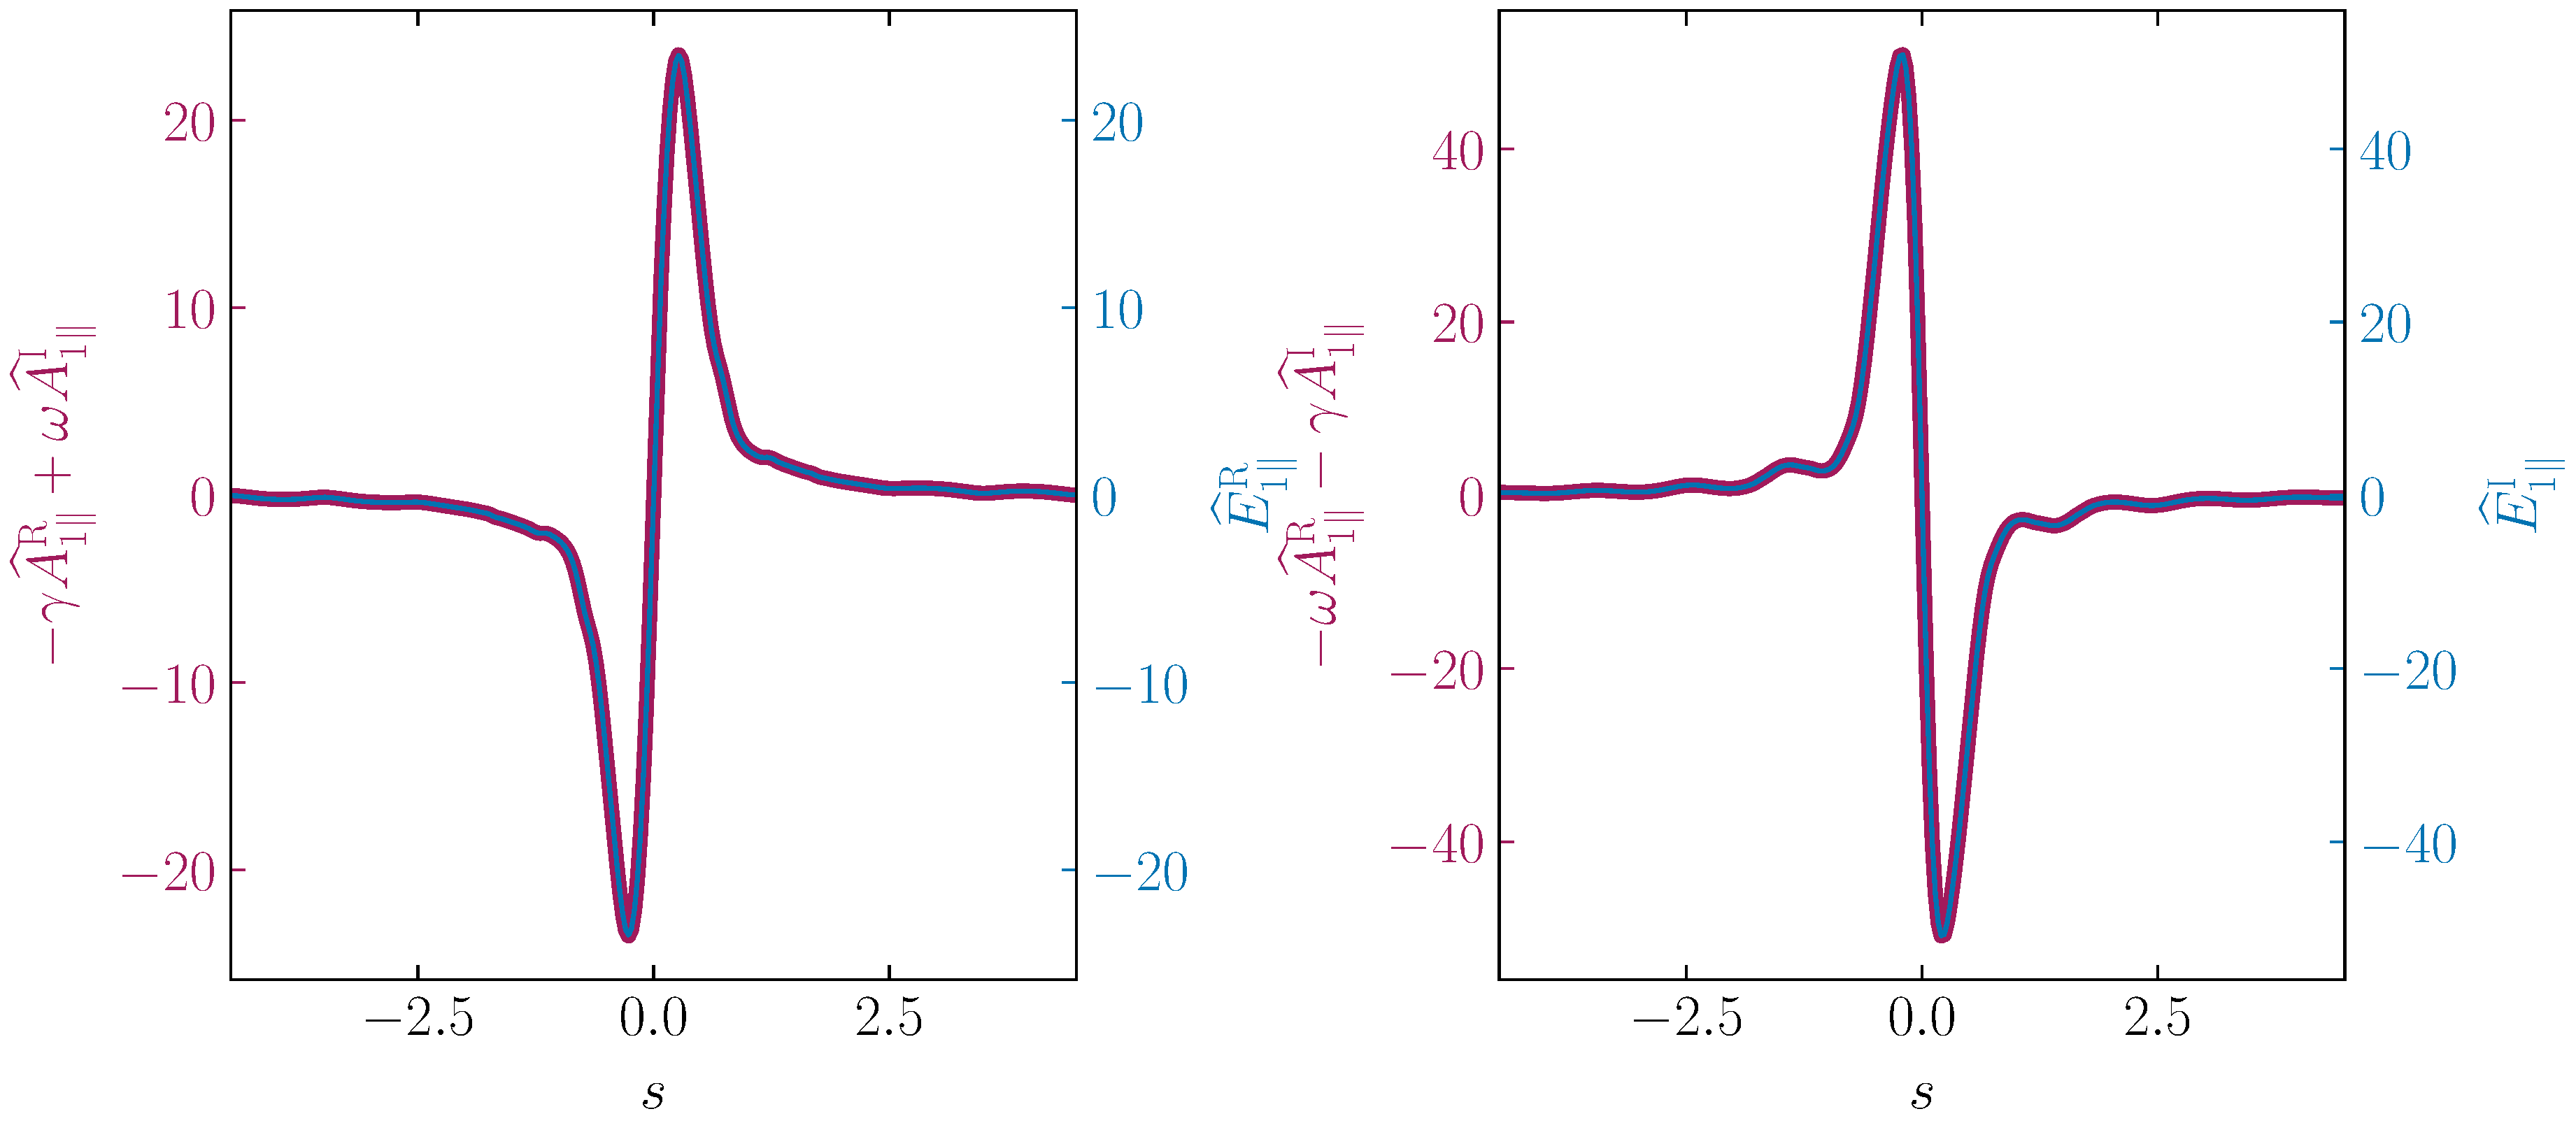
\includegraphics[width=0.9\textwidth]{evaluation/benchmark/g-version/fields/kthrho0.300_beta0.010_fields_g-version.pdf} \\
    \end{tabular}
    % \captionof{figure}{Comparision between real and imaginary part of the induced electric field $\Epar$ and plasma Induction $\Apar$ for various plasma beta $\beta$ for the g-version of {\gkw}}
    % \label{fig:fieldComparisionGVersionAll}
\end{center}

\begin{center}
    % \captionsetup{type=figure}
    \begin{tabular}{c}
        $ \beta = 1.1\,\%$ \\
        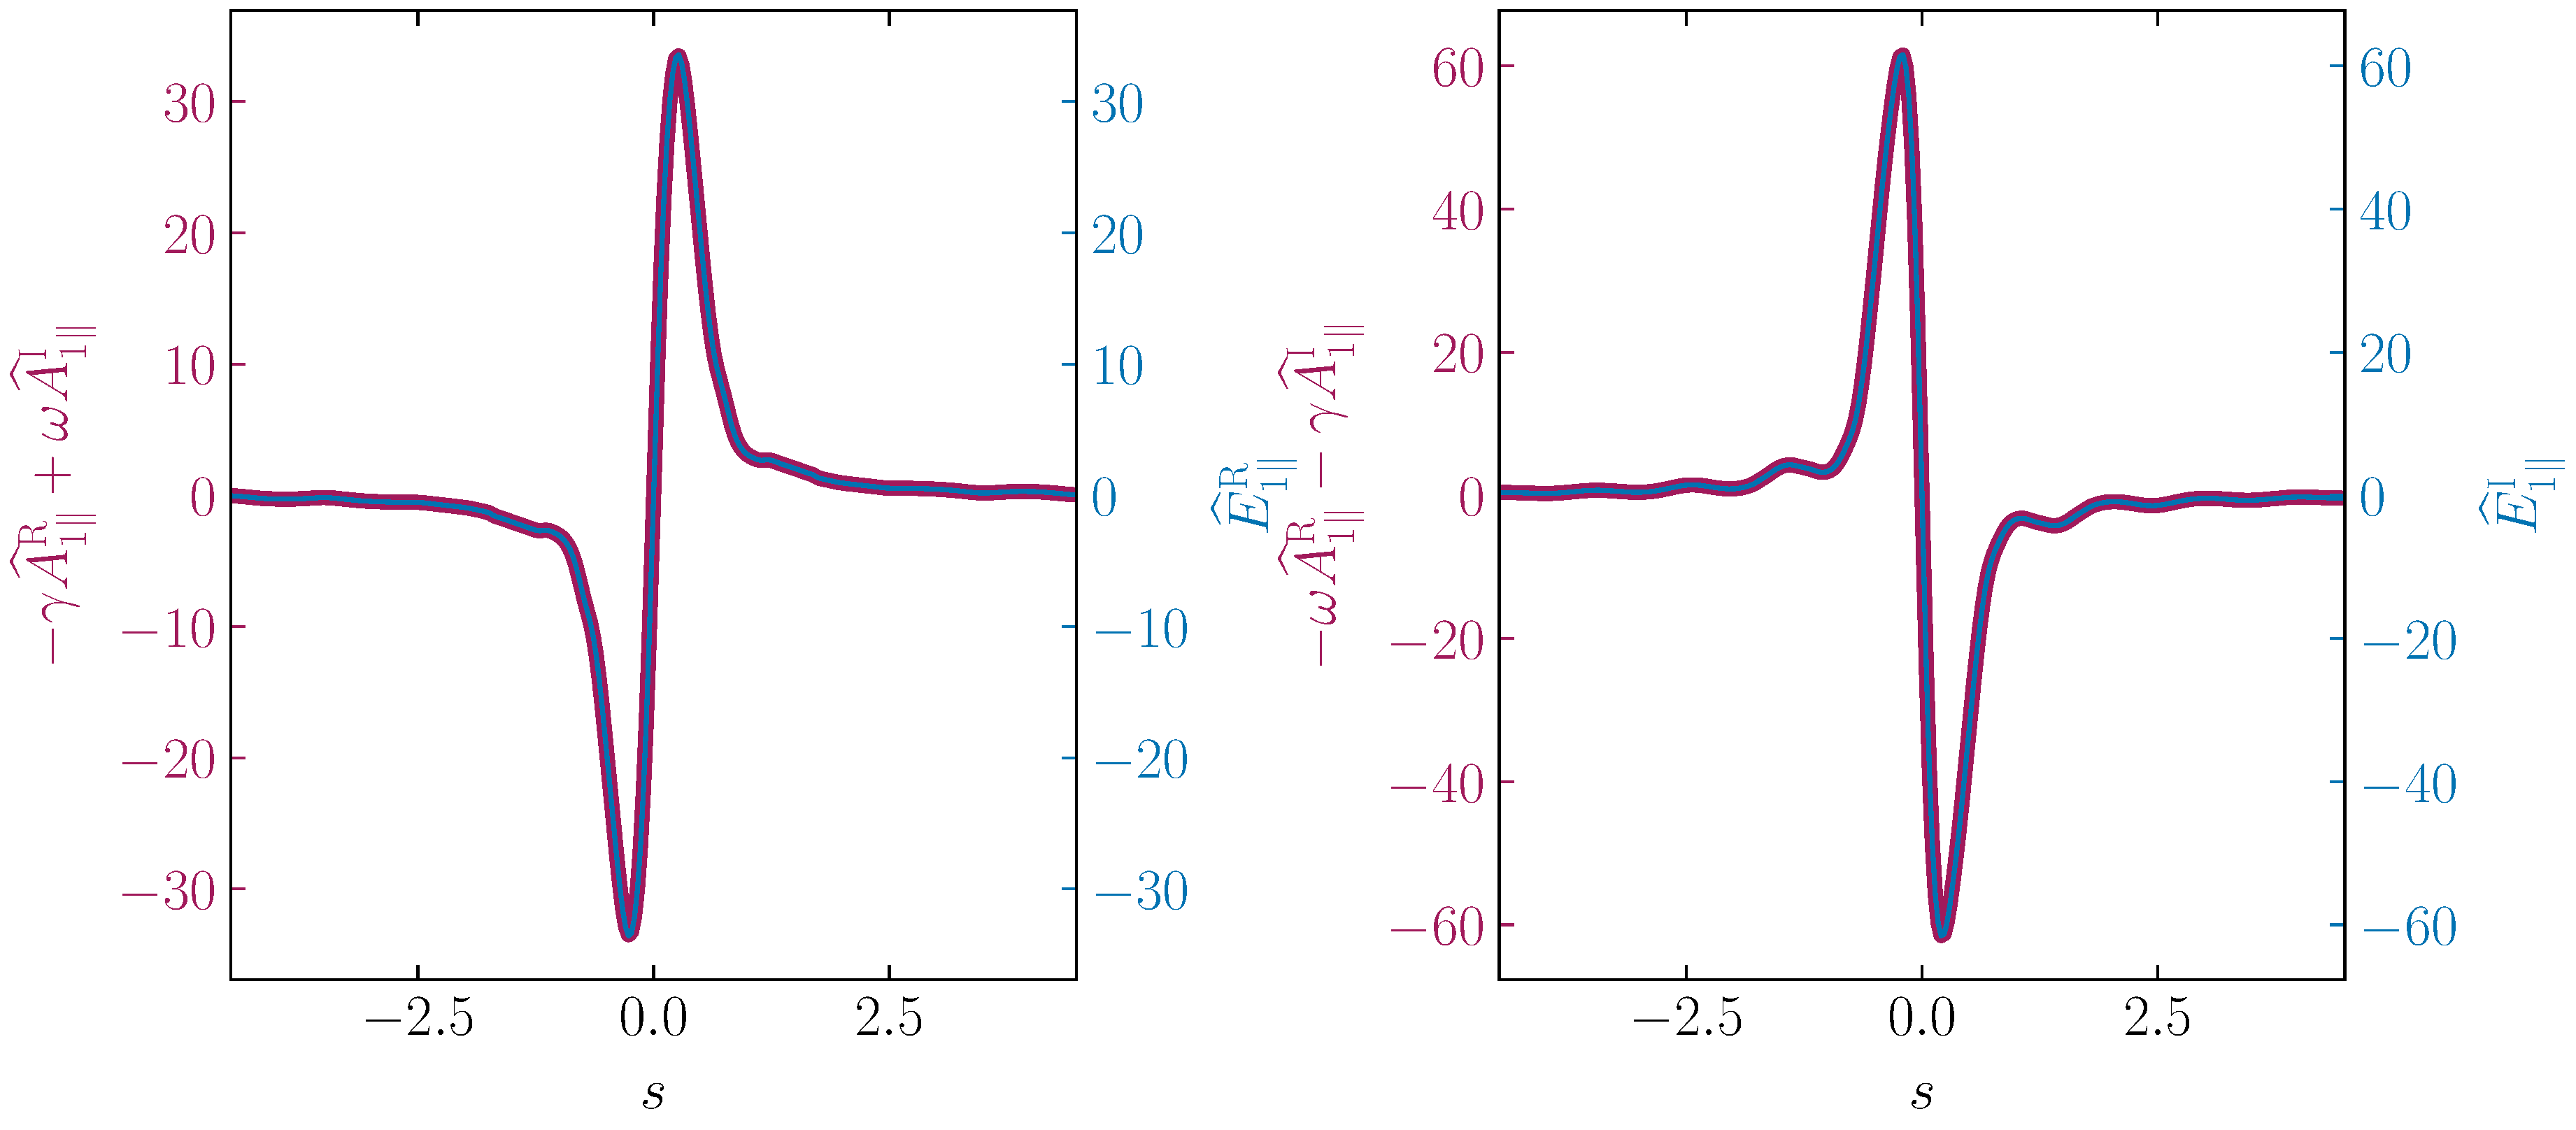
\includegraphics[width=0.9\textwidth]{evaluation/benchmark/g-version/fields/kthrho0.300_beta0.011_fields_g-version.pdf} \\
        $ \beta = 1.2\,\%$ \\
        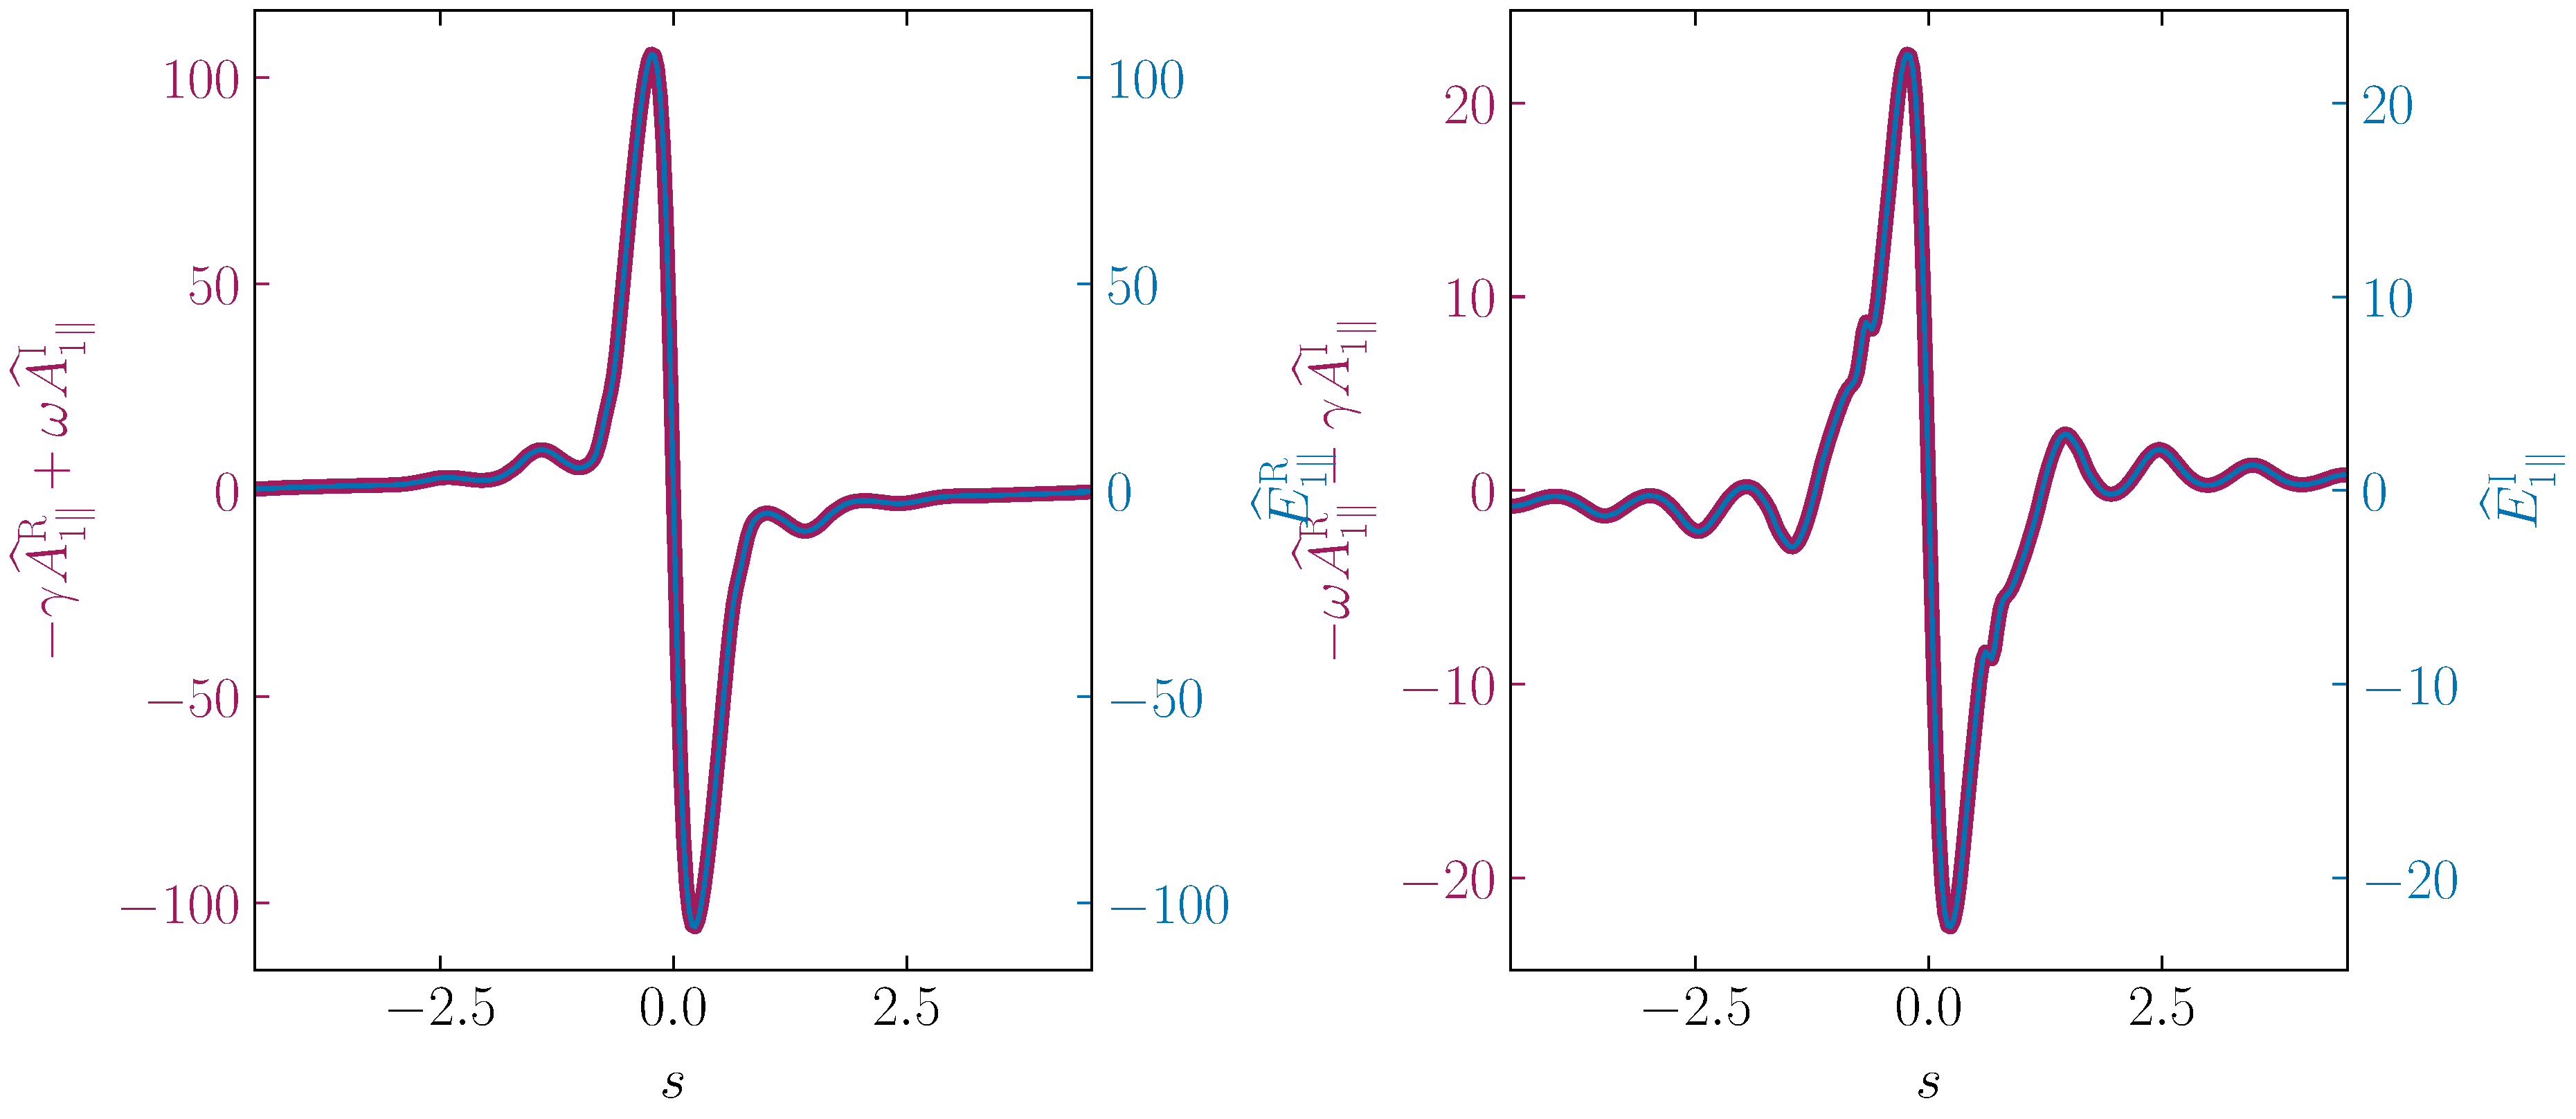
\includegraphics[width=0.9\textwidth]{evaluation/benchmark/g-version/fields/kthrho0.300_beta0.012_fields_g-version.pdf} \\
        $ \beta = 1.4\,\%$ \\
        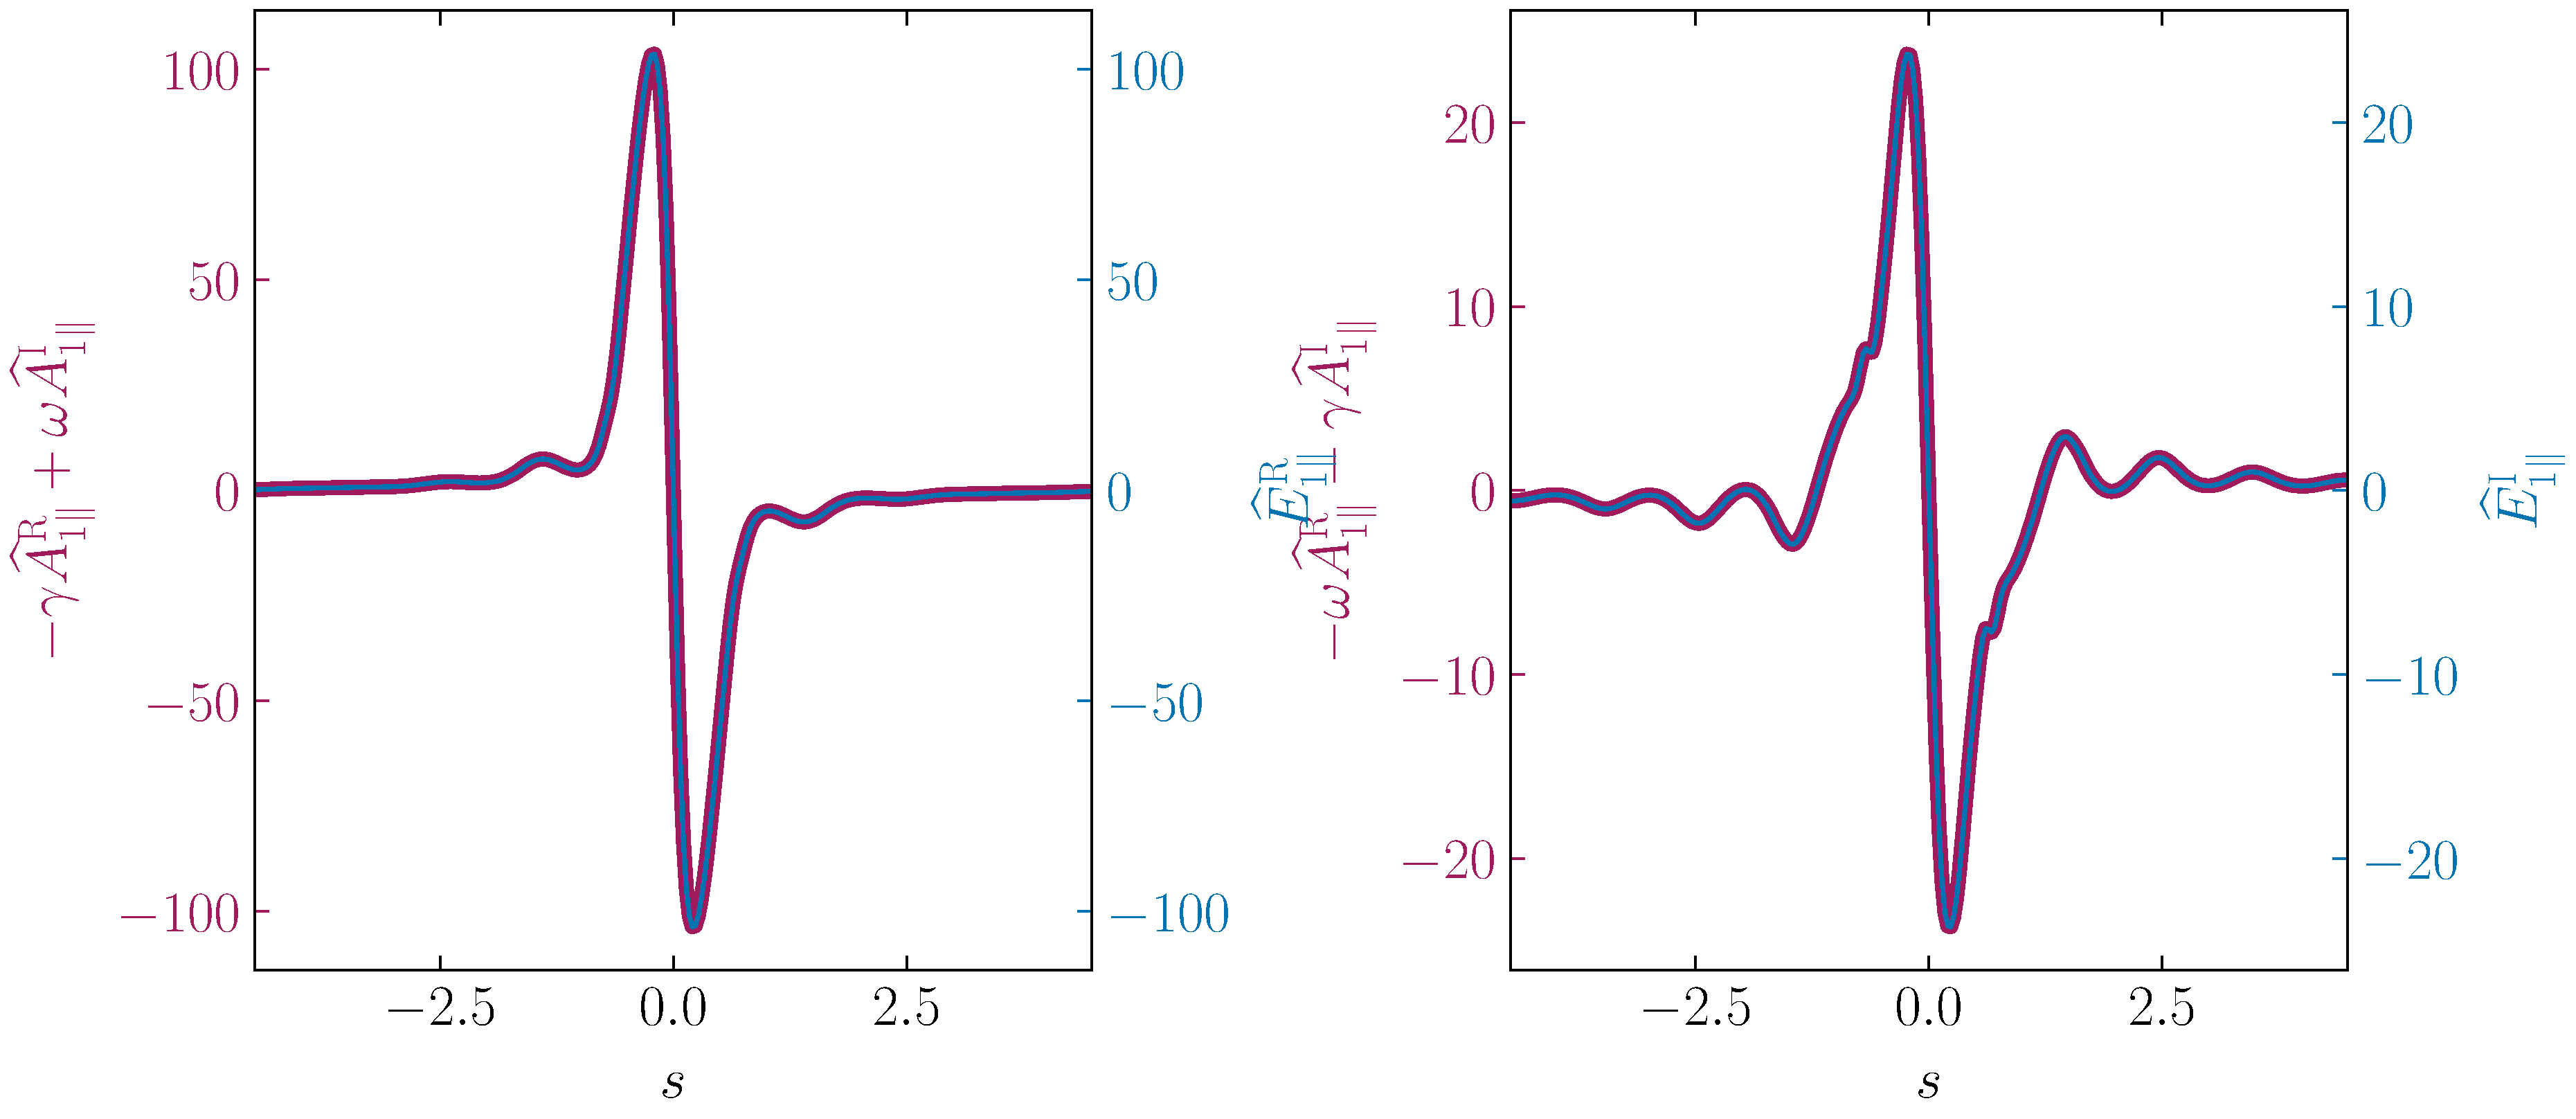
\includegraphics[width=0.9\textwidth]{evaluation/benchmark/g-version/fields/kthrho0.300_beta0.014_fields_g-version.pdf} \\
    \end{tabular}
    % \captionof{figure}{Comparision between real and imaginary part of the induced electric field $\Epar$ and plasma Induction $\Apar$ for various plasma beta $\beta$ for the g-version of {\gkw}}
    % \label{fig:fieldComparisionGVersionAll}
\end{center}

\begin{center}
    % \captionsetup{type=figure}
    \begin{tabular}{c}
        $ \beta = 1.6\,\%$ \\
        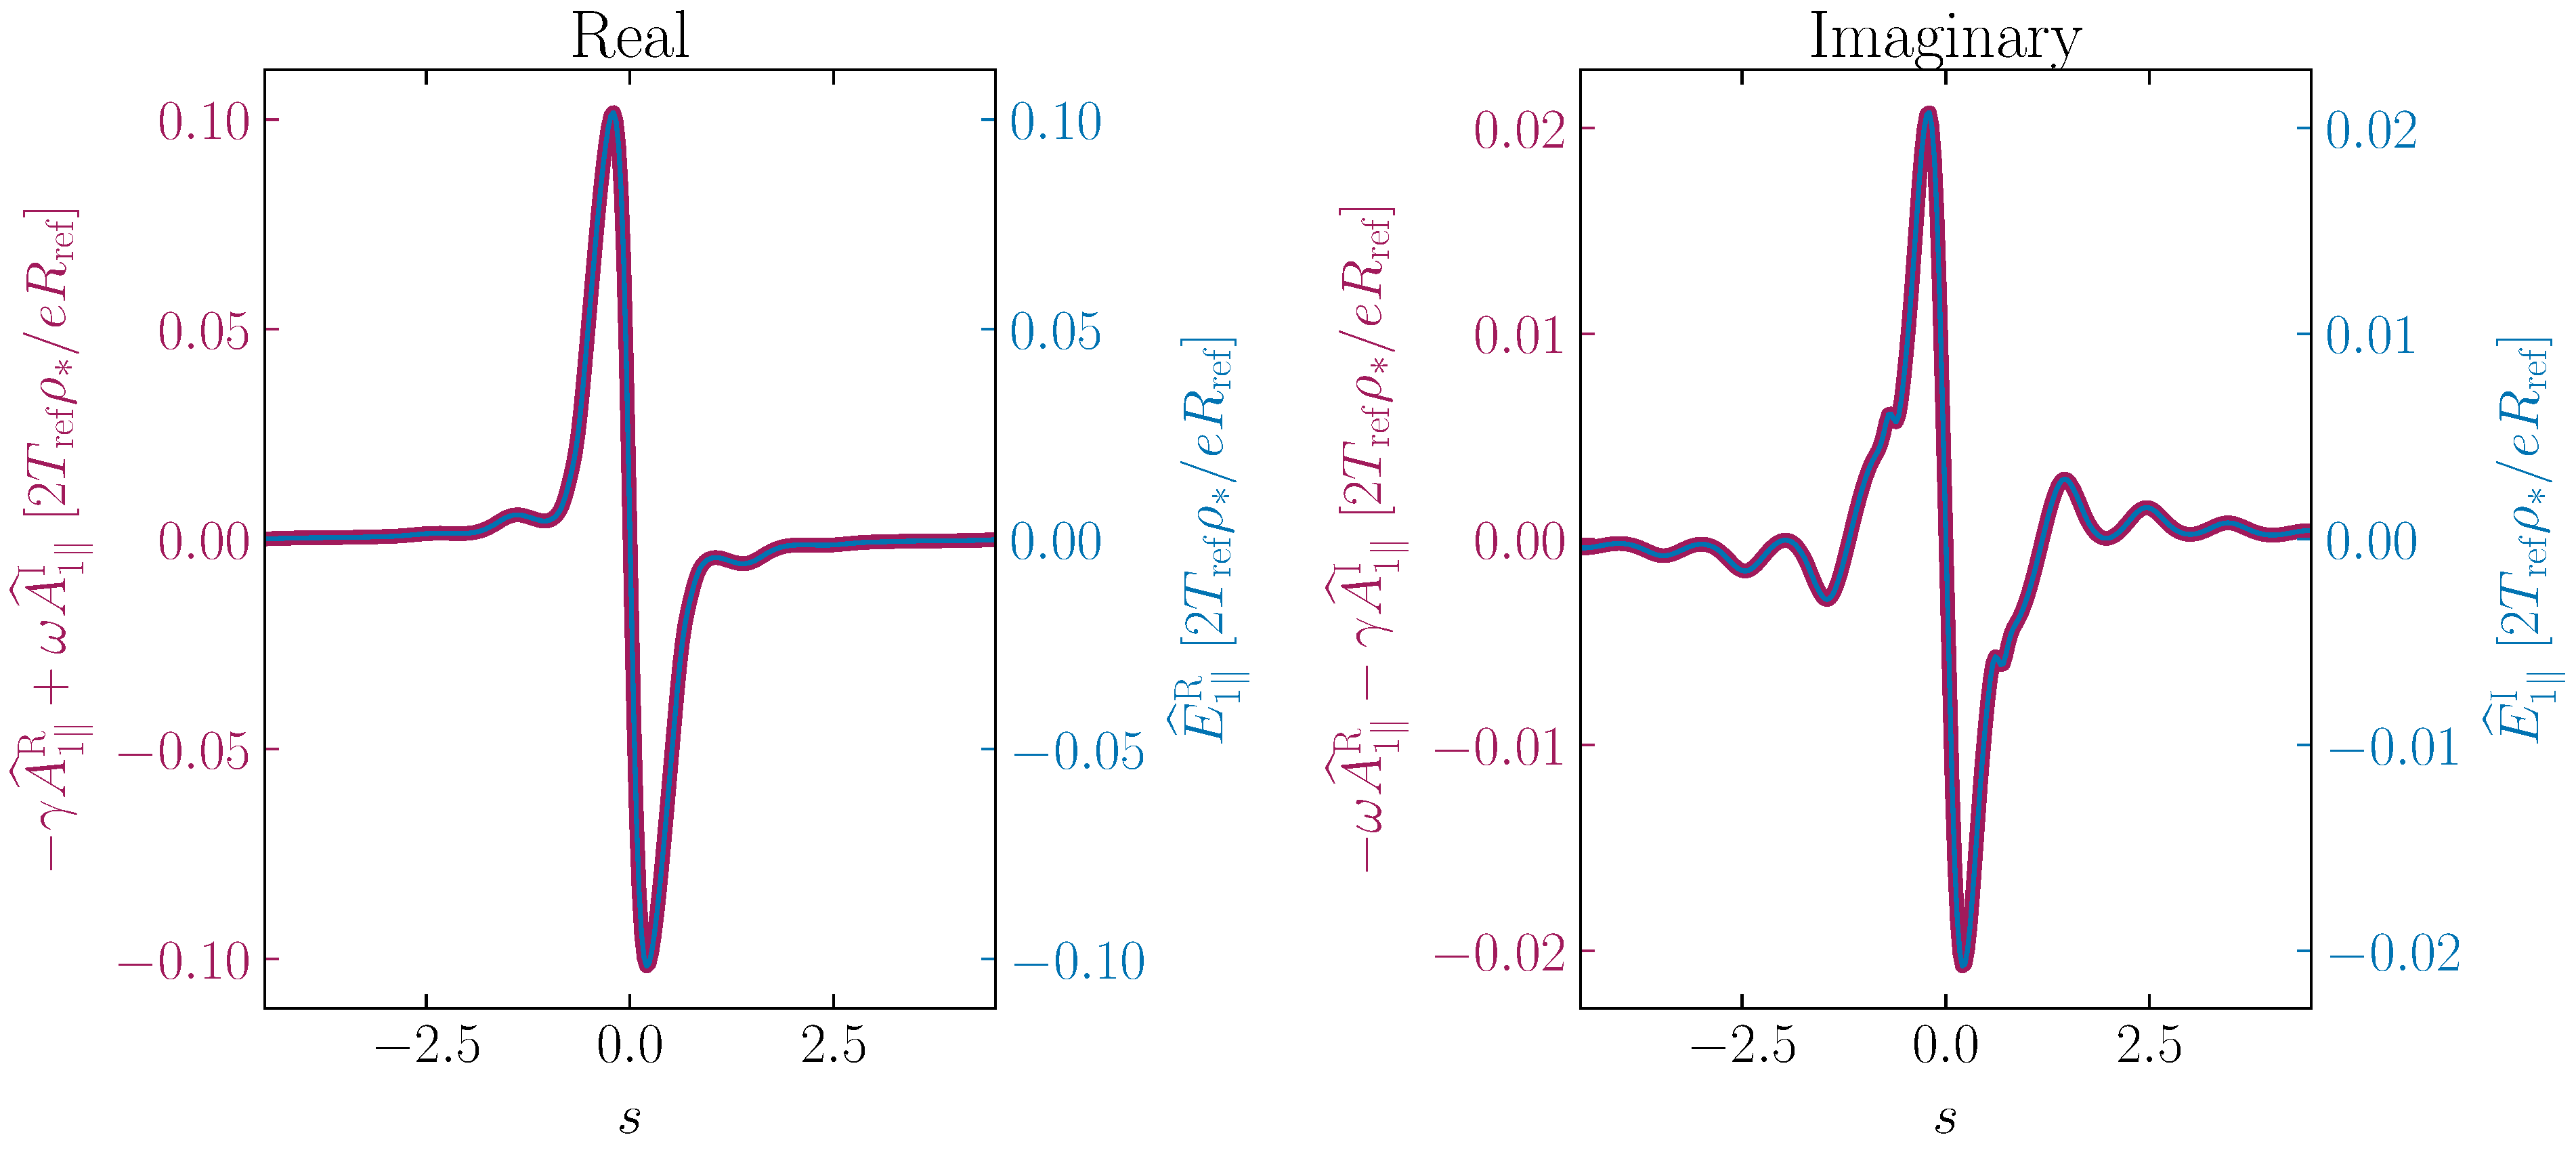
\includegraphics[width=0.9\textwidth]{evaluation/benchmark/g-version/fields/kthrho0.300_beta0.016_fields_g-version.pdf} \\
    \end{tabular}
    % \captionof{figure}{Comparision between real and imaginary part of the induced electric field $\Epar$ and plasma Induction $\Apar$ for various plasma beta $\beta$ for the g-version of {\gkw}}
    % \label{fig:fieldComparisionGVersionAll}
\end{center}

\newpage

\subsection{For the f-version of {\gkw}}
\label{subappend:fieldComparisionFVersion}

\begin{center}
    % \captionsetup{type=figure}
    \begin{tabular}{c}
        $ \beta = 0.0\,\%$ \\
        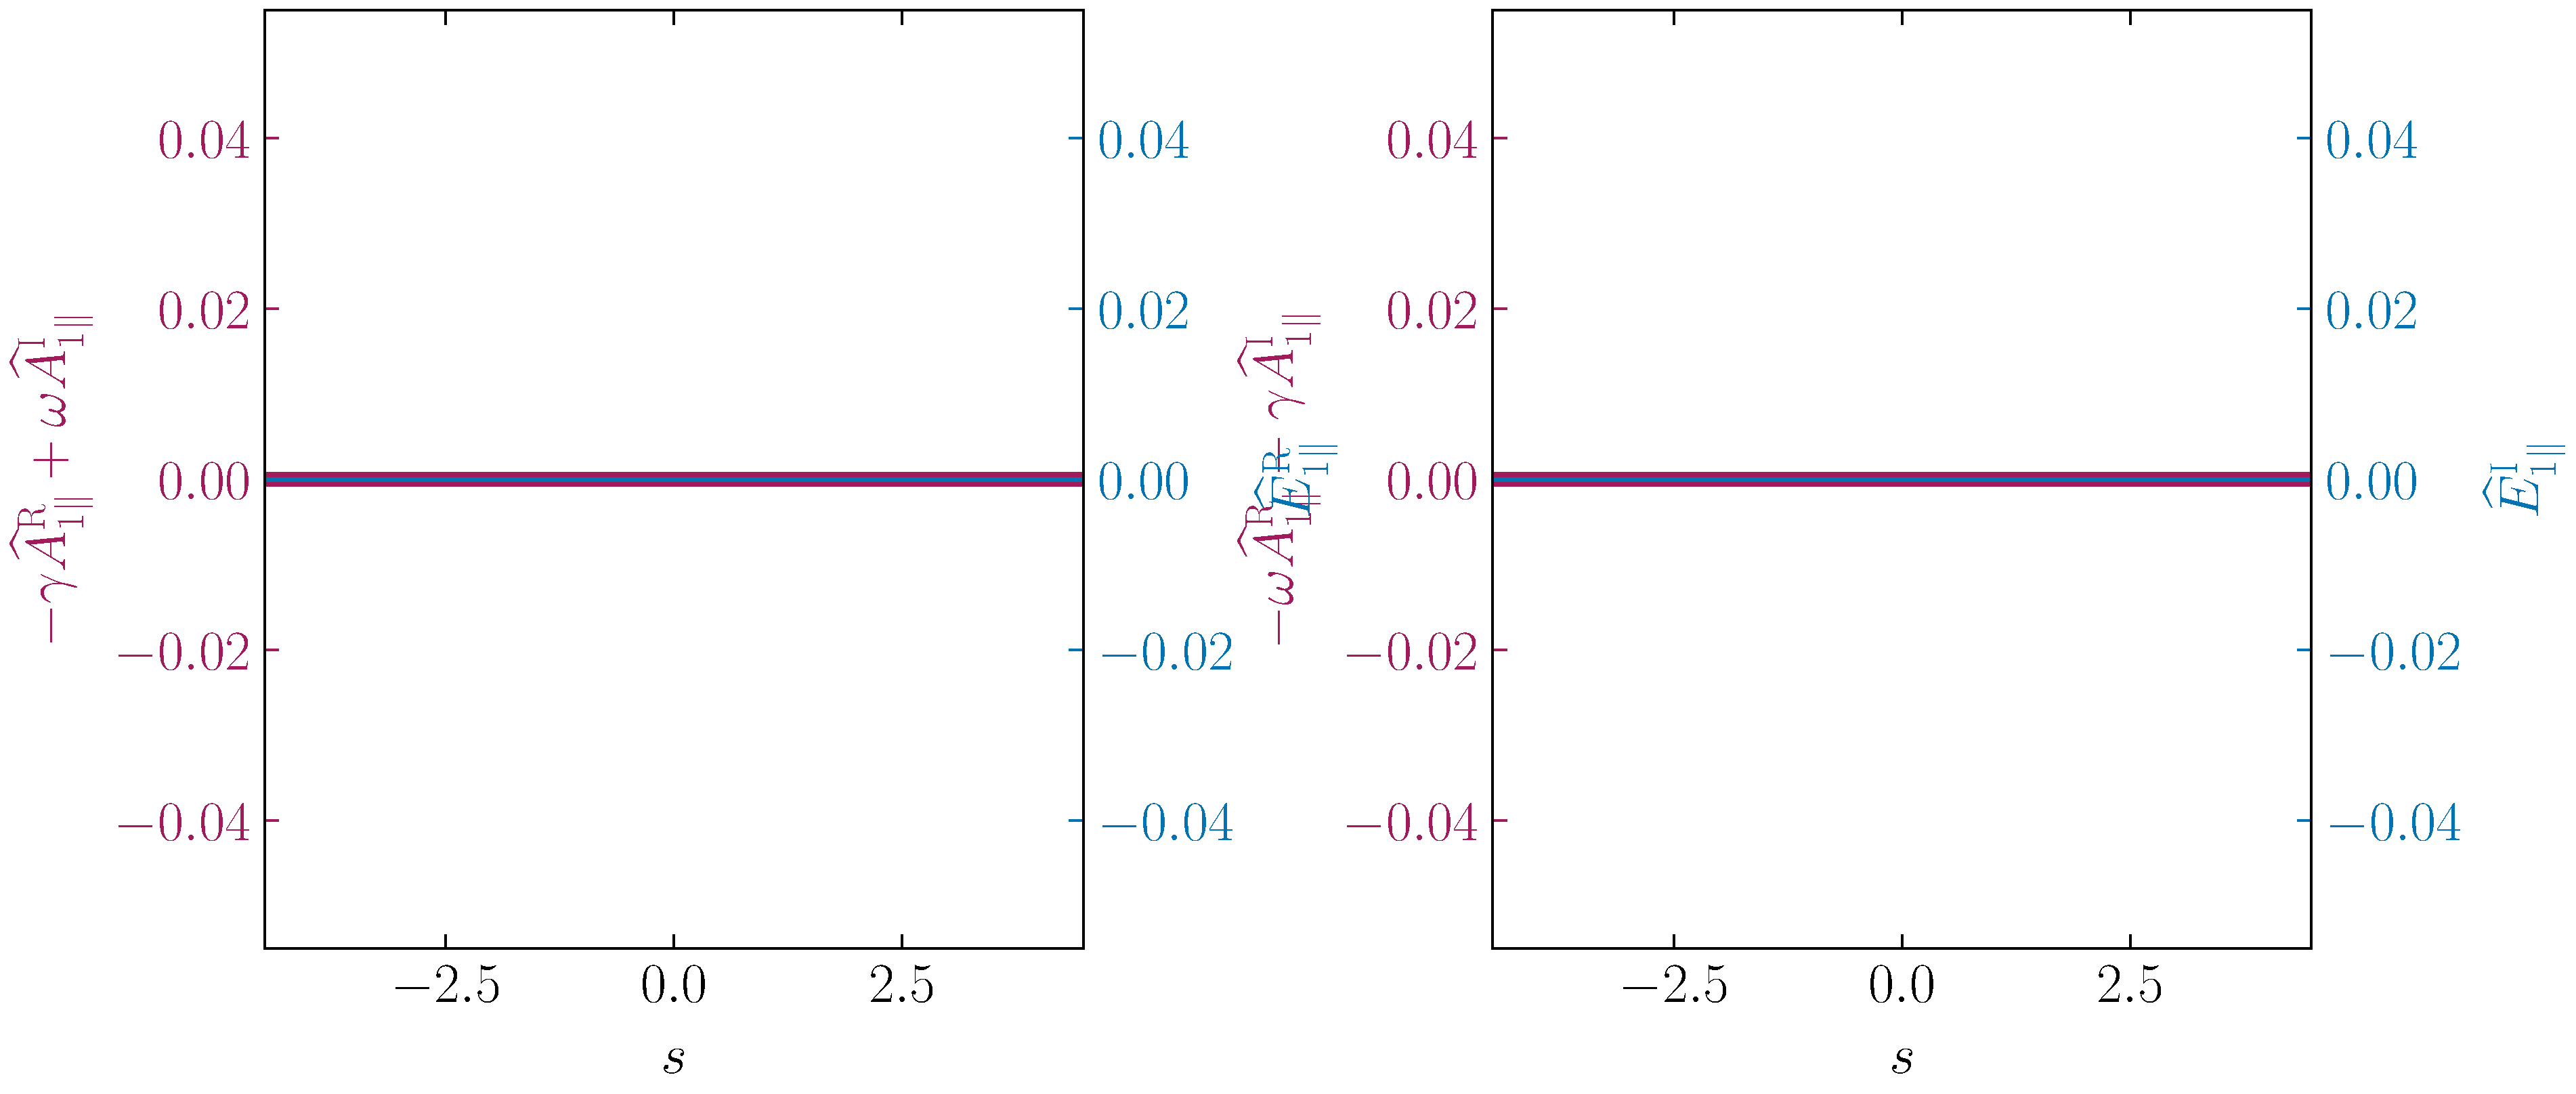
\includegraphics[width=0.9\textwidth]{evaluation/benchmark/f-version/fields/kthrho0.300_beta0.000_fields_f-version.pdf} \\
        $ \beta = 0.2\,\%$ \\
        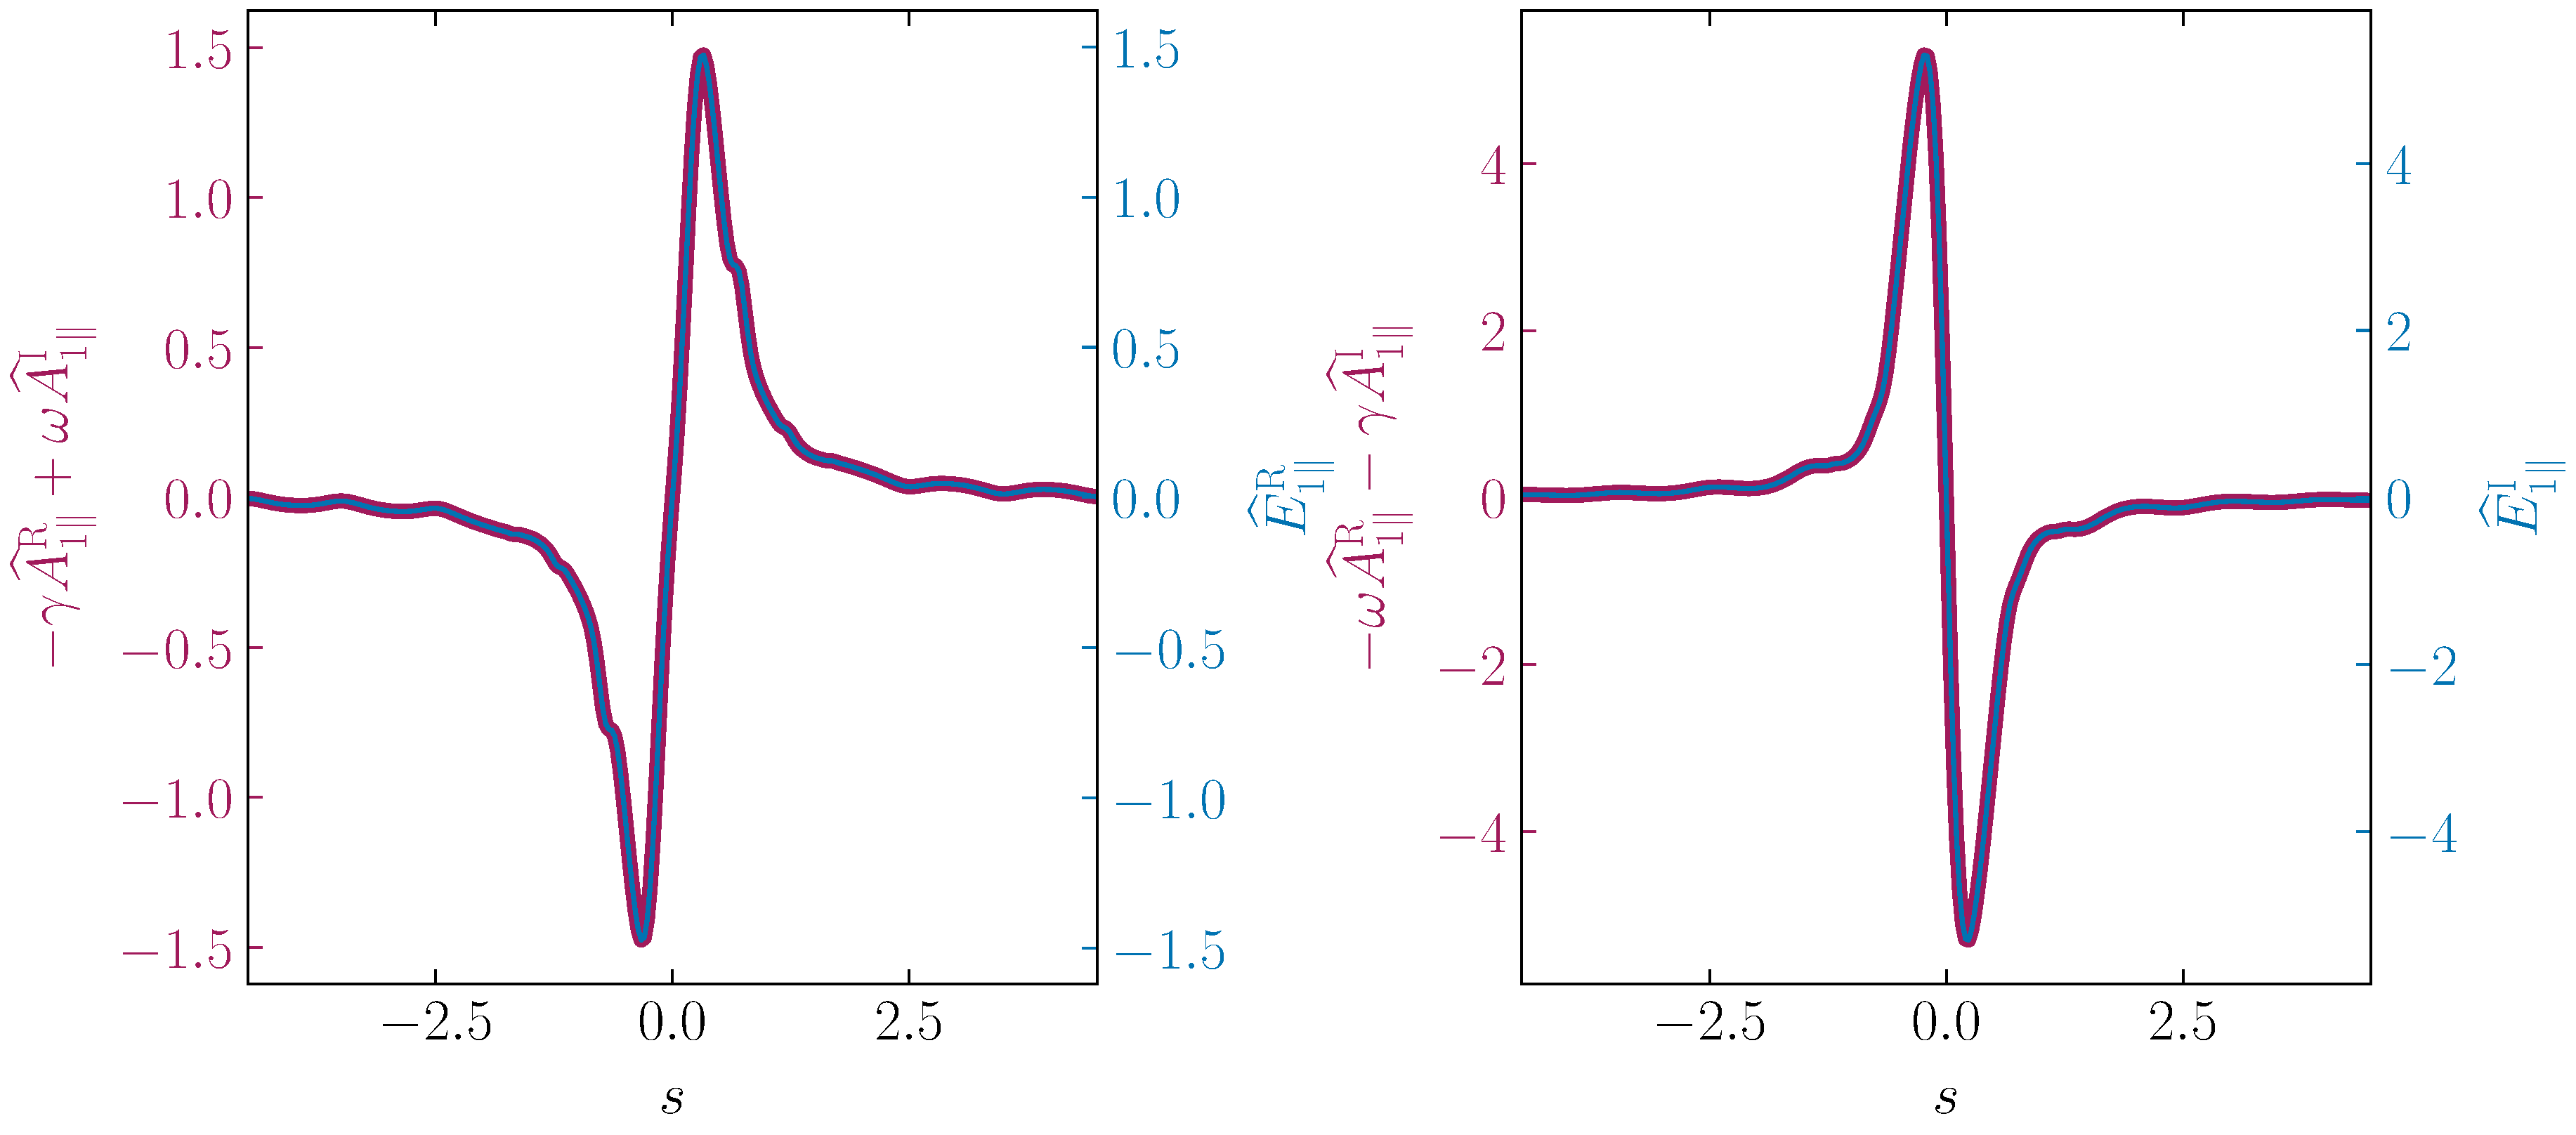
\includegraphics[width=0.9\textwidth]{evaluation/benchmark/f-version/fields/kthrho0.300_beta0.002_fields_f-version.pdf} \\
        $ \beta = 0.4\,\%$ \\
        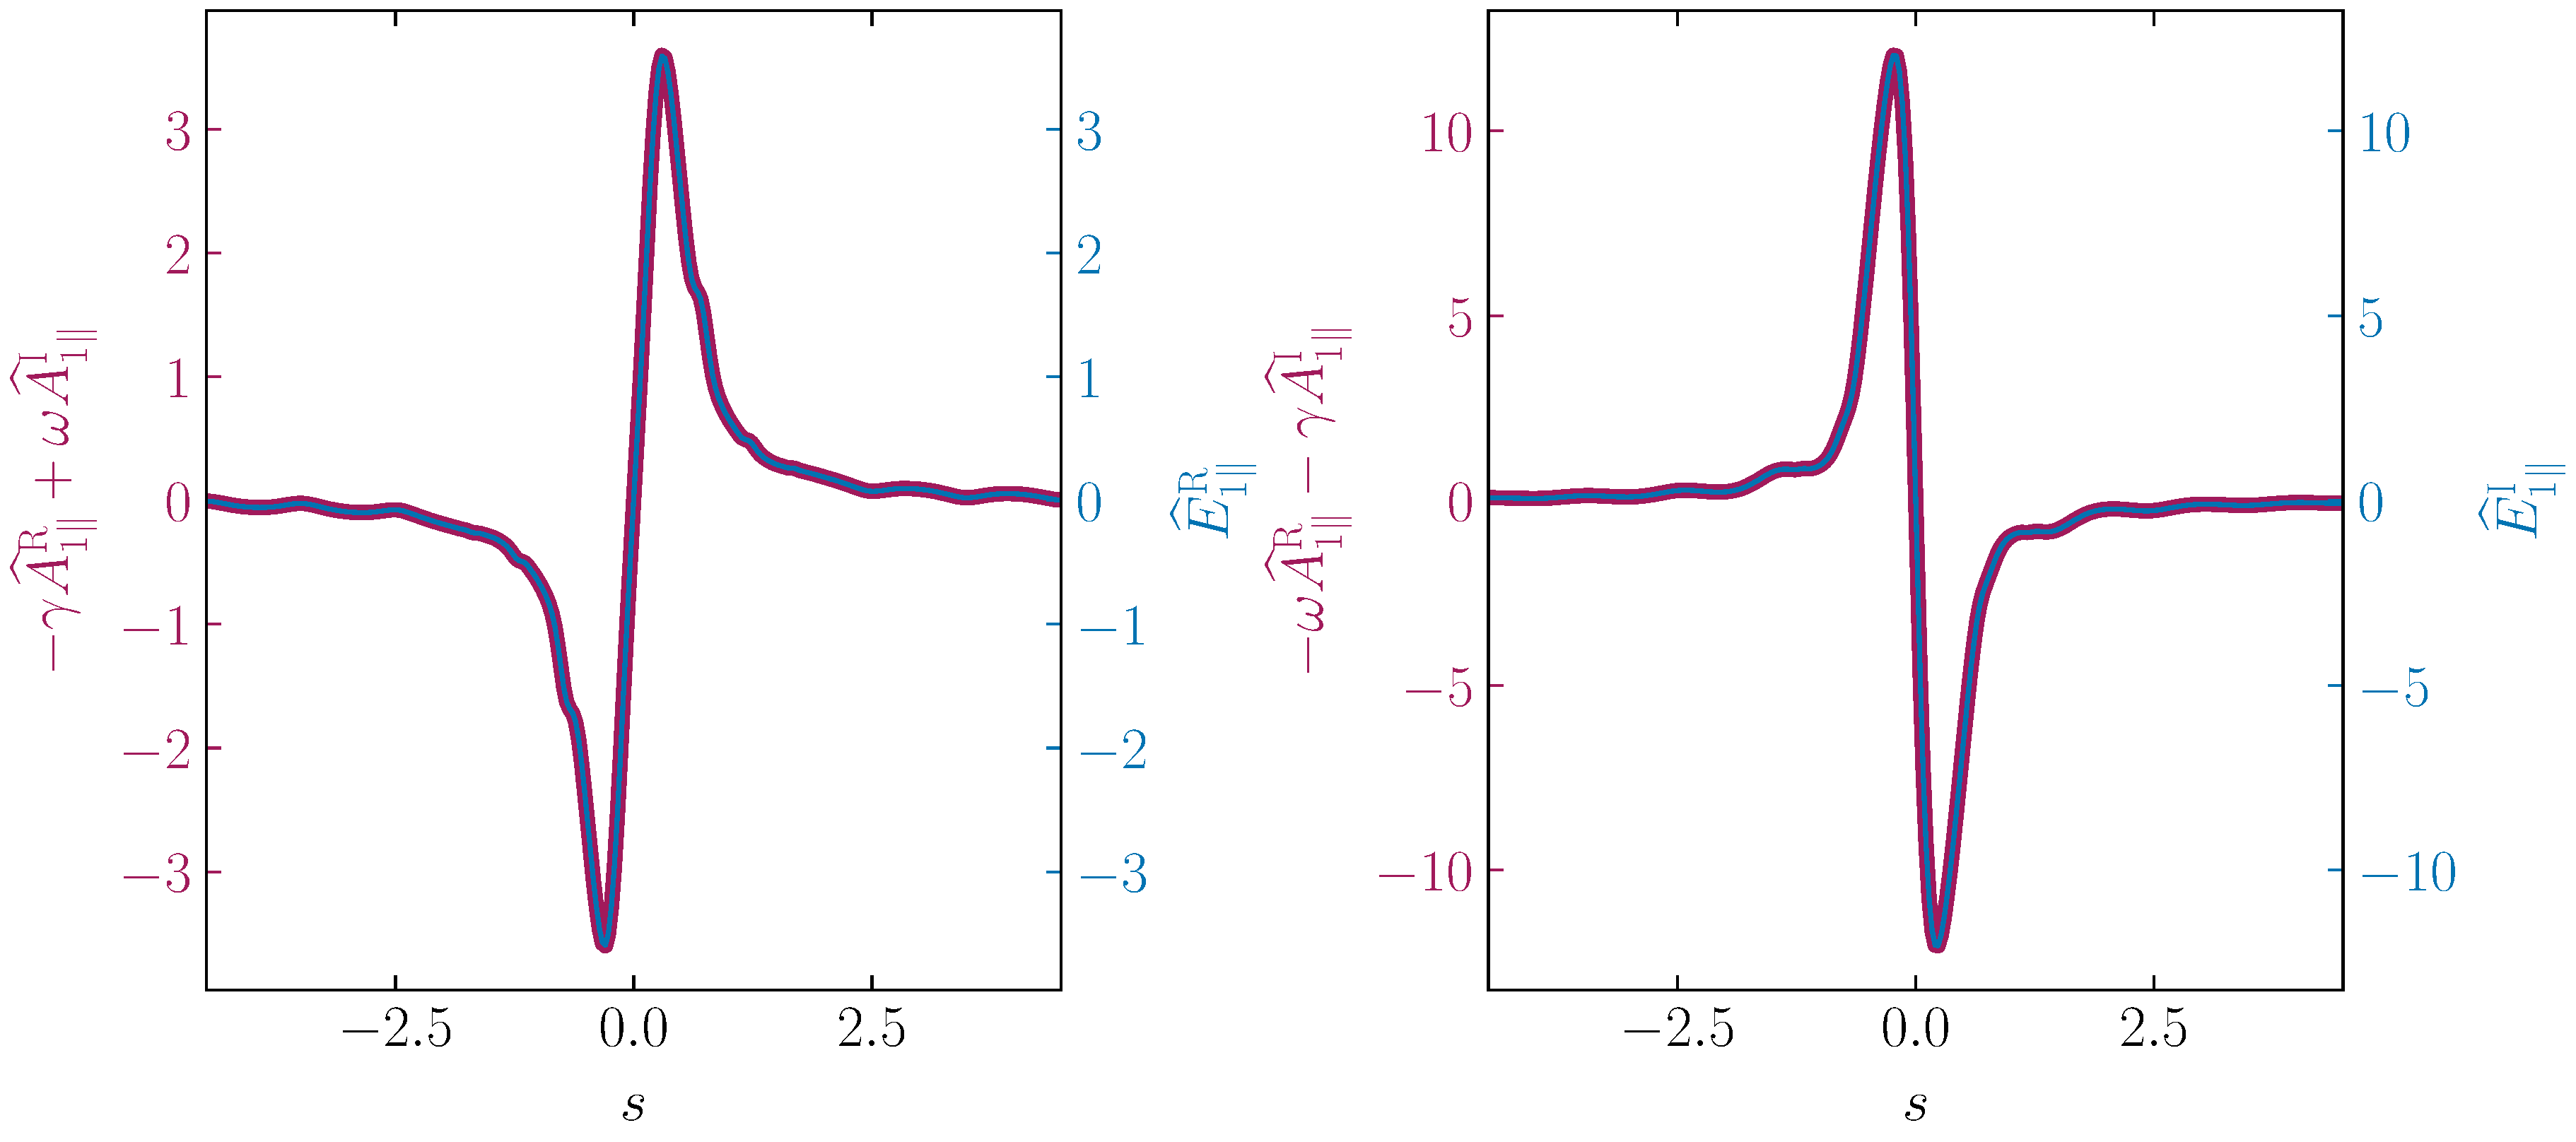
\includegraphics[width=0.9\textwidth]{evaluation/benchmark/f-version/fields/kthrho0.300_beta0.004_fields_f-version.pdf} \\
    \end{tabular}
    % \captionof{figure}{Comparision between real and imaginary part of the induced electric field $\Epar$ and plasma Induction $\Apar$ for various plasma beta $\beta$ for the f-version of {\gkw}}
    % \label{fig:fieldComparisionGVersionAll}
\end{center}

\begin{center}
    % \captionsetup{type=figure}
    \begin{tabular}{c}
        $ \beta = 0.6\,\%$ \\
        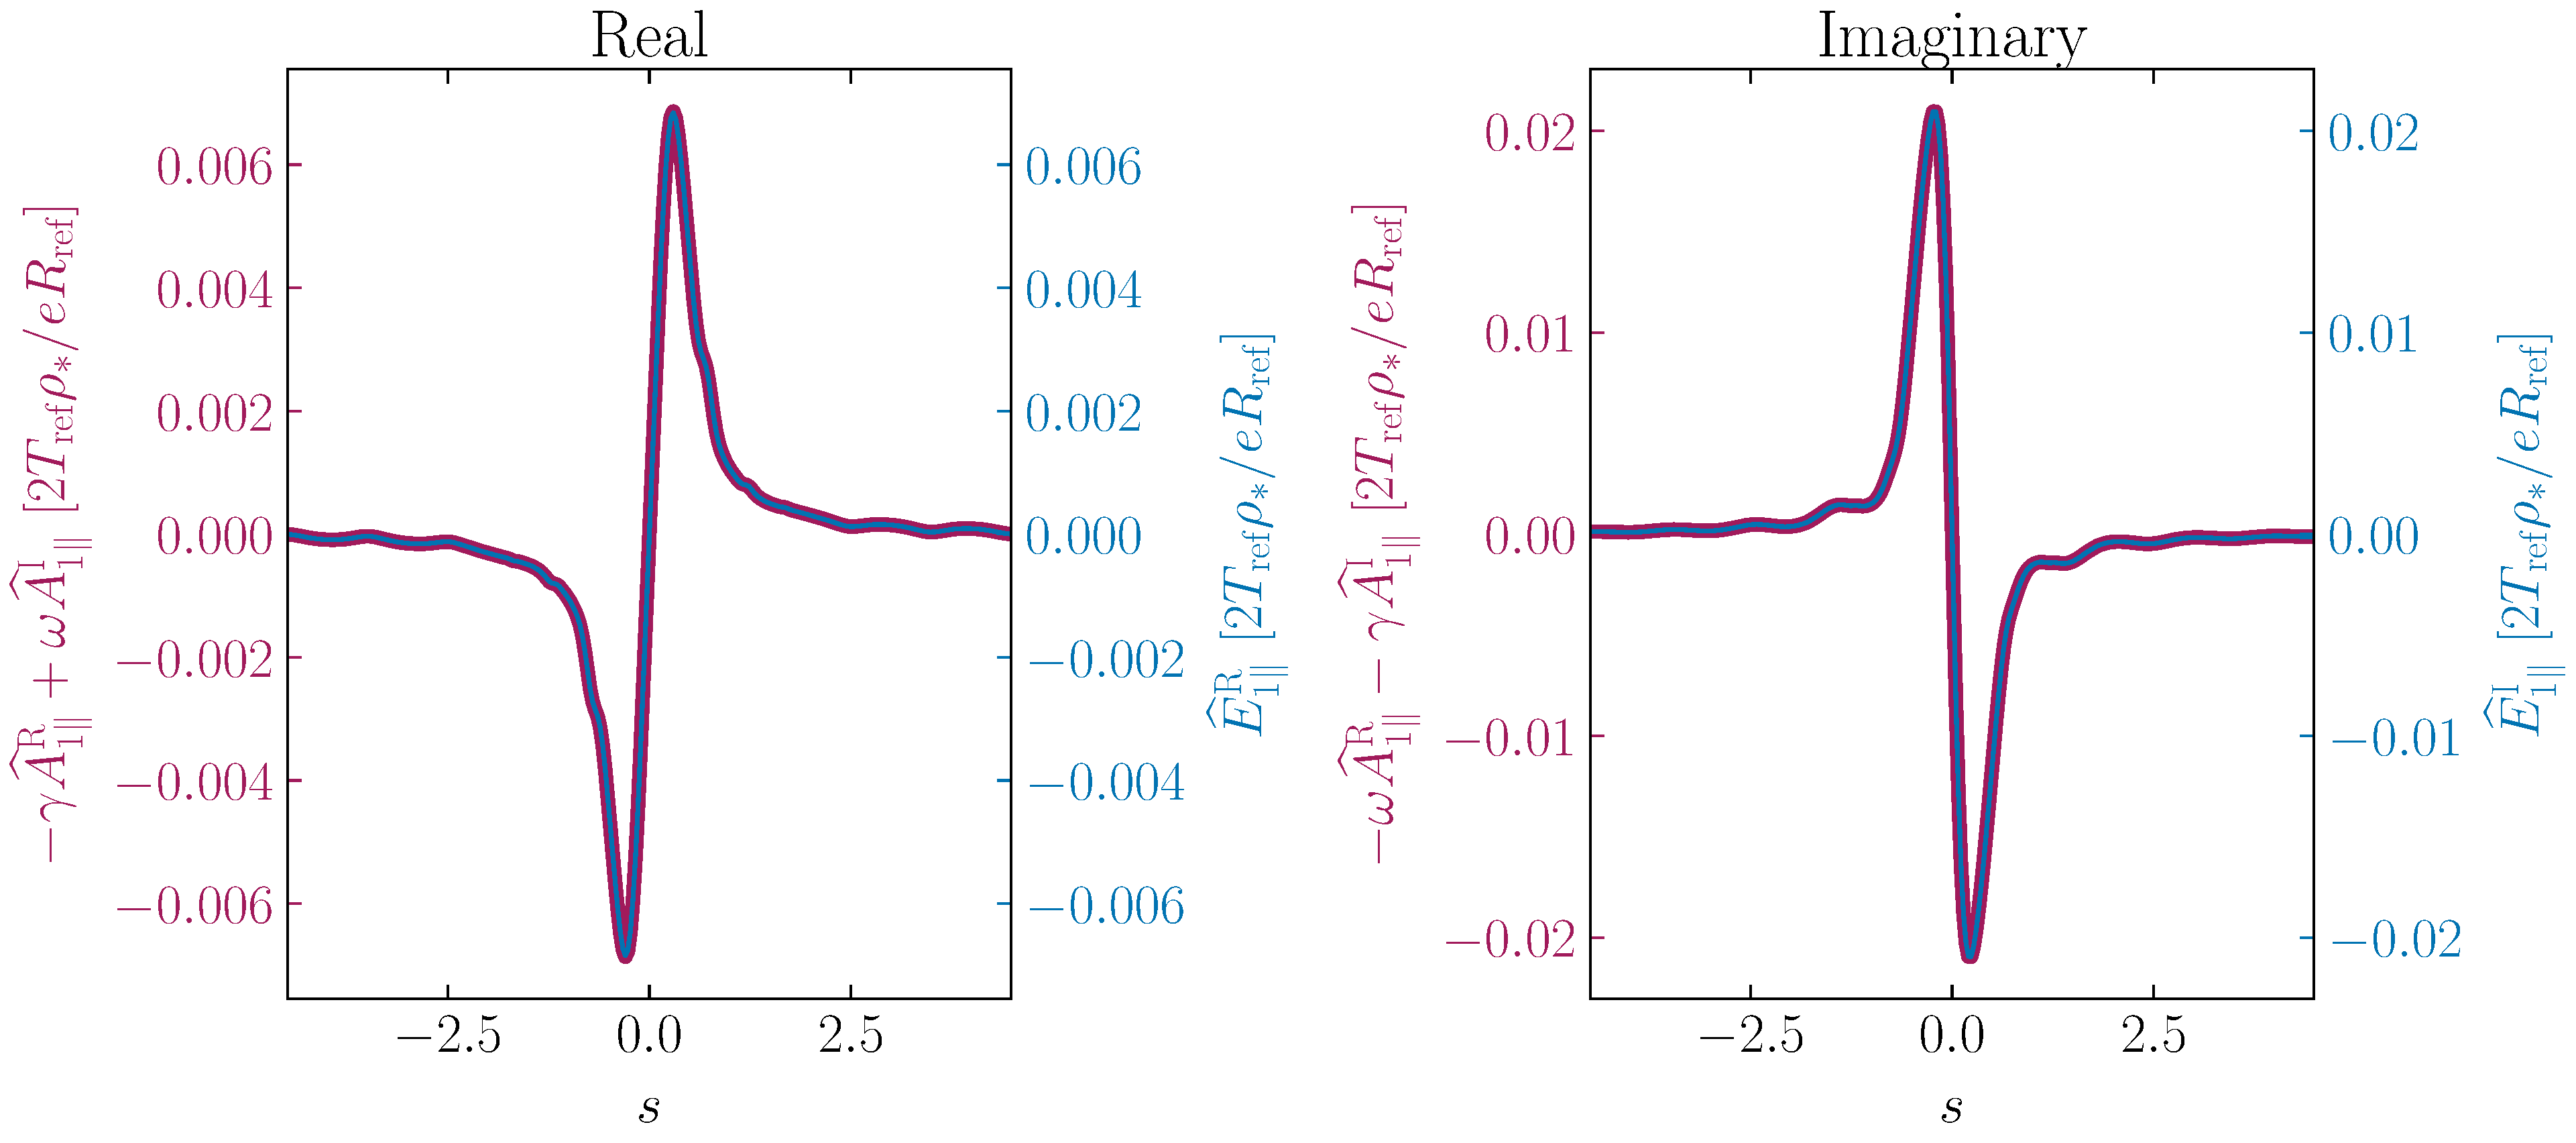
\includegraphics[width=0.9\textwidth]{evaluation/benchmark/f-version/fields/kthrho0.300_beta0.006_fields_f-version.pdf} \\
        $ \beta = 0.8\,\%$ \\
        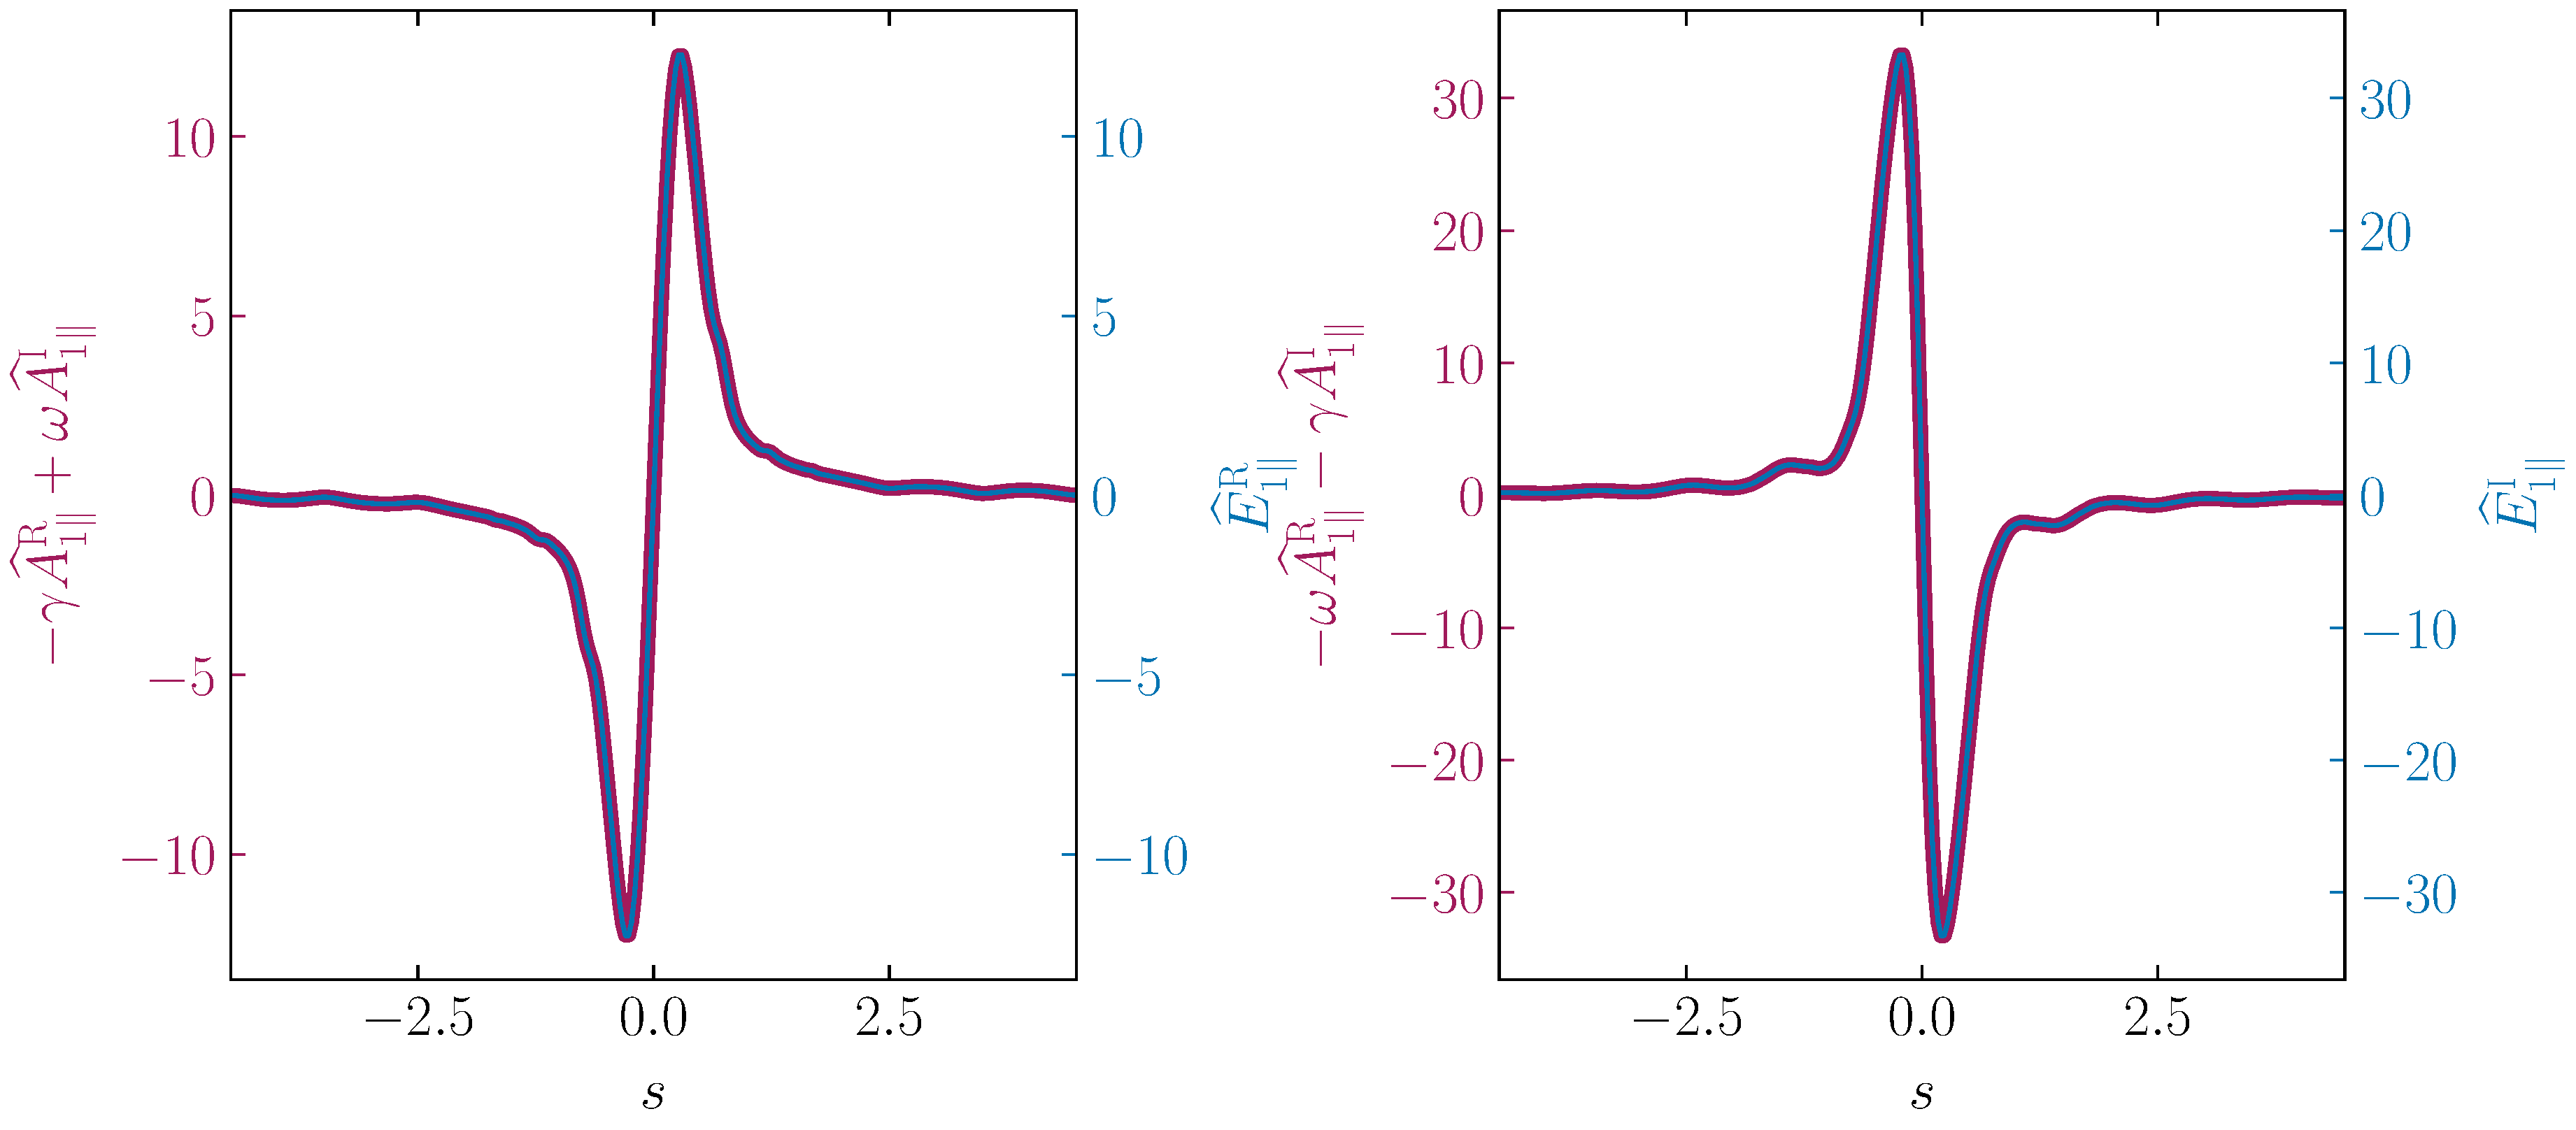
\includegraphics[width=0.9\textwidth]{evaluation/benchmark/f-version/fields/kthrho0.300_beta0.008_fields_f-version.pdf} \\
        $ \beta = 1.0\,\%$ \\
        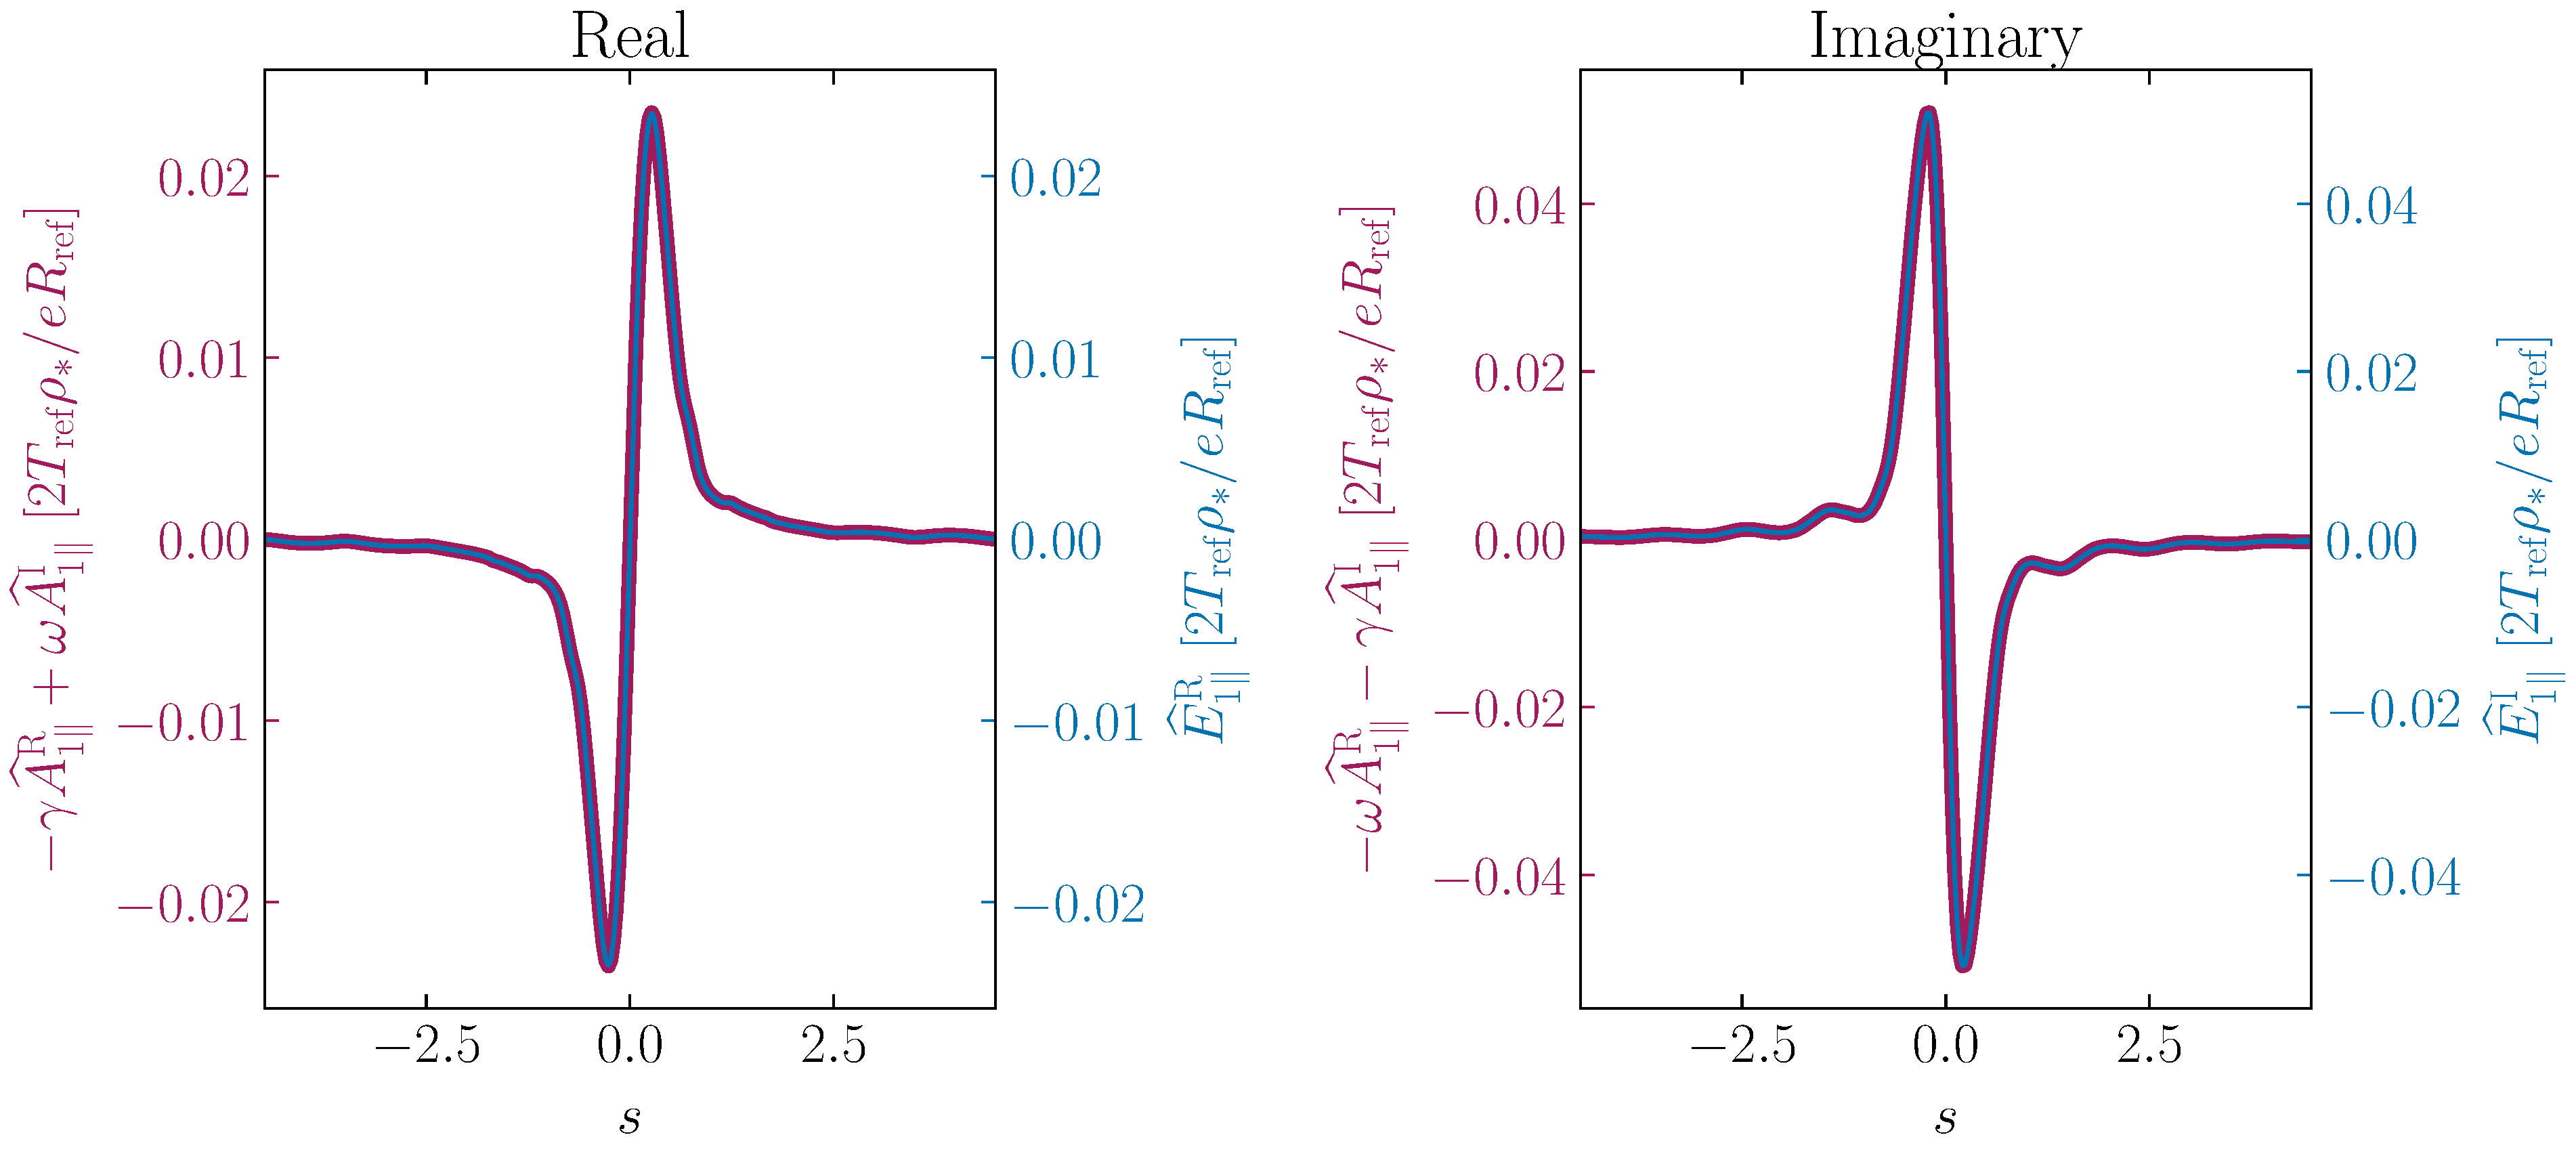
\includegraphics[width=0.9\textwidth]{evaluation/benchmark/f-version/fields/kthrho0.300_beta0.010_fields_f-version.pdf} \\
    \end{tabular}
    % \captionof{figure}{Comparision between real and imaginary part of the induced electric field $\Epar$ and plasma Induction $\Apar$ for various plasma beta $\beta$ for the f-version of {\gkw}}
    % \label{fig:fieldComparisionGVersionAll}
\end{center}

\begin{center}
    % \captionsetup{type=figure}
    \begin{tabular}{c}
        $ \beta = 1.1\,\%$ \\
        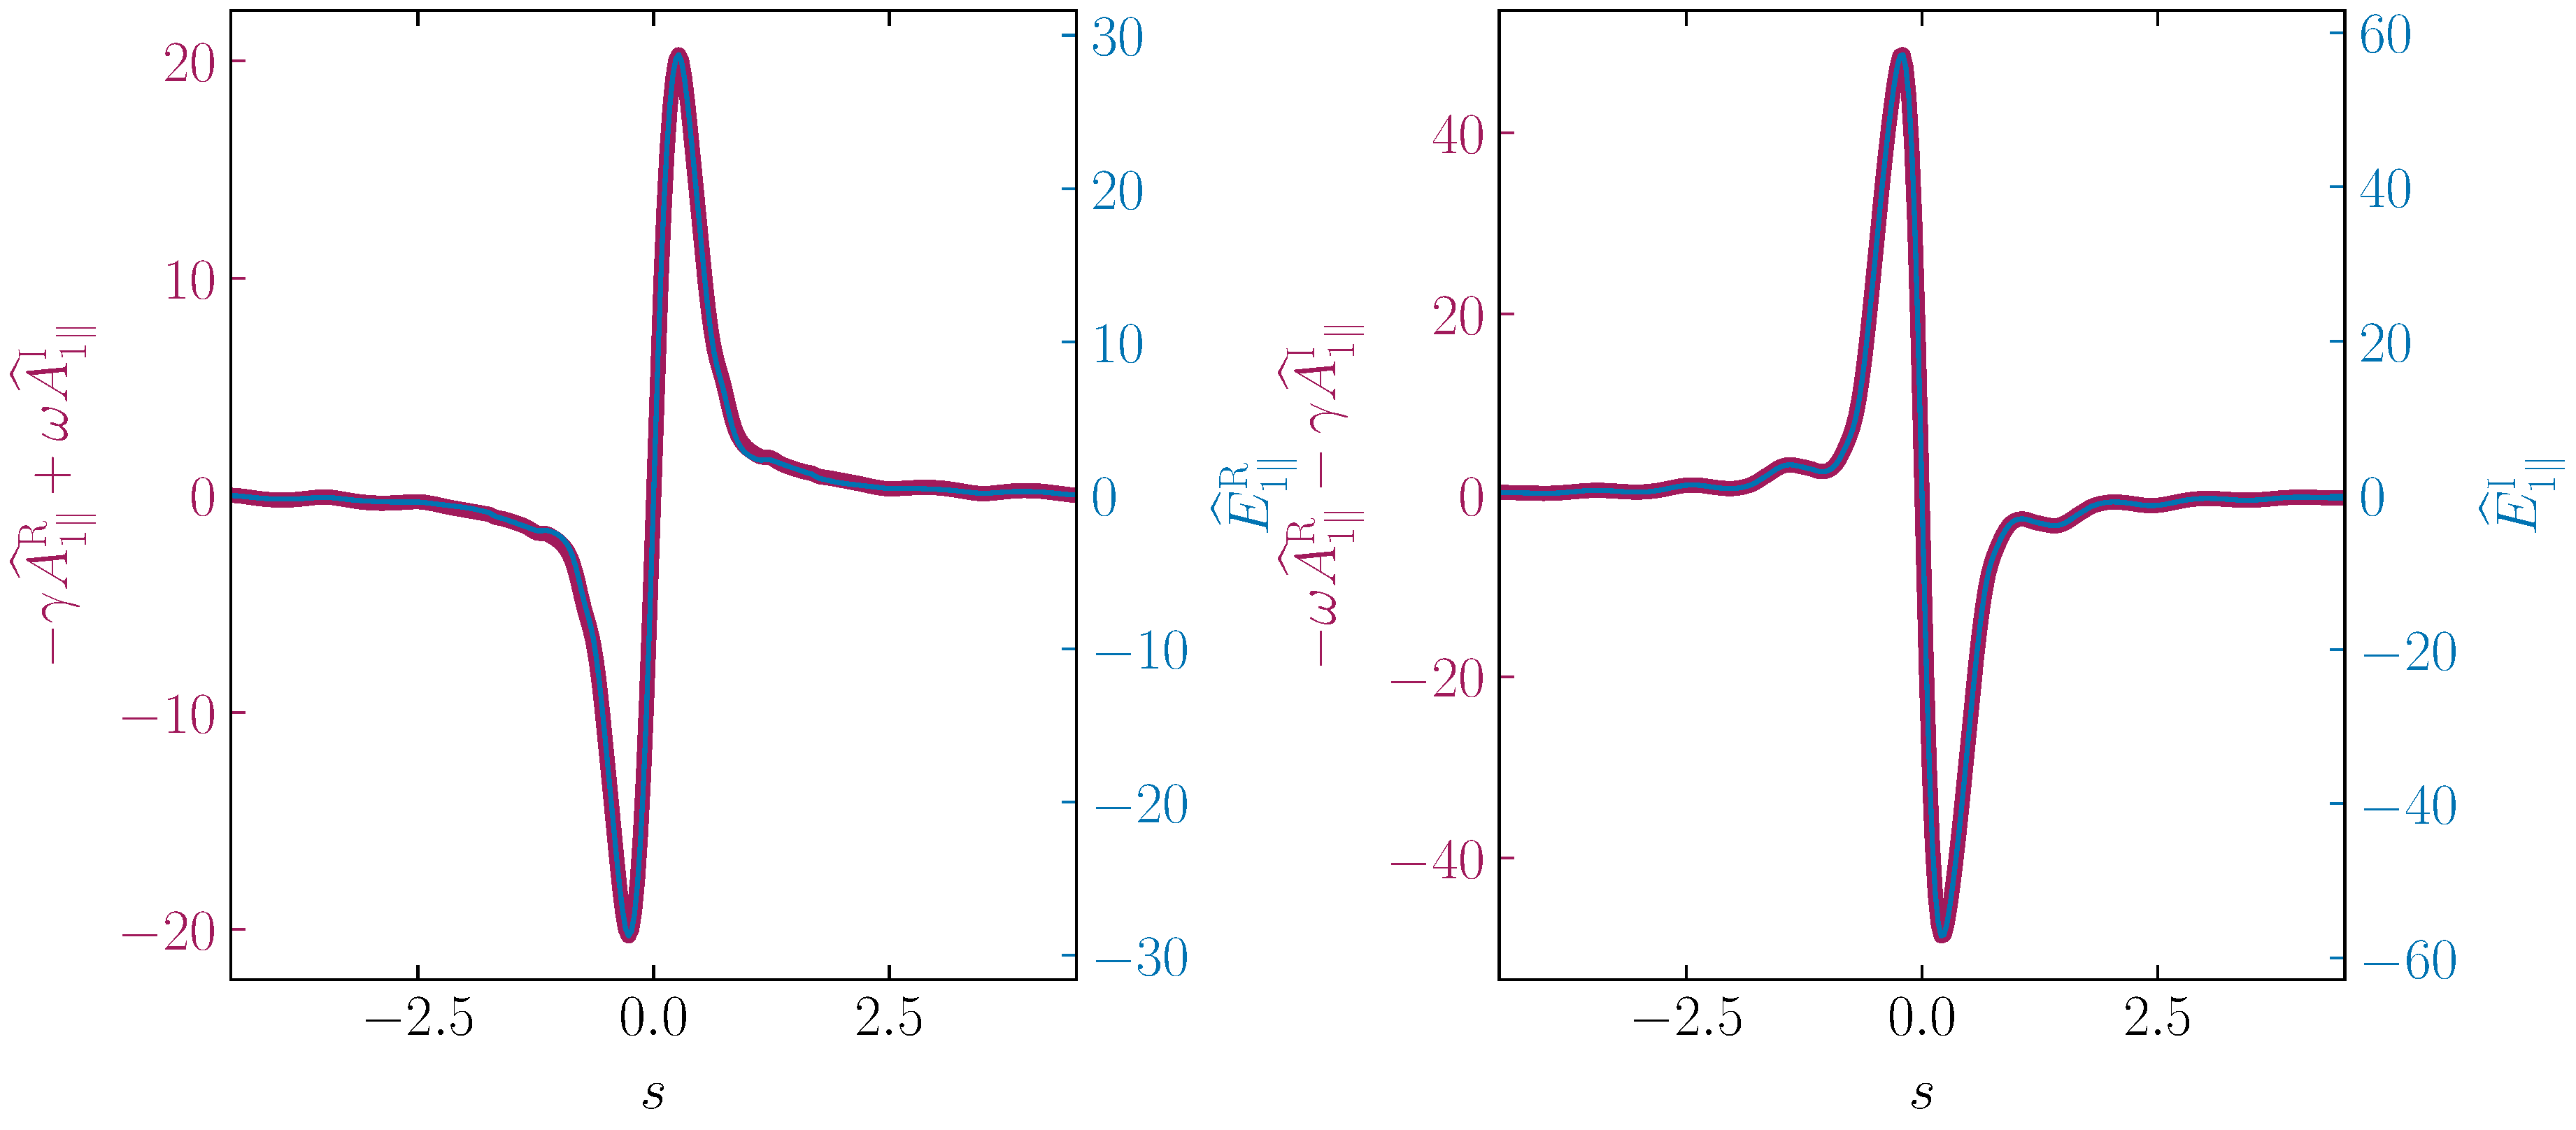
\includegraphics[width=0.9\textwidth]{evaluation/benchmark/f-version/fields/kthrho0.300_beta0.011_fields_f-version.pdf} \\
        $ \beta = 1.2\,\%$ \\
        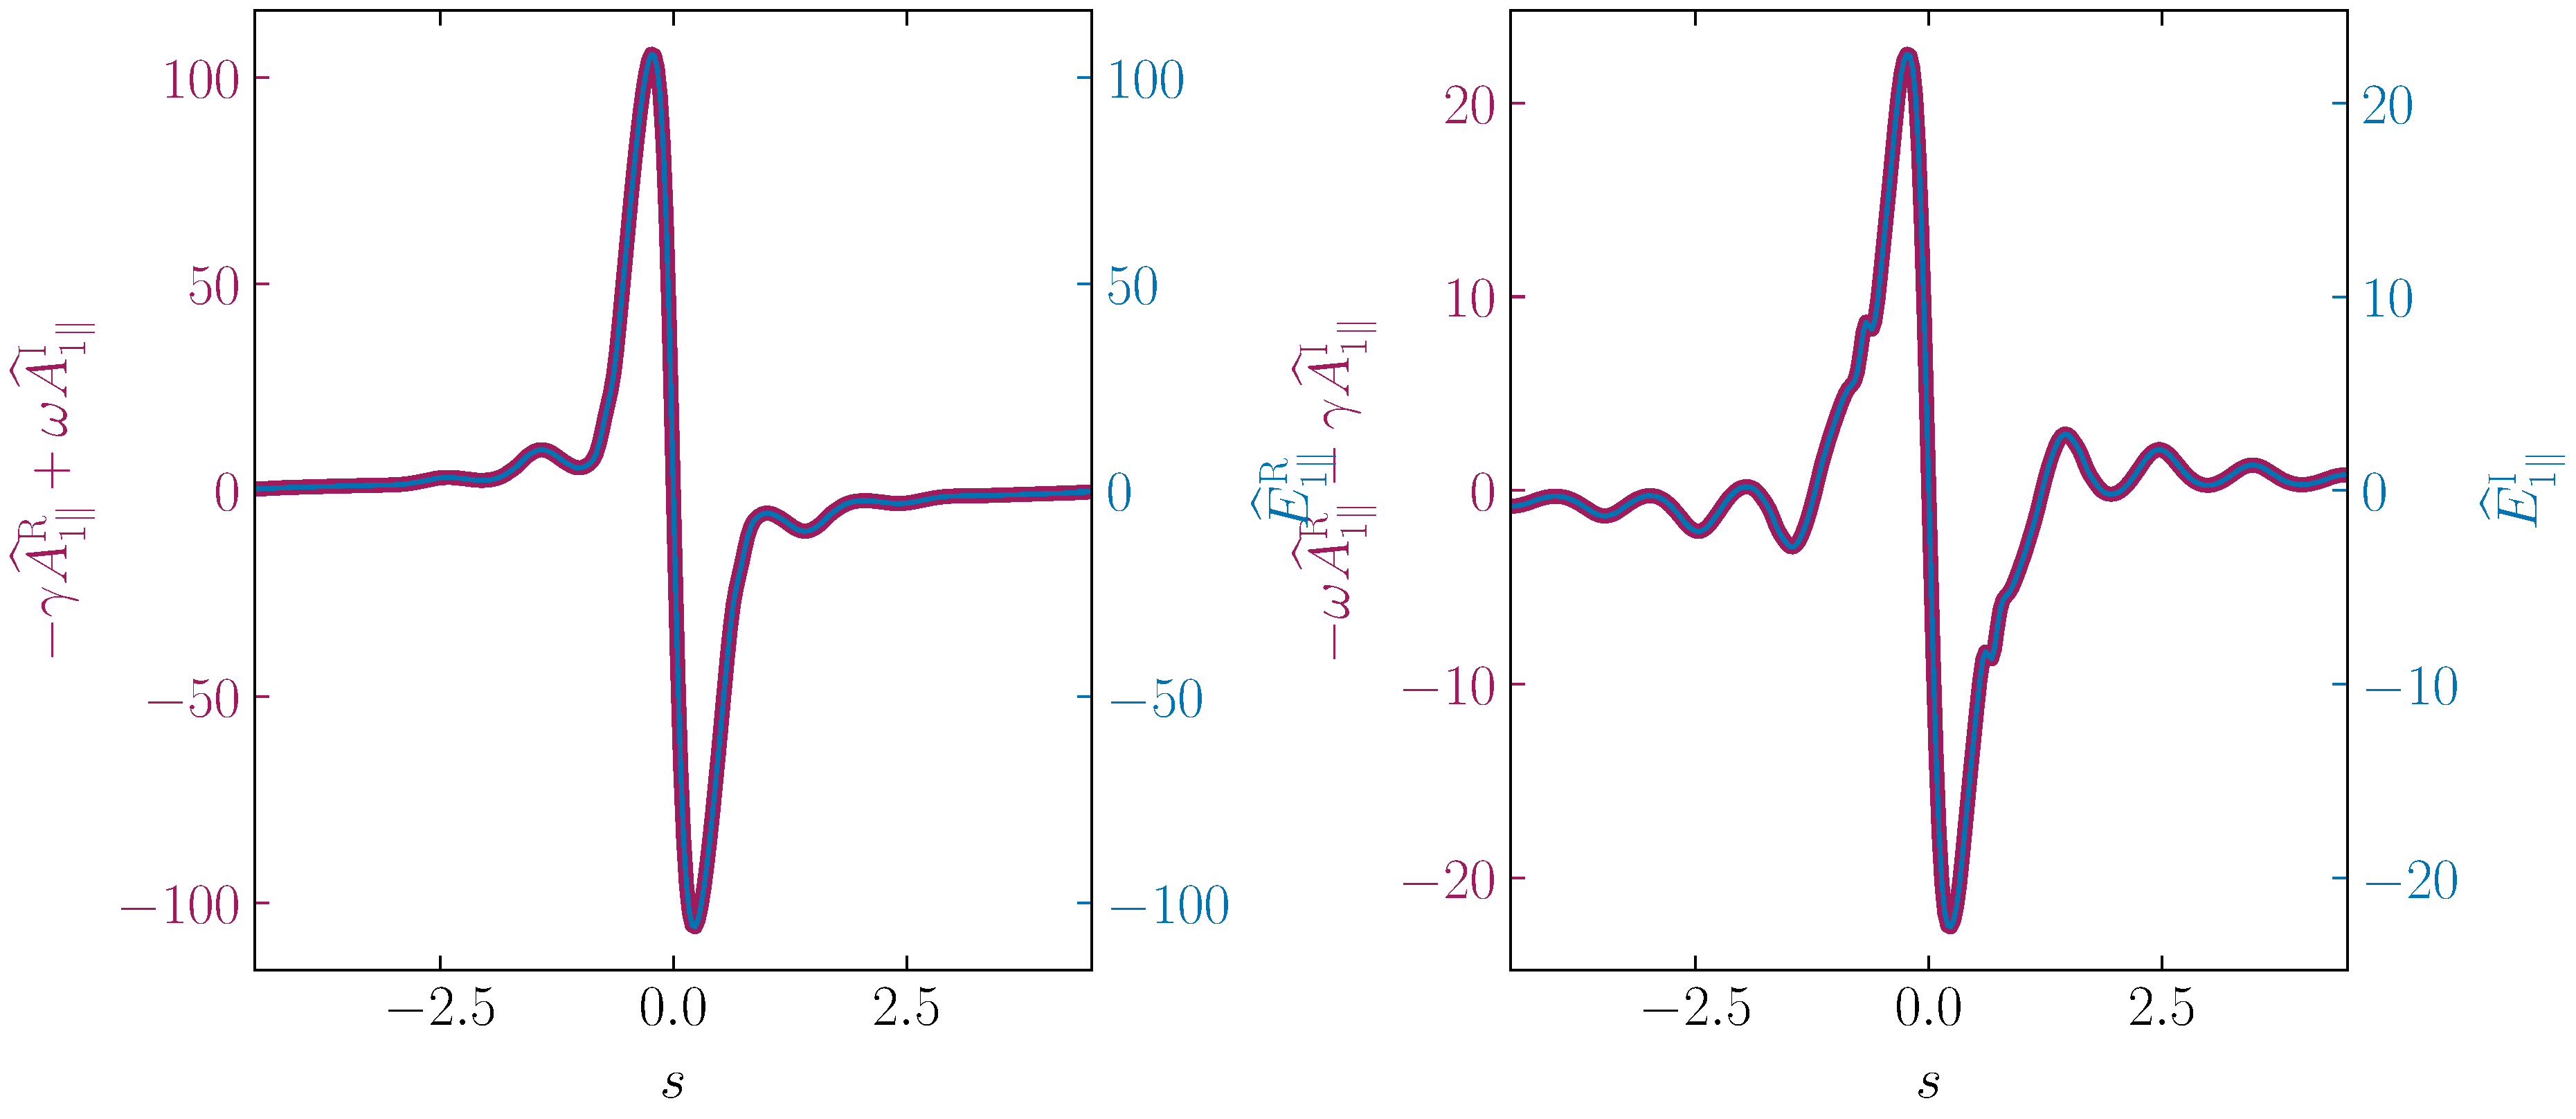
\includegraphics[width=0.9\textwidth]{evaluation/benchmark/f-version/fields/kthrho0.300_beta0.012_fields_f-version.pdf} \\
        $ \beta = 1.4\,\%$ \\
        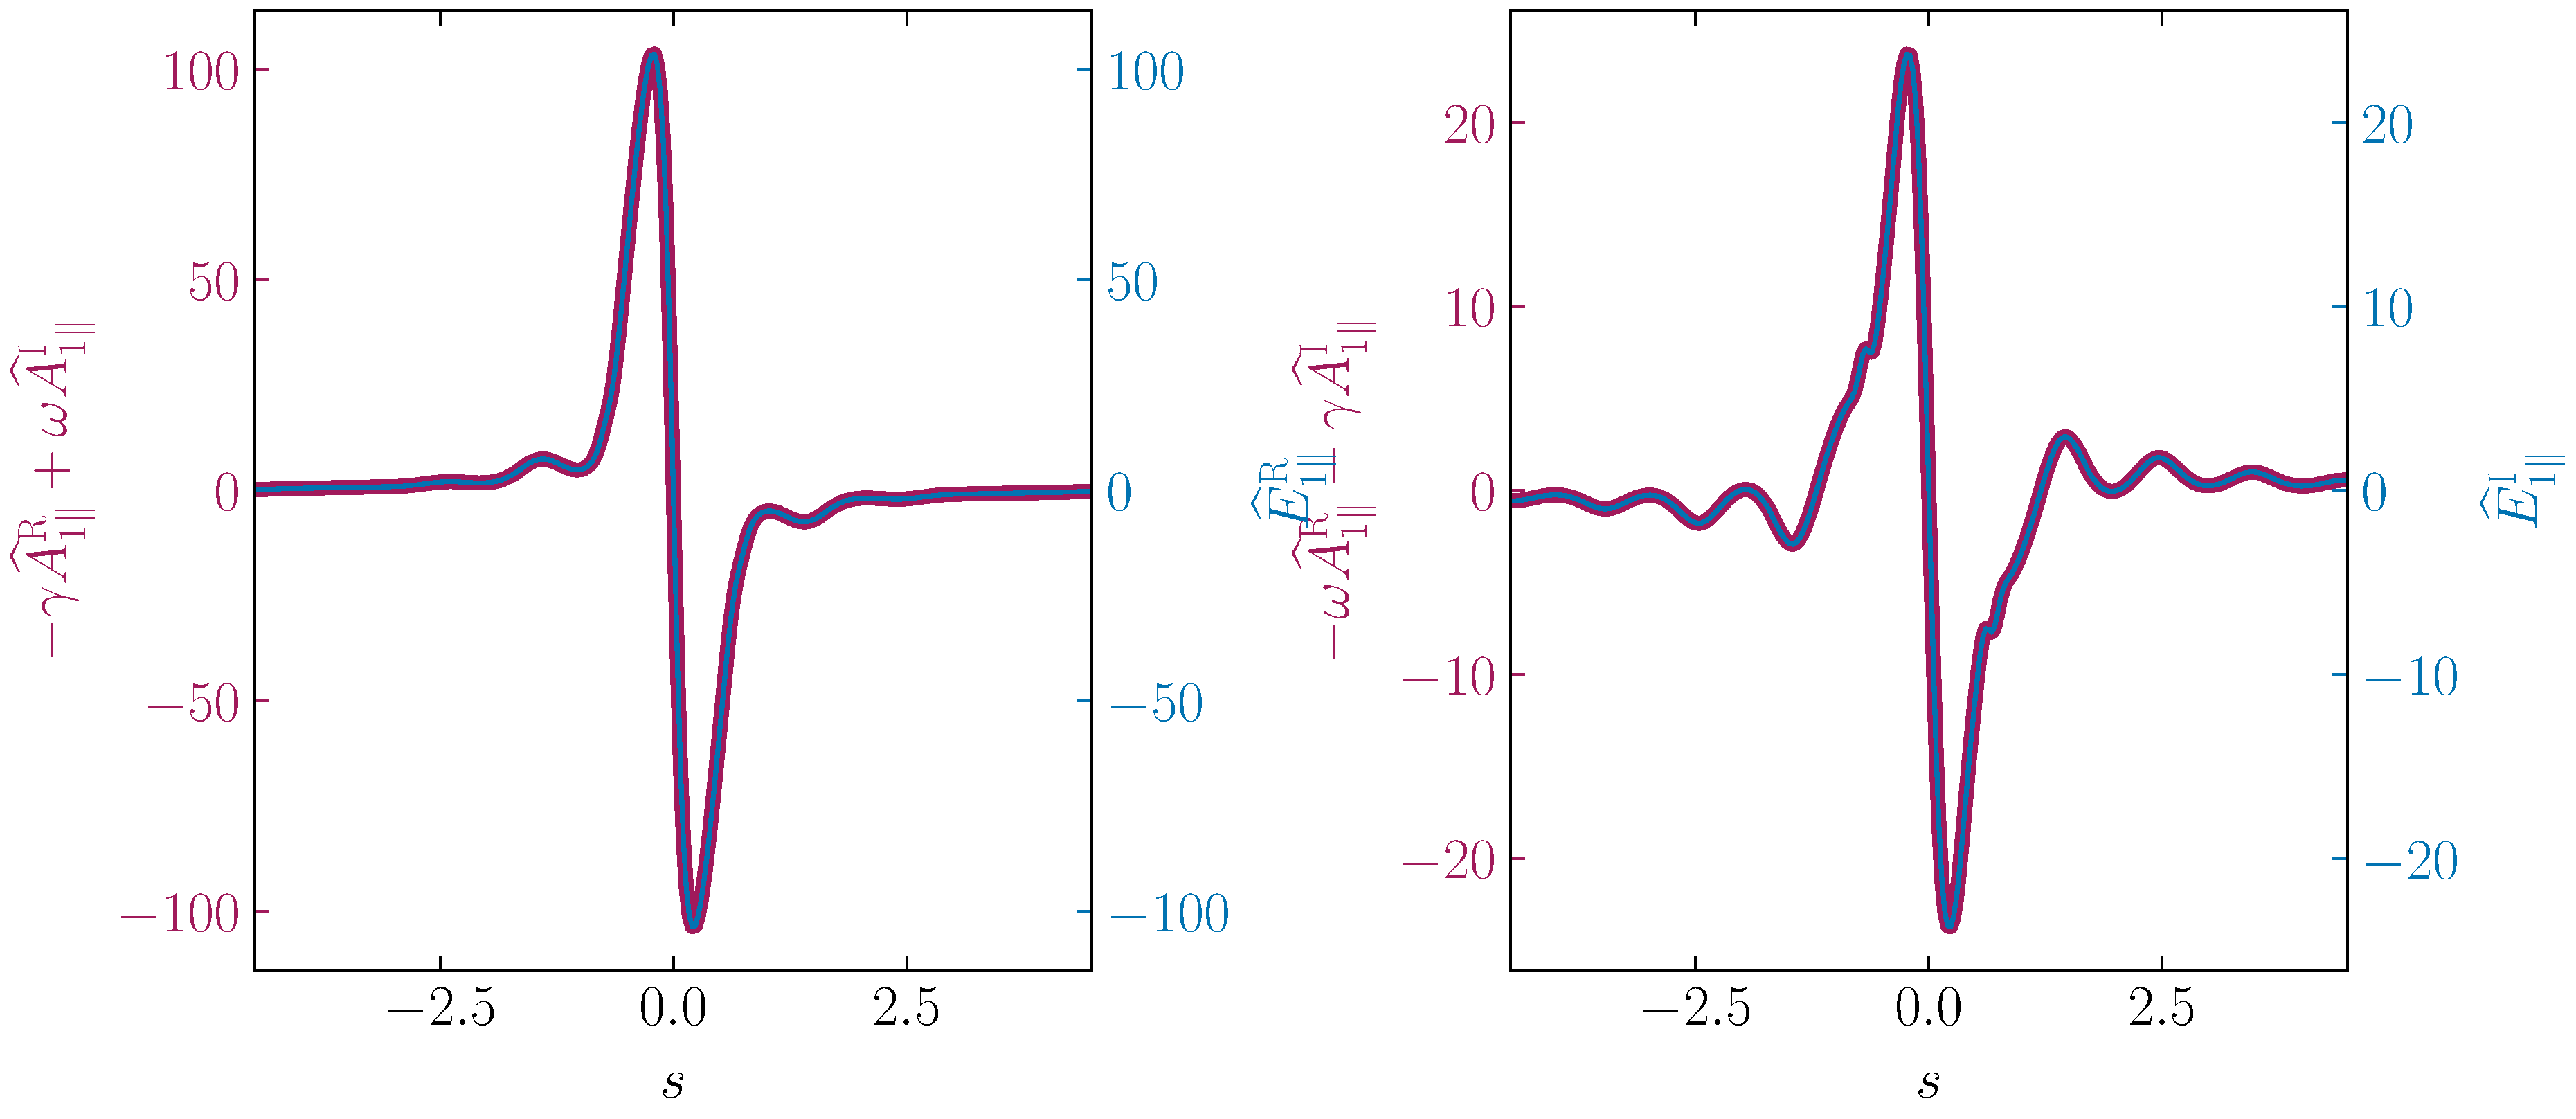
\includegraphics[width=0.9\textwidth]{evaluation/benchmark/f-version/fields/kthrho0.300_beta0.014_fields_f-version.pdf} \\
    \end{tabular}
    % \captionof{figure}{Comparision between real and imaginary part of the induced electric field $\Epar$ and plasma Induction $\Apar$ for various plasma beta $\beta$ for the f-version of {\gkw}}
    % \label{fig:fieldComparisionGVersionAll}
\end{center}

\begin{center}
    % \captionsetup{type=figure}
    \begin{tabular}{c}
        $ \beta = 1.6\,\%$ \\
        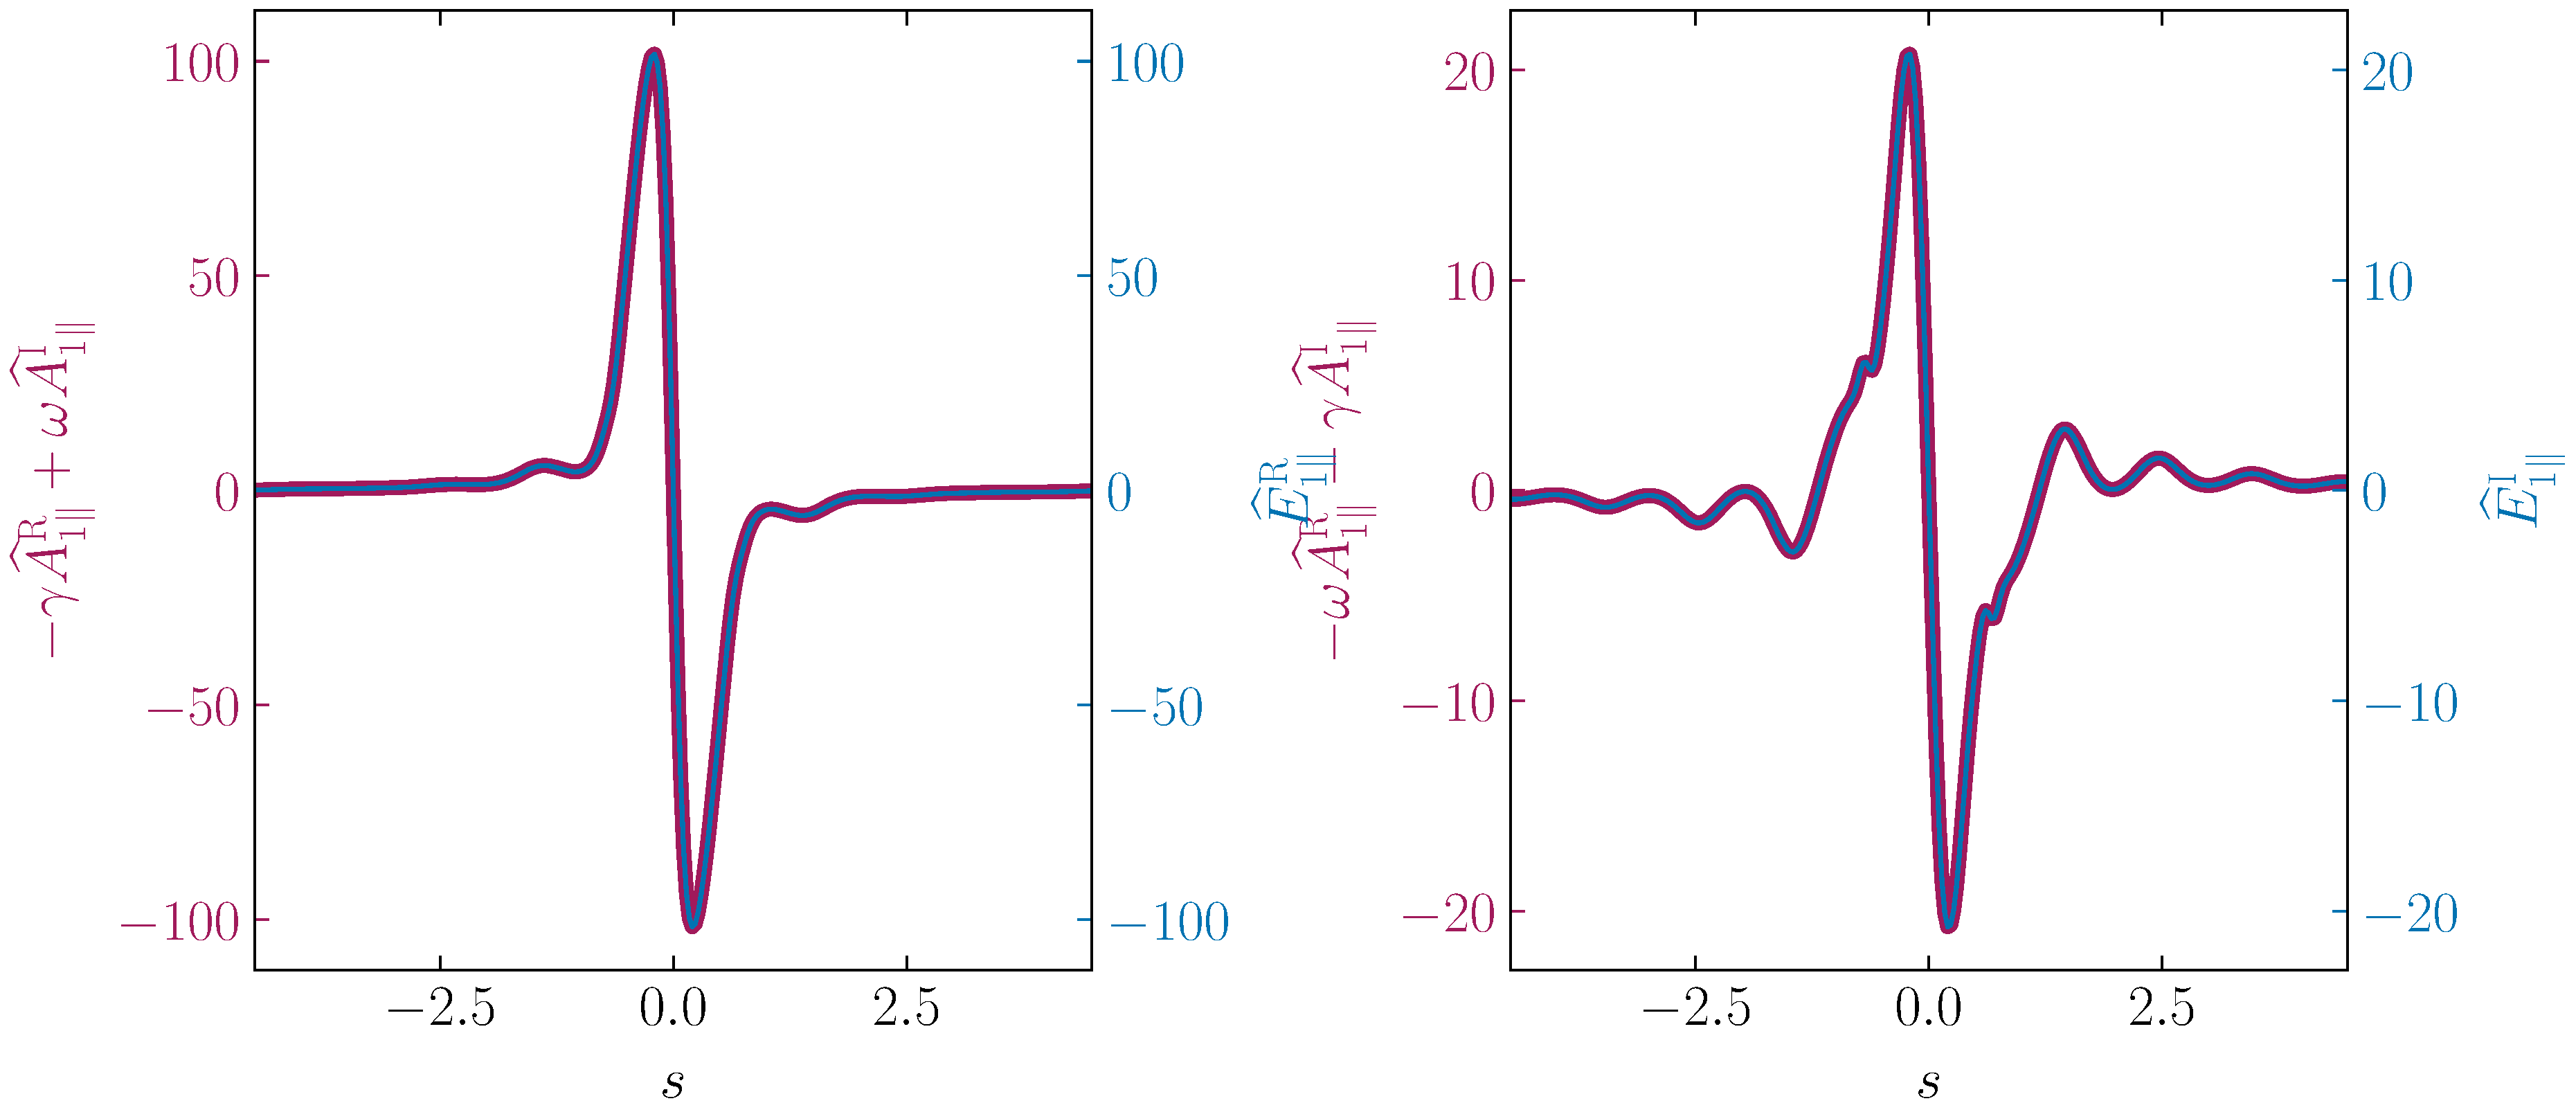
\includegraphics[width=0.9\textwidth]{evaluation/benchmark/f-version/fields/kthrho0.300_beta0.016_fields_f-version.pdf} \\
        $ \beta = 1.8\,\%$ \\
        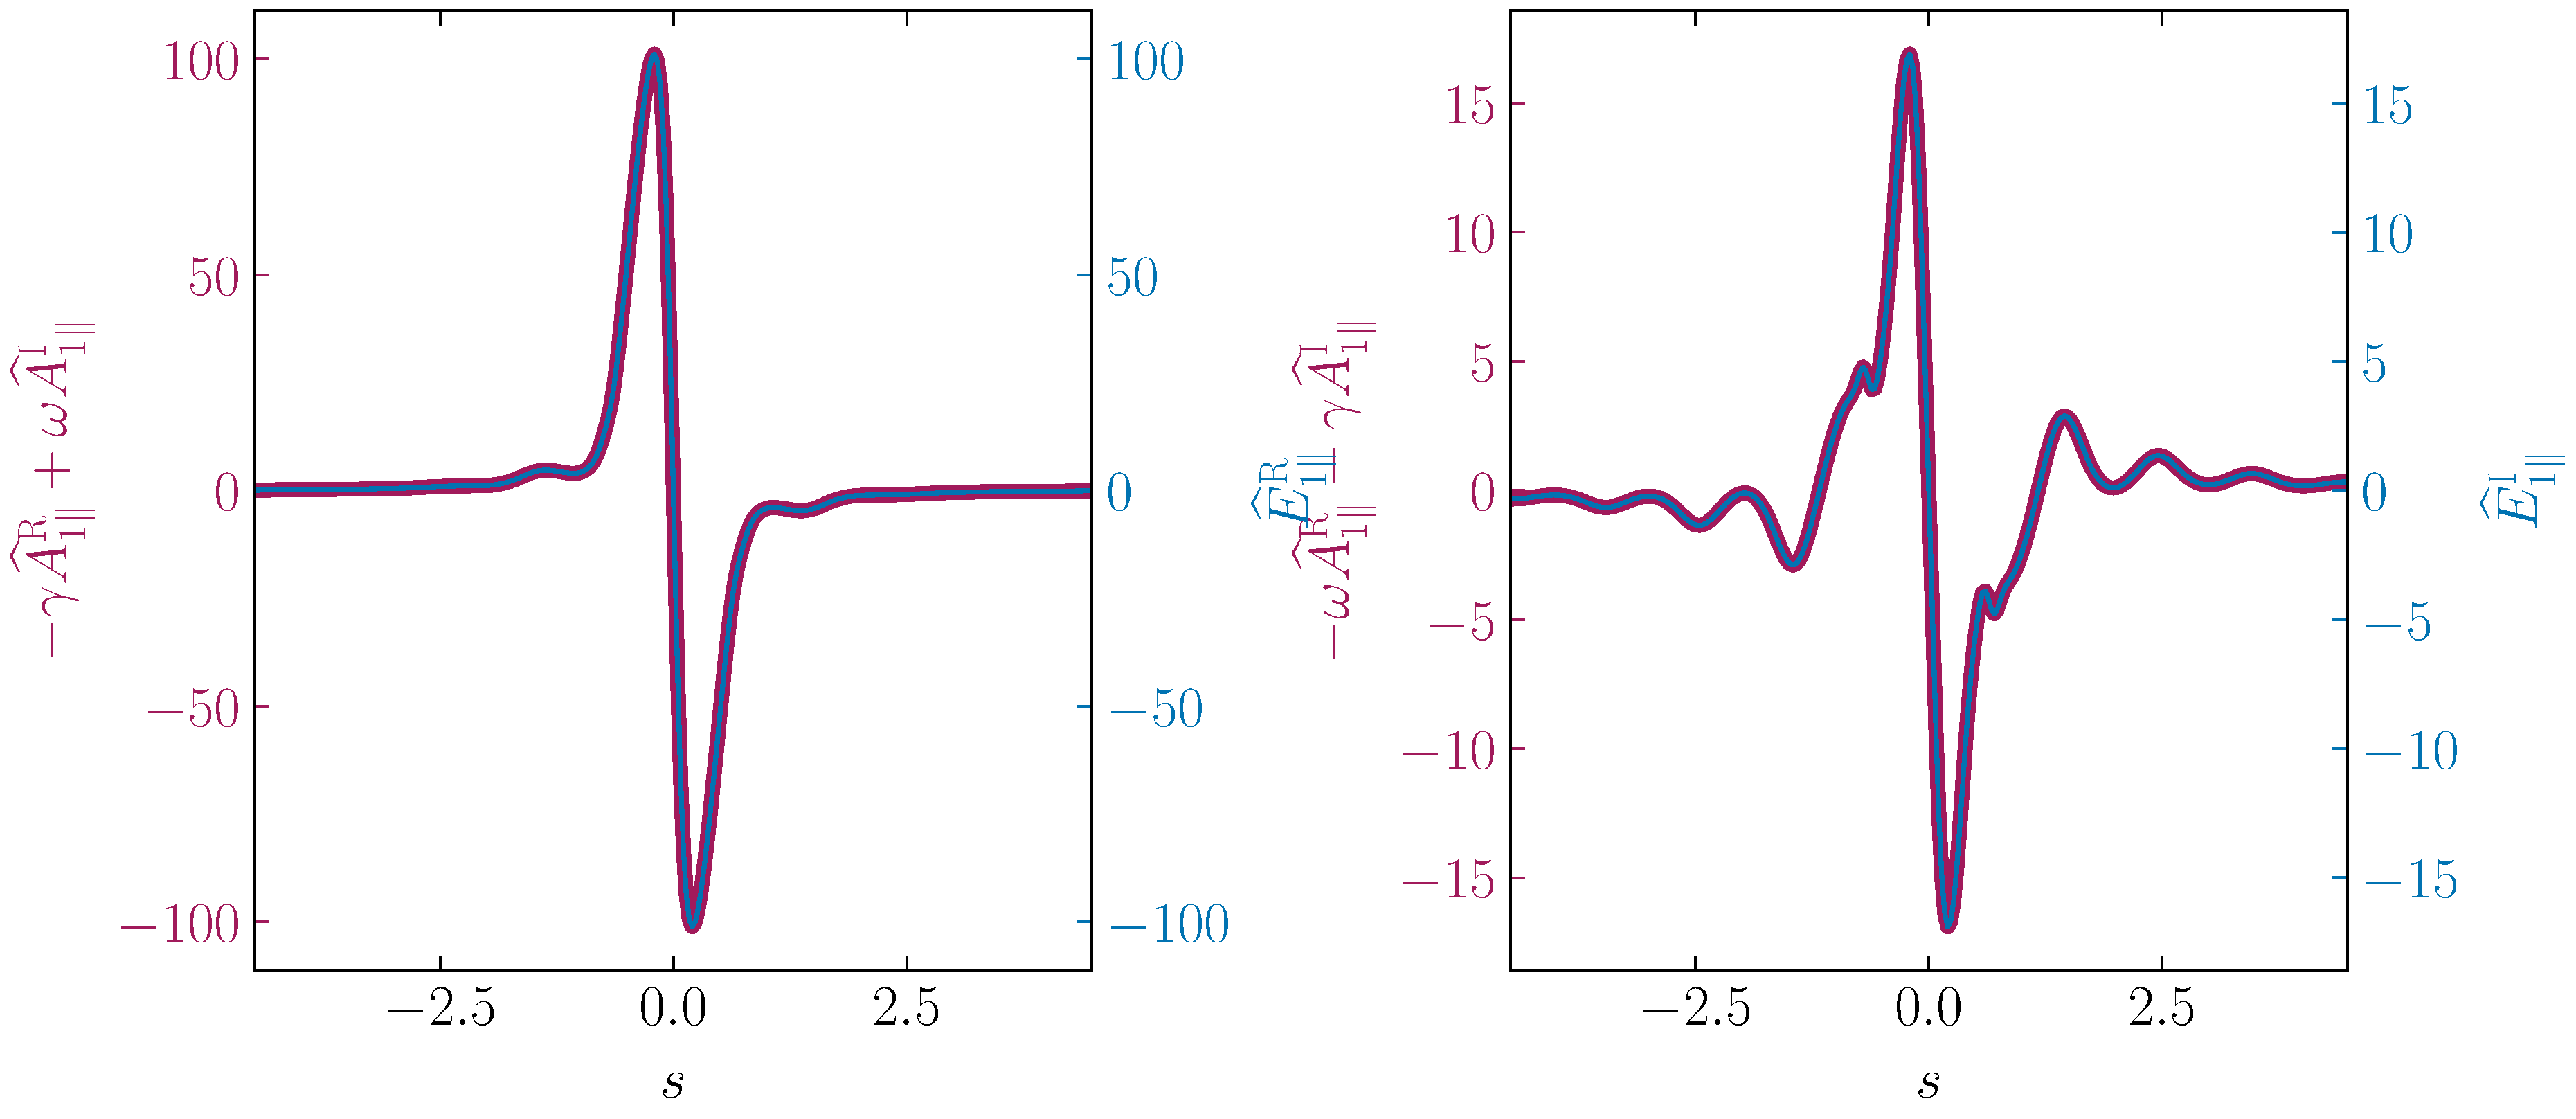
\includegraphics[width=0.9\textwidth]{evaluation/benchmark/f-version/fields/kthrho0.300_beta0.018_fields_f-version.pdf} \\
        $ \beta = 2.0\,\%$ \\
        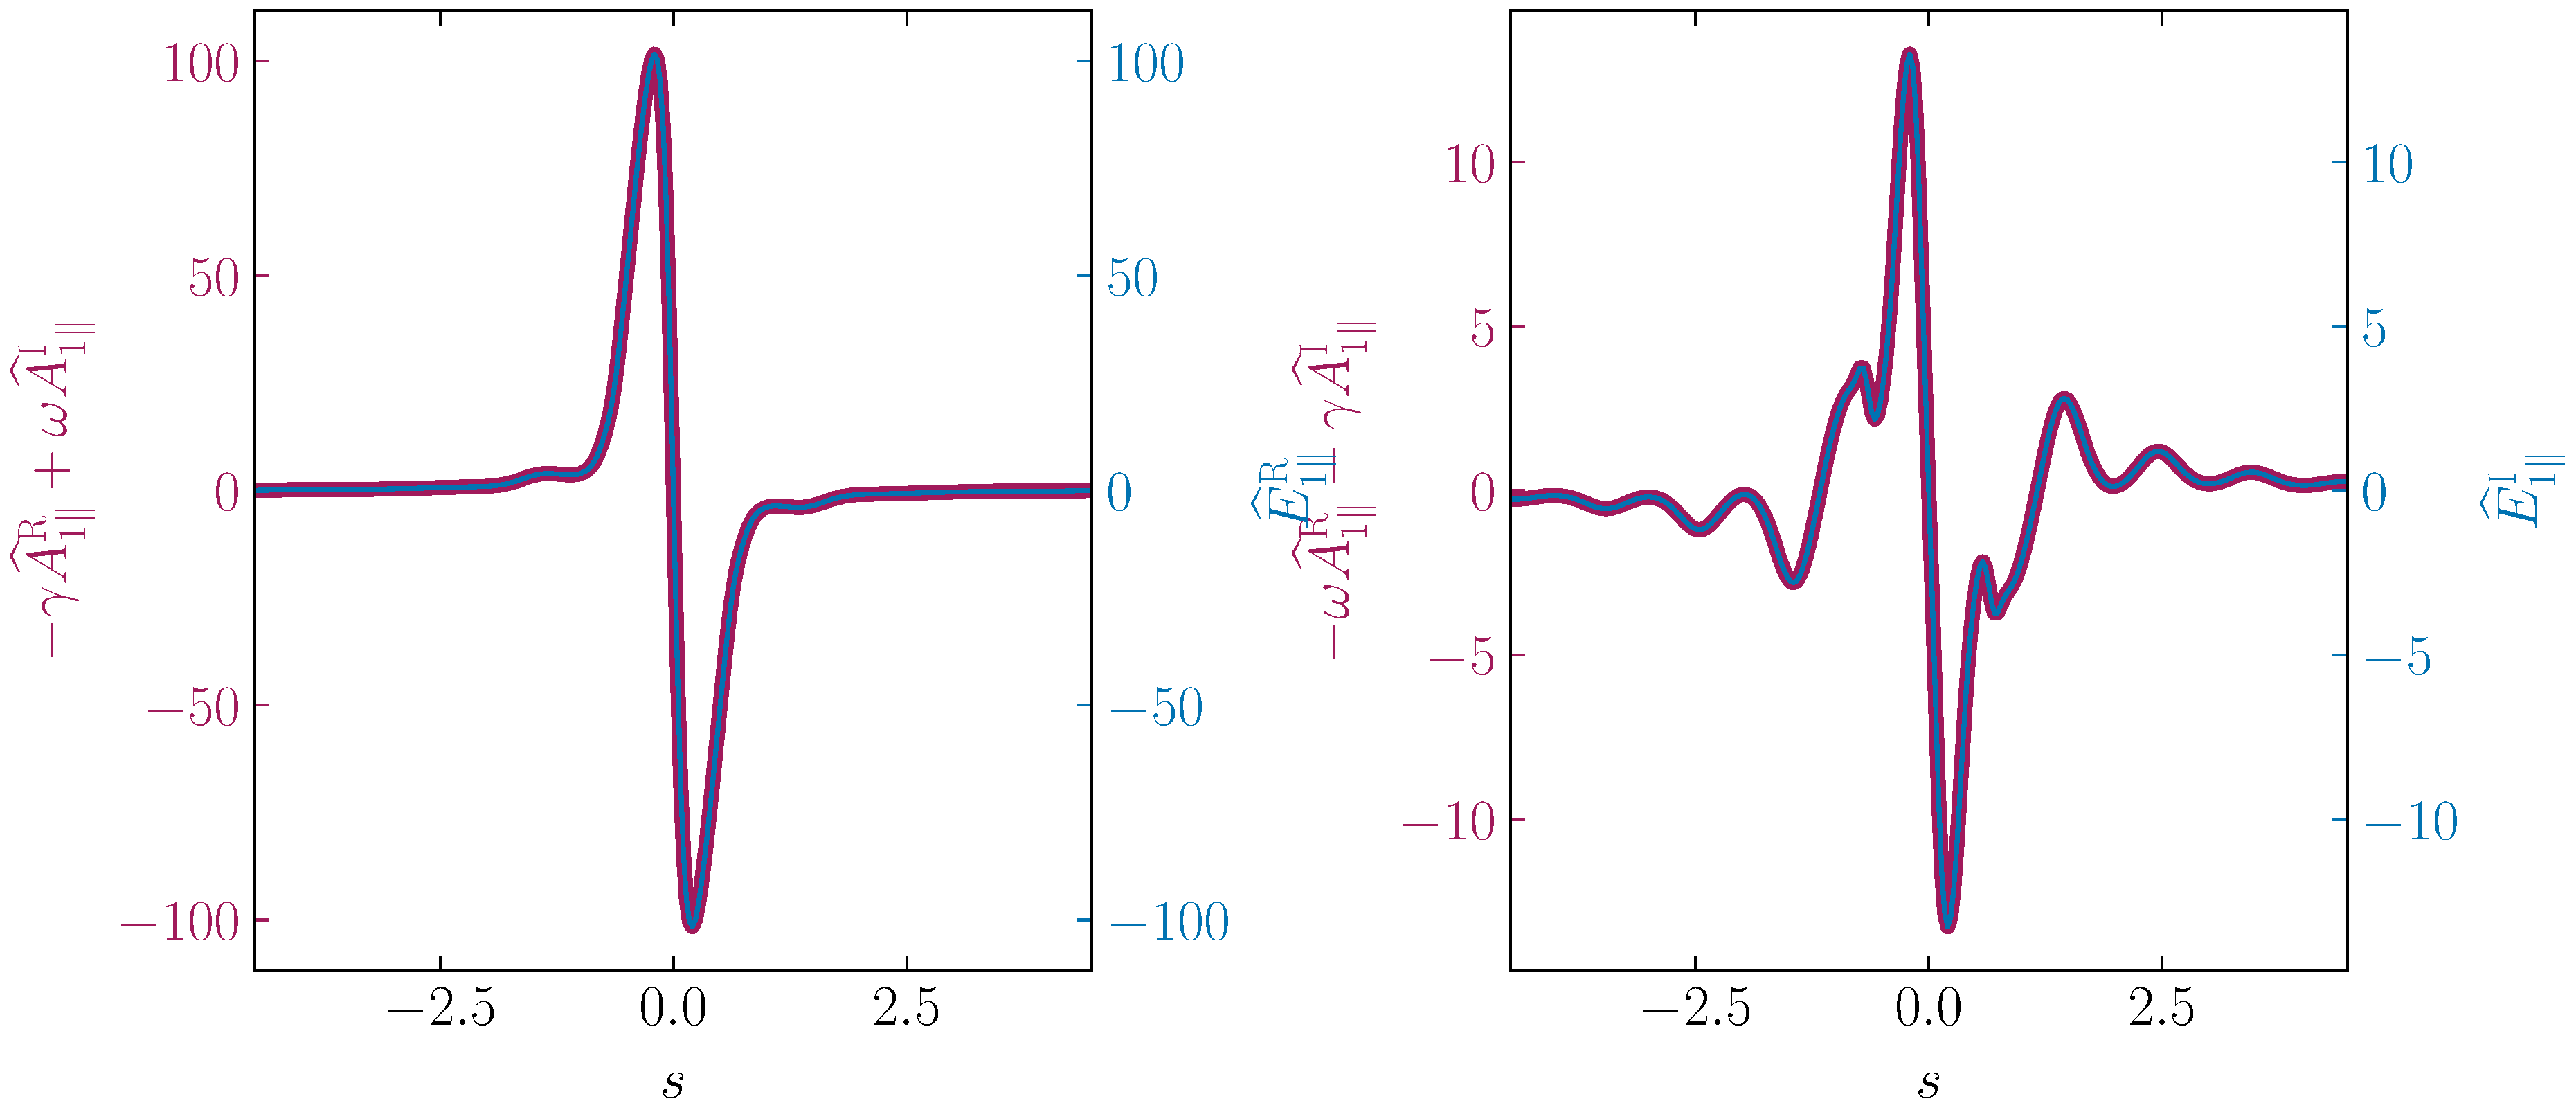
\includegraphics[width=0.9\textwidth]{evaluation/benchmark/f-version/fields/kthrho0.300_beta0.020_fields_f-version.pdf} \\
    \end{tabular}
    % \captionof{figure}{Comparision between real and imaginary part of the induced electric field $\Epar$ and plasma Induction $\Apar$ for various plasma beta $\beta$ for the f-version of {\gkw}}
    % \label{fig:fieldComparisionGVersionAll}
\end{center}

\begin{center}
    % \captionsetup{type=figure}
    \begin{tabular}{c}
        $ \beta = 2.2\,\%$ \\
        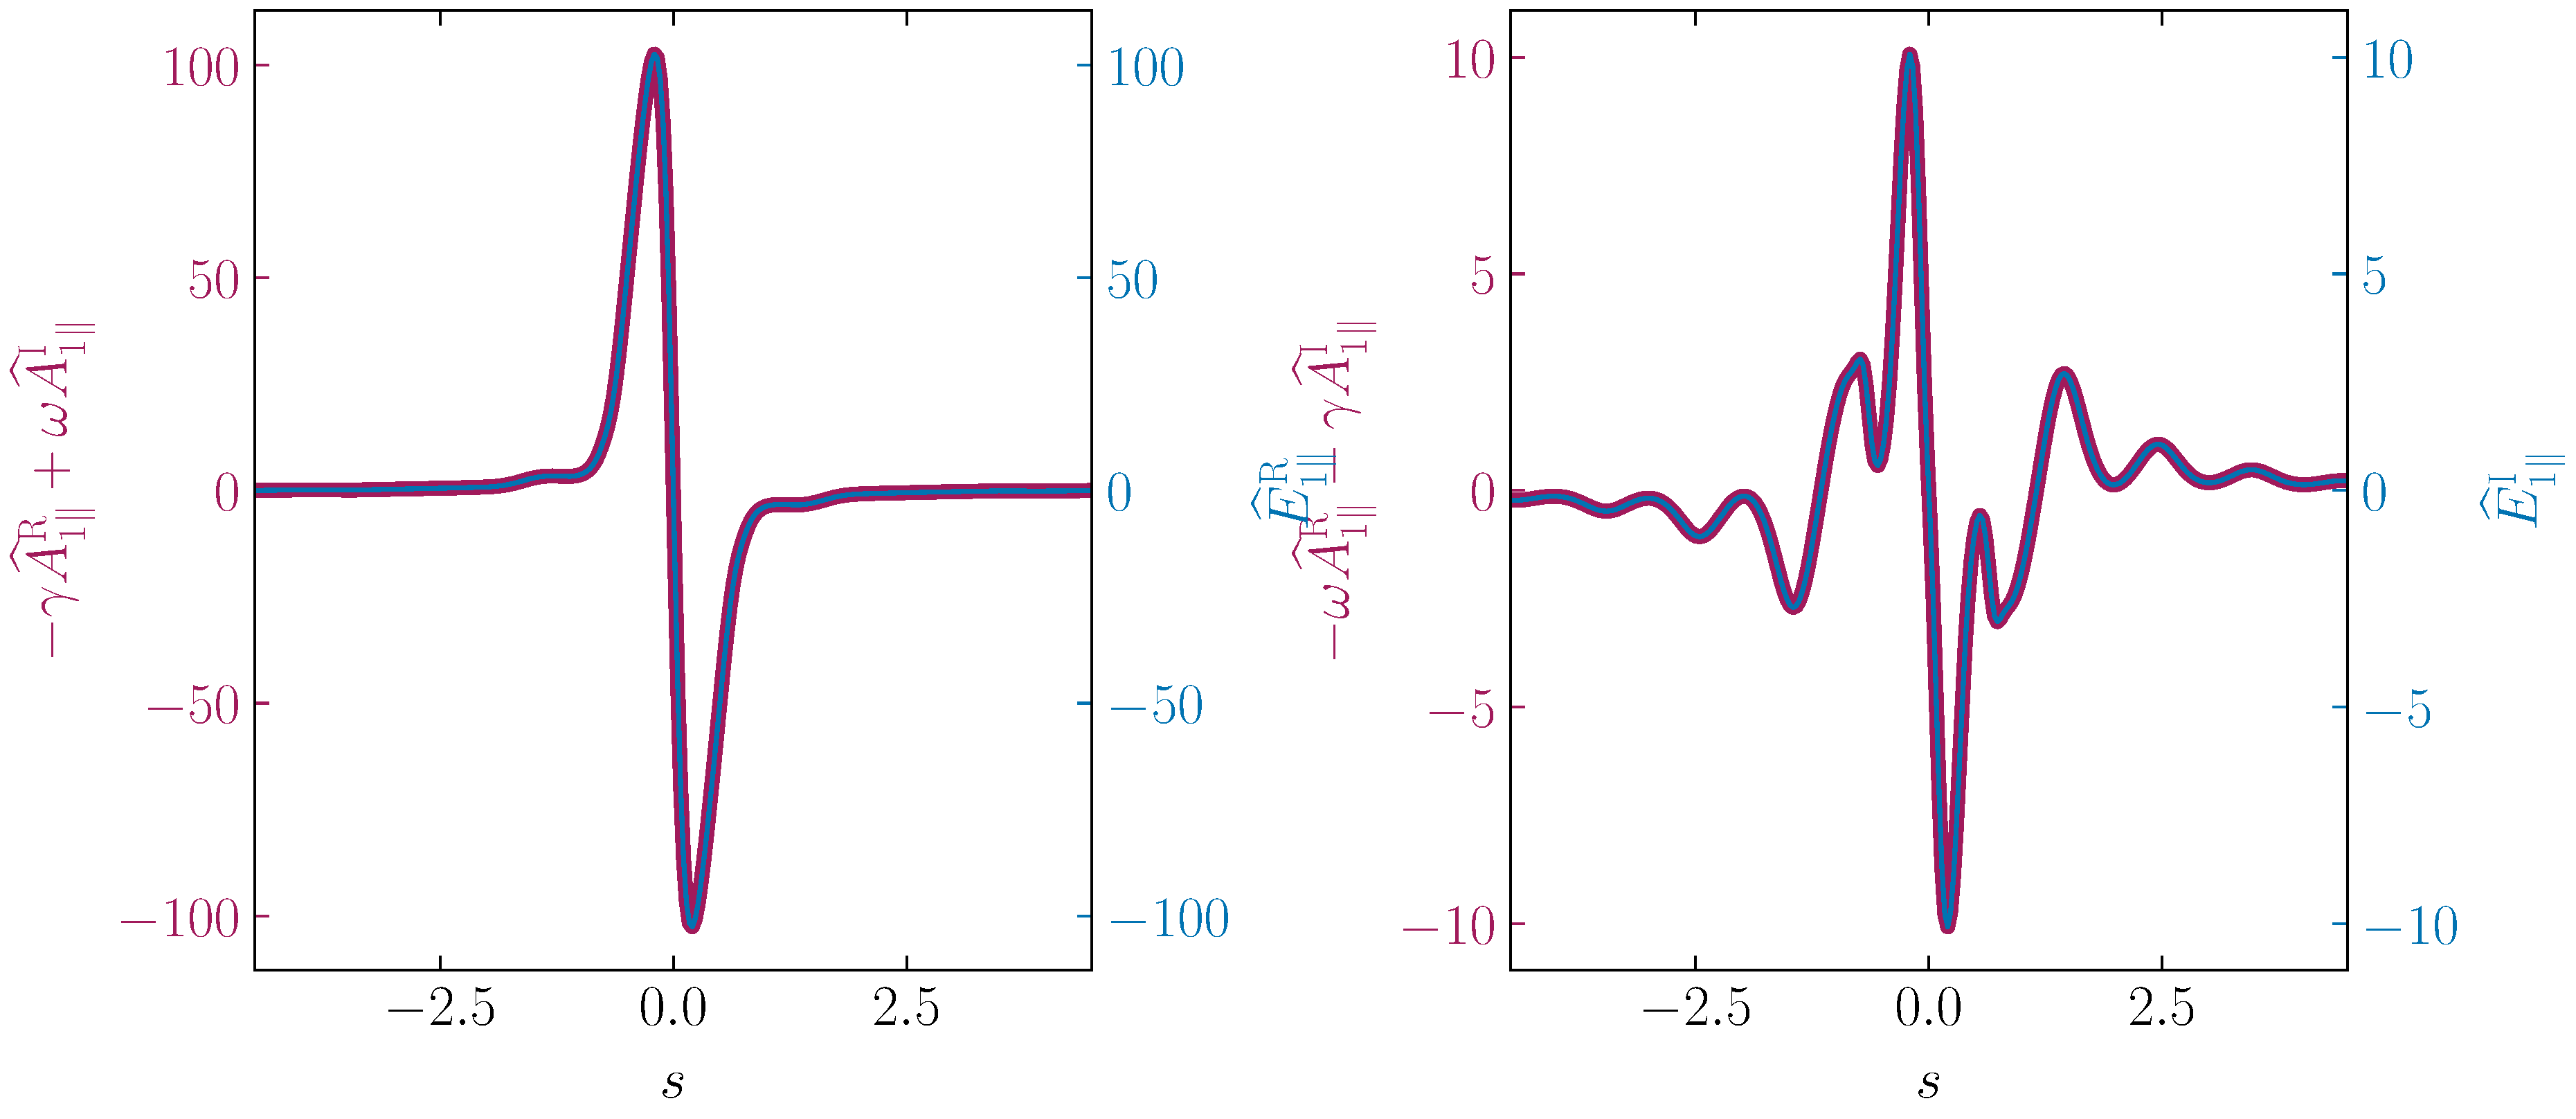
\includegraphics[width=0.9\textwidth]{evaluation/benchmark/f-version/fields/kthrho0.300_beta0.022_fields_f-version.pdf} \\
    \end{tabular}
    % \captionof{figure}{Comparision between real and imaginary part of the induced electric field $\Epar$ and plasma Induction $\Apar$ for various plasma beta $\beta$ for the f-version of {\gkw}}
    % \label{fig:fieldComparisionGVersionAll}
\end{center}
    %
    % Literatur
    %\nocite{*}
    \NewPage
    \bibliographystyle{literaturestyle.bst}
    \bibliography{literature.bib}
    %
    % Eid
    \newpage
\chapter*{Eidesstattliche Erklärung}
\label{sec:eid}
\thispagestyle{empty}

\addcontentsline{toc}{chapter}{Eidesstattliche Erklärung}
\vspace*{0.1cm}
Hiermit erkläre ich, Manuel Lippert, dass ich die vorliegende Arbeit selbständig und ohne Benutzung anderer als der angegebenen Hilfsmittel angefertigt habe.
\bigskip
Alle Stellen, die wörtlich oder sinngemäß aus veröffentlichten oder nicht veröffentlichten Schriften entnommen wurden, sind als solche kenntlich gemacht.
\bigskip
Die Arbeit hat in gleicher oder ähnlicher Form noch keiner anderen Prüfungsbehörde vorgelegen.
\vspace{3cm}

\noindent Bayreuth, den 02.10.2024
\begin{flushright}
$\overline{~~~~~~~~~~\mbox{Manuel Lippert}~~~~~~~~~~}$
\end{flushright}
\end{document}